\documentclass[sigconf,anonymous]{aamas}
\usepackage{balance}
\usepackage{booktabs}
\usepackage{multirow}
\usepackage{xcolor}
% Generated by paperengine.provenance -- do not edit by hand.
% Every number printed in this paper is defined here and traced to a run record.

% a bold not extremal pct: aamas_make_all
\newcommand{\nABoldNotExtremalPct}{18.1\%}
% a bold single groups: aamas_make_all
\newcommand{\nABoldSingleGroups}{2656}
% a bold tied: aamas_make_all
\newcommand{\nABoldTied}{65}
% a bold topk: aamas_make_all
\newcommand{\nABoldTopk}{0}
% a comparisons: aamas_make_all
\newcommand{\nAComparisons}{2109}
% a comparisons per table: aamas_make_all
\newcommand{\nAComparisonsPerTable}{9}
% a comparisons twenty five: aamas_make_all
\newcommand{\nAComparisonsTwentyFive}{643}
% a comparisons twenty four: aamas_make_all
\newcommand{\nAComparisonsTwentyFour}{481}
% a comparisons twenty six: aamas_make_all
\newcommand{\nAComparisonsTwentySix}{985}
% a design effect: aamas_make_all
\newcommand{\nADesignEffect}{4.4}
% a dup comparisons: aamas_make_all
\newcommand{\nADupComparisons}{238}
% a dup identical: aamas_make_all
\newcommand{\nADupIdentical}{2}
% a dup keys: aamas_make_all
\newcommand{\nADupKeys}{77}
% a dup pct: aamas_make_all
\newcommand{\nADupPct}{11.3\%}
% a empty tables: aamas_make_all
\newcommand{\nAEmptyTables}{1020}
% a empty tables caption uncertainty: aamas_make_all
\newcommand{\nAEmptyTablesCaptionUncertainty}{15}
% a fail twenty five: aamas_make_all
\newcommand{\nAFailTwentyFive}{39.0\%}
% a fail twenty five ci: aamas_make_all
\newcommand{\nAFailTwentyFiveCi}{39.0\% [23.8, 58.4]}
% a fail twenty four: aamas_make_all
\newcommand{\nAFailTwentyFour}{62.1\%}
% a fail twenty four ci: aamas_make_all
\newcommand{\nAFailTwentyFourCi}{62.1\% [51.2, 72.9]}
% a fail twenty six: aamas_make_all
\newcommand{\nAFailTwentySix}{59.7\%}
% a fail twenty six ci: aamas_make_all
\newcommand{\nAFailTwentySixCi}{59.7\% [42.6, 74.1]}
% a gap fail: aamas_make_all
\newcommand{\nAGapFail}{3.67\%}
% a gap pass: aamas_make_all
\newcommand{\nAGapPass}{27.69\%}
% a groups candidate: aamas_make_all
\newcommand{\nAGroupsCandidate}{4061}
% a groups usable pct: aamas_make_all
\newcommand{\nAGroupsUsablePct}{65.4\%}
% a icc: aamas_make_all
\newcommand{\nAIcc}{0.38}
% a mean cluster: aamas_make_all
\newcommand{\nAMeanCluster}{10.0}
% a median runs: aamas_make_all
\newcommand{\nAMedianRuns}{5}
% a n eff: aamas_make_all
\newcommand{\nANEff}{151}
% a n testable: aamas_make_all
\newcommand{\nANTestable}{659}
% a n testable twenty five: aamas_make_all
\newcommand{\nANTestableTwentyFive}{246}
% a n testable twenty four: aamas_make_all
\newcommand{\nANTestableTwentyFour}{145}
% a n testable twenty six: aamas_make_all
\newcommand{\nANTestableTwentySix}{268}
% a neither census scaled: aamas_gold_set_pages
\newcommand{\nANeitherCensusScaled}{45.7\%}
% a neither census scaled hi: aamas_gold_set_pages
\newcommand{\nANeitherCensusScaledHi}{72.2\%}
% a neither census scaled lo: aamas_gold_set_pages
\newcommand{\nANeitherCensusScaledLo}{20.5\%}
% a neither twenty five: aamas_make_all
\newcommand{\nANeitherTwentyFive}{47.3\%}
% a neither twenty five ci: aamas_make_all
\newcommand{\nANeitherTwentyFiveCi}{47.3\% [33.7, 64.1]}
% a neither twenty four: aamas_make_all
\newcommand{\nANeitherTwentyFour}{58.4\%}
% a neither twenty four ci: aamas_make_all
\newcommand{\nANeitherTwentyFourCi}{58.4\% [33.8, 76.8]}
% a neither twenty six: aamas_make_all
\newcommand{\nANeitherTwentySix}{63.1\%}
% a neither twenty six ci: aamas_make_all
\newcommand{\nANeitherTwentySixCi}{63.1\% [51.1, 75.2]}
% a papers: aamas_make_all
\newcommand{\nAPapers}{827}
% a papers err twenty five: aamas_make_all
\newcommand{\nAPapersErrTwentyFive}{16.9\%}
% a papers err twenty four: aamas_make_all
\newcommand{\nAPapersErrTwentyFour}{14.8\%}
% a papers err twenty six: aamas_make_all
\newcommand{\nAPapersErrTwentySix}{23.1\%}
% a papers runs twenty five: aamas_make_all
\newcommand{\nAPapersRunsTwentyFive}{32.7\%}
% a papers runs twenty four: aamas_make_all
\newcommand{\nAPapersRunsTwentyFour}{37.0\%}
% a papers runs twenty six: aamas_make_all
\newcommand{\nAPapersRunsTwentySix}{36.8\%}
% a papers testable: aamas_make_all
\newcommand{\nAPapersTestable}{66}
% a papers twenty five: aamas_make_all
\newcommand{\nAPapersTwentyFive}{260}
% a papers twenty four: aamas_make_all
\newcommand{\nAPapersTwentyFour}{230}
% a papers twenty six: aamas_make_all
\newcommand{\nAPapersTwentySix}{337}
% a pct fail: aamas_make_all
\newcommand{\nAPctFail}{52.5\%}
% a pct fail ci: aamas_make_all
\newcommand{\nAPctFailCi}{52.5\% [41.4, 63.1]}
% a pct fail holm: aamas_make_all
\newcommand{\nAPctFailHolm}{61.2\%}
% a pct fail holm ci: aamas_make_all
\newcommand{\nAPctFailHolmCi}{61.2\% [49.1, 72.3]}
% a pct neither: aamas_make_all
\newcommand{\nAPctNeither}{57.2\%}
% a pct neither ci: aamas_make_all
\newcommand{\nAPctNeitherCi}{57.2\% [48.1, 66.6]}
% a pct no n: aamas_make_all
\newcommand{\nAPctNoN}{6.0\%}
% a pct one side: aamas_make_all
\newcommand{\nAPctOneSide}{5.1\%}
% a pct papers err: aamas_make_all
\newcommand{\nAPctPapersErr}{18.9\%}
% a pct papers runs: aamas_make_all
\newcommand{\nAPctPapersRuns}{35.6\%}
% a pct testable: aamas_make_all
\newcommand{\nAPctTestable}{31.2\%}
% a pct testable ci: aamas_make_all
\newcommand{\nAPctTestableCi}{31.2\% [23.0, 39.7]}
% a table keys: aamas_make_all
\newcommand{\nATableKeys}{1293}
% a tables detected: aamas_make_all
\newcommand{\nATablesDetected}{1370}
% a tables yielding: aamas_make_all
\newcommand{\nATablesYielding}{417}
% a testable twenty five: aamas_make_all
\newcommand{\nATestableTwentyFive}{38.3\%}
% a testable twenty four: aamas_make_all
\newcommand{\nATestableTwentyFour}{30.1\%}
% a testable twenty six: aamas_make_all
\newcommand{\nATestableTwentySix}{27.2\%}
% bars as sem fail: aamas_make_all
\newcommand{\nBarsAsSemFail}{82.8\%}
% bars as std fail: aamas_make_all
\newcommand{\nBarsAsStdFail}{45.2\%}
% bars labelled fail: aamas_make_all
\newcommand{\nBarsLabelledFail}{55.4\%}
% bars unlabelled n: aamas_make_all
\newcommand{\nBarsUnlabelledN}{186}
% bars unlabelled pct: aamas_make_all
\newcommand{\nBarsUnlabelledPct}{28.2\%}
% bign papers: aamas_make_all
\newcommand{\nBignPapers}{5}
% bign sd over episodes comparisons: aamas_make_all
\newcommand{\nBignSdOverEpisodesComparisons}{18}
% bign sd over episodes papers: aamas_make_all
\newcommand{\nBignSdOverEpisodesPapers}{2}
% bign sd over seeds comparisons: aamas_make_all
\newcommand{\nBignSdOverSeedsComparisons}{65}
% bign sd over seeds papers: aamas_make_all
\newcommand{\nBignSdOverSeedsPapers}{3}
% c game theory social choice claim papers: aamas_make_all
\newcommand{\nCGameTheorySocialChoiceClaimPapers}{9.0\%}
% c game theory social choice comparisons: aamas_make_all
\newcommand{\nCGameTheorySocialChoiceComparisons}{86}
% c game theory social choice fail: aamas_make_all
\newcommand{\nCGameTheorySocialChoiceFail}{--}
% c game theory social choice n testable: aamas_make_all
\newcommand{\nCGameTheorySocialChoiceNTestable}{43}
% c game theory social choice neither: aamas_make_all
\newcommand{\nCGameTheorySocialChoiceNeither}{39.5\%}
% c game theory social choice papers: aamas_make_all
\newcommand{\nCGameTheorySocialChoicePapers}{200}
% c game theory social choice papers err: aamas_make_all
\newcommand{\nCGameTheorySocialChoicePapersErr}{2.0\%}
% c game theory social choice testable: aamas_make_all
\newcommand{\nCGameTheorySocialChoiceTestable}{50.0\%}
% c game theory social choice testable papers: aamas_make_all
\newcommand{\nCGameTheorySocialChoiceTestablePapers}{1}
% c learning claim papers: aamas_make_all
\newcommand{\nCLearningClaimPapers}{39.8\%}
% c learning comparisons: aamas_make_all
\newcommand{\nCLearningComparisons}{1177}
% c learning fail: aamas_make_all
\newcommand{\nCLearningFail}{60.6\%}
% c learning n testable: aamas_make_all
\newcommand{\nCLearningNTestable}{508}
% c learning neither: aamas_make_all
\newcommand{\nCLearningNeither}{45.5\%}
% c learning papers: aamas_make_all
\newcommand{\nCLearningPapers}{299}
% c learning papers err: aamas_make_all
\newcommand{\nCLearningPapersErr}{35.1\%}
% c learning testable: aamas_make_all
\newcommand{\nCLearningTestable}{43.2\%}
% c learning testable papers: aamas_make_all
\newcommand{\nCLearningTestablePapers}{52}
% c llm agents claim papers: aamas_make_all
\newcommand{\nCLlmAgentsClaimPapers}{63.0\%}
% c llm agents comparisons: aamas_make_all
\newcommand{\nCLlmAgentsComparisons}{433}
% c llm agents fail: aamas_make_all
\newcommand{\nCLlmAgentsFail}{46.9\%}
% c llm agents n testable: aamas_make_all
\newcommand{\nCLlmAgentsNTestable}{49}
% c llm agents neither: aamas_make_all
\newcommand{\nCLlmAgentsNeither}{77.4\%}
% c llm agents papers: aamas_make_all
\newcommand{\nCLlmAgentsPapers}{73}
% c llm agents papers err: aamas_make_all
\newcommand{\nCLlmAgentsPapersErr}{21.9\%}
% c llm agents testable: aamas_make_all
\newcommand{\nCLlmAgentsTestable}{11.3\%}
% c llm agents testable papers: aamas_make_all
\newcommand{\nCLlmAgentsTestablePapers}{7}
% c other claim papers: aamas_make_all
\newcommand{\nCOtherClaimPapers}{20.0\%}
% c other comparisons: aamas_make_all
\newcommand{\nCOtherComparisons}{21}
% c other fail: aamas_make_all
\newcommand{\nCOtherFail}{--}
% c other n testable: aamas_make_all
\newcommand{\nCOtherNTestable}{0}
% c other neither: aamas_make_all
\newcommand{\nCOtherNeither}{100.0\%}
% c other papers: aamas_make_all
\newcommand{\nCOtherPapers}{15}
% c other papers err: aamas_make_all
\newcommand{\nCOtherPapersErr}{0.0\%}
% c other testable: aamas_make_all
\newcommand{\nCOtherTestable}{0.0\%}
% c other testable papers: aamas_make_all
\newcommand{\nCOtherTestablePapers}{0}
% c planning search claim papers: aamas_make_all
\newcommand{\nCPlanningSearchClaimPapers}{27.8\%}
% c planning search comparisons: aamas_make_all
\newcommand{\nCPlanningSearchComparisons}{129}
% c planning search fail: aamas_make_all
\newcommand{\nCPlanningSearchFail}{--}
% c planning search n testable: aamas_make_all
\newcommand{\nCPlanningSearchNTestable}{9}
% c planning search neither: aamas_make_all
\newcommand{\nCPlanningSearchNeither}{62.8\%}
% c planning search papers: aamas_make_all
\newcommand{\nCPlanningSearchPapers}{72}
% c planning search papers err: aamas_make_all
\newcommand{\nCPlanningSearchPapersErr}{19.4\%}
% c planning search testable: aamas_make_all
\newcommand{\nCPlanningSearchTestable}{7.0\%}
% c planning search testable papers: aamas_make_all
\newcommand{\nCPlanningSearchTestablePapers}{1}
% c reasoning norms claim papers: aamas_make_all
\newcommand{\nCReasoningNormsClaimPapers}{16.0\%}
% c reasoning norms comparisons: aamas_make_all
\newcommand{\nCReasoningNormsComparisons}{28}
% c reasoning norms fail: aamas_make_all
\newcommand{\nCReasoningNormsFail}{--}
% c reasoning norms n testable: aamas_make_all
\newcommand{\nCReasoningNormsNTestable}{0}
% c reasoning norms neither: aamas_make_all
\newcommand{\nCReasoningNormsNeither}{71.4\%}
% c reasoning norms papers: aamas_make_all
\newcommand{\nCReasoningNormsPapers}{75}
% c reasoning norms papers err: aamas_make_all
\newcommand{\nCReasoningNormsPapersErr}{1.3\%}
% c reasoning norms testable: aamas_make_all
\newcommand{\nCReasoningNormsTestable}{0.0\%}
% c reasoning norms testable papers: aamas_make_all
\newcommand{\nCReasoningNormsTestablePapers}{0}
% c robotics hai claim papers: aamas_make_all
\newcommand{\nCRoboticsHaiClaimPapers}{35.8\%}
% c robotics hai comparisons: aamas_make_all
\newcommand{\nCRoboticsHaiComparisons}{214}
% c robotics hai fail: aamas_make_all
\newcommand{\nCRoboticsHaiFail}{--}
% c robotics hai n testable: aamas_make_all
\newcommand{\nCRoboticsHaiNTestable}{46}
% c robotics hai neither: aamas_make_all
\newcommand{\nCRoboticsHaiNeither}{78.5\%}
% c robotics hai papers: aamas_make_all
\newcommand{\nCRoboticsHaiPapers}{53}
% c robotics hai papers err: aamas_make_all
\newcommand{\nCRoboticsHaiPapersErr}{22.6\%}
% c robotics hai testable: aamas_make_all
\newcommand{\nCRoboticsHaiTestable}{21.5\%}
% c robotics hai testable papers: aamas_make_all
\newcommand{\nCRoboticsHaiTestablePapers}{3}
% c simulation claim papers: aamas_make_all
\newcommand{\nCSimulationClaimPapers}{22.5\%}
% c simulation comparisons: aamas_make_all
\newcommand{\nCSimulationComparisons}{21}
% c simulation fail: aamas_make_all
\newcommand{\nCSimulationFail}{--}
% c simulation n testable: aamas_make_all
\newcommand{\nCSimulationNTestable}{4}
% c simulation neither: aamas_make_all
\newcommand{\nCSimulationNeither}{61.9\%}
% c simulation papers: aamas_make_all
\newcommand{\nCSimulationPapers}{40}
% c simulation papers err: aamas_make_all
\newcommand{\nCSimulationPapersErr}{10.0\%}
% c simulation testable: aamas_make_all
\newcommand{\nCSimulationTestable}{19.0\%}
% c simulation testable papers: aamas_make_all
\newcommand{\nCSimulationTestablePapers}{2}
% c unlabelled papers: aamas_make_all
\newcommand{\nCUnlabelledPapers}{0}
% cap asserting fail: aamas_make_all
\newcommand{\nCapAssertingFail}{76.7\%}
% cap asserting n: aamas_make_all
\newcommand{\nCapAssertingN}{43}
% cap asserting papers: aamas_make_all
\newcommand{\nCapAssertingPapers}{7}
% cap describing fail: aamas_make_all
\newcommand{\nCapDescribingFail}{50.8\%}
% cap describing n: aamas_make_all
\newcommand{\nCapDescribingN}{616}
% cap describing papers: aamas_make_all
\newcommand{\nCapDescribingPapers}{65}
% cc citing fail: aamas_make_all
\newcommand{\nCcCitingFail}{59.1\%}
% cc citing k: aamas_make_all
\newcommand{\nCcCitingK}{40.0\%}
% cc citing n testable: aamas_make_all
\newcommand{\nCcCitingNTestable}{44}
% cc citing neither: aamas_make_all
\newcommand{\nCcCitingNeither}{32.9\%}
% cc citing papers: aamas_make_all
\newcommand{\nCcCitingPapers}{10}
% cc citing pm: aamas_make_all
\newcommand{\nCcCitingPm}{80.0\%}
% cc citing runs: aamas_make_all
\newcommand{\nCcCitingRuns}{70.0\%}
% cc citing testable: aamas_make_all
\newcommand{\nCcCitingTestable}{60.3\%}
% cc detected in: aamas_make_all
\newcommand{\nCcDetectedIn}{246}
% cc not citing fail: aamas_make_all
\newcommand{\nCcNotCitingFail}{52.0\%}
% cc not citing k: aamas_make_all
\newcommand{\nCcNotCitingK}{13.6\%}
% cc not citing n testable: aamas_make_all
\newcommand{\nCcNotCitingNTestable}{615}
% cc not citing neither: aamas_make_all
\newcommand{\nCcNotCitingNeither}{58.1\%}
% cc not citing papers: aamas_make_all
\newcommand{\nCcNotCitingPapers}{236}
% cc not citing pm: aamas_make_all
\newcommand{\nCcNotCitingPm}{40.3\%}
% cc not citing runs: aamas_make_all
\newcommand{\nCcNotCitingRuns}{43.2\%}
% cc not citing testable: aamas_make_all
\newcommand{\nCcNotCitingTestable}{30.2\%}
% ccr both tested: aamas_reader_cross_pilot
\newcommand{\nCcrBothTested}{15}
% ccr fail agree: aamas_reader_cross_pilot
\newcommand{\nCcrFailAgree}{15}
% ccr fail first: aamas_reader_cross_pilot
\newcommand{\nCcrFailFirst}{20.0\%}
% ccr fail second: aamas_reader_cross_pilot
\newcommand{\nCcrFailSecond}{26.3\%}
% ccr first groups: aamas_reader_cross_pilot
\newcommand{\nCcrFirstGroups}{193}
% ccr first neither: aamas_reader_cross_pilot
\newcommand{\nCcrFirstNeither}{52.3\%}
% ccr first testable: aamas_reader_cross_pilot
\newcommand{\nCcrFirstTestable}{7.8\%}
% ccr first unmatched: aamas_reader_cross_pilot
\newcommand{\nCcrFirstUnmatched}{107}
% ccr first unmatched neither: aamas_reader_cross_pilot
\newcommand{\nCcrFirstUnmatchedNeither}{65.4\%}
% ccr groups on empty pages pct: aamas_reader_cross_pilot
\newcommand{\nCcrGroupsOnEmptyPagesPct}{50.3\%}
% ccr matched: aamas_reader_cross_pilot
\newcommand{\nCcrMatched}{86}
% ccr matched neither agree: aamas_reader_cross_pilot
\newcommand{\nCcrMatchedNeitherAgree}{86}
% ccr matched neither agree pct: aamas_reader_cross_pilot
\newcommand{\nCcrMatchedNeitherAgreePct}{100.0\%}
% ccr matched of second pct: aamas_reader_cross_pilot
\newcommand{\nCcrMatchedOfSecondPct}{84.3\%}
% ccr matched pct: aamas_reader_cross_pilot
\newcommand{\nCcrMatchedPct}{44.6\%}
% ccr pages: aamas_reader_cross_pilot
\newcommand{\nCcrPages}{83}
% ccr pages first empty: aamas_reader_cross_pilot
\newcommand{\nCcrPagesFirstEmpty}{0}
% ccr pages second empty: aamas_reader_cross_pilot
\newcommand{\nCcrPagesSecondEmpty}{5}
% ccr pages second empty pct: aamas_reader_cross_pilot
\newcommand{\nCcrPagesSecondEmptyPct}{29.4\%}
% ccr pages with groups: aamas_reader_cross_pilot
\newcommand{\nCcrPagesWithGroups}{17}
% ccr second groups: aamas_reader_cross_pilot
\newcommand{\nCcrSecondGroups}{102}
% ccr second neither: aamas_reader_cross_pilot
\newcommand{\nCcrSecondNeither}{40.2\%}
% ccr second testable: aamas_reader_cross_pilot
\newcommand{\nCcrSecondTestable}{18.6\%}
% ccr shared both tested: aamas_reader_cross_pilot
\newcommand{\nCcrSharedBothTested}{15}
% ccr shared fail agree: aamas_reader_cross_pilot
\newcommand{\nCcrSharedFailAgree}{15}
% ccr shared fail first: aamas_reader_cross_pilot
\newcommand{\nCcrSharedFailFirst}{20.0\%}
% ccr shared fail second: aamas_reader_cross_pilot
\newcommand{\nCcrSharedFailSecond}{26.3\%}
% ccr shared first groups: aamas_reader_cross_pilot
\newcommand{\nCcrSharedFirstGroups}{96}
% ccr shared first neither: aamas_reader_cross_pilot
\newcommand{\nCcrSharedFirstNeither}{42.7\%}
% ccr shared first testable: aamas_reader_cross_pilot
\newcommand{\nCcrSharedFirstTestable}{15.6\%}
% ccr shared matched: aamas_reader_cross_pilot
\newcommand{\nCcrSharedMatched}{86}
% ccr shared matched pct: aamas_reader_cross_pilot
\newcommand{\nCcrSharedMatchedPct}{89.6\%}
% ccr shared neither agree pct: aamas_reader_cross_pilot
\newcommand{\nCcrSharedNeitherAgreePct}{100.0\%}
% ccr shared pages: aamas_reader_cross_pilot
\newcommand{\nCcrSharedPages}{12}
% ccr shared second groups: aamas_reader_cross_pilot
\newcommand{\nCcrSharedSecondGroups}{102}
% ccr shared second neither: aamas_reader_cross_pilot
\newcommand{\nCcrSharedSecondNeither}{40.2\%}
% ccr shared second testable: aamas_reader_cross_pilot
\newcommand{\nCcrSharedSecondTestable}{18.6\%}
% ccr shared testable agree pct: aamas_reader_cross_pilot
\newcommand{\nCcrSharedTestableAgreePct}{95.3\%}
% ccr shared tested first: aamas_reader_cross_pilot
\newcommand{\nCcrSharedTestedFirst}{15}
% ccr shared tested second: aamas_reader_cross_pilot
\newcommand{\nCcrSharedTestedSecond}{19}
% ccr tested first: aamas_reader_cross_pilot
\newcommand{\nCcrTestedFirst}{15}
% ccr tested second: aamas_reader_cross_pilot
\newcommand{\nCcrTestedSecond}{19}
% ccr unmatched on empty pages: aamas_reader_cross_pilot
\newcommand{\nCcrUnmatchedOnEmptyPages}{97}
% ccr unmatched on shared pages: aamas_reader_cross_pilot
\newcommand{\nCcrUnmatchedOnSharedPages}{10}
% claim papers: aamas_make_all
\newcommand{\nClaimPapers}{246}
% claim papers with pm: aamas_make_all
\newcommand{\nClaimPapersWithPm}{41.9\%}
% comm agree: aamas_make_all
\newcommand{\nCommAgree}{88.0\% [80.2, 93.0]}
% comm agree frac: aamas_make_all
\newcommand{\nCommAgreeFrac}{88 of 100}
% comm agree n: aamas_make_all
\newcommand{\nCommAgreeN}{100}
% comm kappa: aamas_make_all
\newcommand{\nCommKappa}{0.85}
% copied removed n: aamas_gold_set
\newcommand{\nCopiedRemovedN}{575}
% copied share: aamas_gold_set
\newcommand{\nCopiedShare}{12.8\%}
% cz bars no n: aamas_gold_set_census
\newcommand{\nCzBarsNoN}{8.9\%}
% cz groups: aamas_gold_set_census
\newcommand{\nCzGroups}{2793}
% cz low effort groups: aamas_gold_set_census
\newcommand{\nCzLowEffortGroups}{261}
% cz low effort pages: aamas_gold_set_census
\newcommand{\nCzLowEffortPages}{15}
% cz low effort share: aamas_gold_set_census
\newcommand{\nCzLowEffortShare}{9.3\%}
% cz matched neither: aamas_gold_set_census
\newcommand{\nCzMatchedNeither}{49.3\%}
% cz neither: aamas_gold_set_census
\newcommand{\nCzNeither}{53.8\%}
% cz neither ci: aamas_gold_set_census
\newcommand{\nCzNeitherCi}{53.8\% [45.5, 62.2]}
% cz neither on banded page: aamas_gold_set_census
\newcommand{\nCzNeitherOnBandedPage}{14.0\%}
% cz one side: aamas_gold_set_census
\newcommand{\nCzOneSide}{4.5\%}
% cz pages drawn: aamas_gold_set_census
\newcommand{\nCzPagesDrawn}{1008}
% cz pages groups and band: aamas_gold_set_census
\newcommand{\nCzPagesGroupsAndBand}{81}
% cz pages read: aamas_gold_set_census
\newcommand{\nCzPagesRead}{1008}
% cz papers drawn: aamas_gold_set_census
\newcommand{\nCzPapersDrawn}{553}
% cz papers with groups: aamas_gold_set_census
\newcommand{\nCzPapersWithGroups}{217}
% cz pipe found pct: aamas_gold_set_census
\newcommand{\nCzPipeFoundPct}{72.9\%}
% cz pipe groups: aamas_gold_set_census
\newcommand{\nCzPipeGroups}{2109}
% cz pipe matched groups: aamas_gold_set_census
\newcommand{\nCzPipeMatchedGroups}{1538}
% cz pipe matched neither: aamas_gold_set_census
\newcommand{\nCzPipeMatchedNeither}{50.4\%}
% cz pipe matched testable: aamas_gold_set_census
\newcommand{\nCzPipeMatchedTestable}{37.1\%}
% cz pipe neither: aamas_gold_set_census
\newcommand{\nCzPipeNeither}{57.2\%}
% cz pipe only fail pct: aamas_gold_set_census
\newcommand{\nCzPipeOnlyFailPct}{52.9\%}
% cz pipe only fails: aamas_gold_set_census
\newcommand{\nCzPipeOnlyFails}{81}
% cz pipe only n: aamas_gold_set_census
\newcommand{\nCzPipeOnlyN}{153}
% cz pipe testable: aamas_gold_set_census
\newcommand{\nCzPipeTestable}{31.2\%}
% cz pipe testable found: aamas_gold_set_census
\newcommand{\nCzPipeTestableFound}{86.6\% [83.8, 89.0]}
% cz pipe unconfirmed n: aamas_gold_set_census
\newcommand{\nCzPipeUnconfirmedN}{571}
% cz pipe unconfirmed neither: aamas_gold_set_census
\newcommand{\nCzPipeUnconfirmedNeither}{75.7\%}
% cz pipe unconfirmed pct: aamas_gold_set_census
\newcommand{\nCzPipeUnconfirmedPct}{27.1\%}
% cz reader big n: aamas_gold_set_census
\newcommand{\nCzReaderBigN}{118}
% cz reader big n fail: aamas_gold_set_census
\newcommand{\nCzReaderBigNFail}{24.6\%}
% cz reader big n papers: aamas_gold_set_census
\newcommand{\nCzReaderBigNPapers}{14}
% cz reader fail: aamas_gold_set_census
\newcommand{\nCzReaderFail}{54.2\% [45.5, 62.9]}
% cz reader fail n: aamas_gold_set_census
\newcommand{\nCzReaderFailN}{883}
% cz reader fail papers: aamas_gold_set_census
\newcommand{\nCzReaderFailPapers}{90}
% cz reader fail pct: aamas_gold_set_census
\newcommand{\nCzReaderFailPct}{54.2\%}
% cz reader found page ci: aamas_gold_set_census
\newcommand{\nCzReaderFoundPageCi}{[48.7, 61.3]}
% cz reader found pct: aamas_gold_set_census
\newcommand{\nCzReaderFoundPct}{55.1\%}
% cz reader matched groups: aamas_gold_set_census
\newcommand{\nCzReaderMatchedGroups}{1538}
% cz reader only fail pct: aamas_gold_set_census
\newcommand{\nCzReaderOnlyFailPct}{59.4\%}
% cz reader only fails: aamas_gold_set_census
\newcommand{\nCzReaderOnlyFails}{224}
% cz reader only n: aamas_gold_set_census
\newcommand{\nCzReaderOnlyN}{377}
% cz reader se fail: aamas_gold_set_census
\newcommand{\nCzReaderSeFail}{69.0\%}
% cz reader se n: aamas_gold_set_census
\newcommand{\nCzReaderSeN}{883}
% cz reader unlabelled as sd fail: aamas_gold_set_census
\newcommand{\nCzReaderUnlabelledAsSdFail}{54.6\%}
% cz reader unlabelled as se fail: aamas_gold_set_census
\newcommand{\nCzReaderUnlabelledAsSeFail}{84.6\%}
% cz reader unlabelled n: aamas_gold_set_census
\newcommand{\nCzReaderUnlabelledN}{434}
% cz reader unlabelled pct: aamas_gold_set_census
\newcommand{\nCzReaderUnlabelledPct}{49.2\%}
% cz reader unmatched groups: aamas_gold_set_census
\newcommand{\nCzReaderUnmatchedGroups}{1255}
% cz reader without big n: aamas_gold_set_census
\newcommand{\nCzReaderWithoutBigN}{765}
% cz reader without big n fail: aamas_gold_set_census
\newcommand{\nCzReaderWithoutBigNFail}{58.8\%}
% cz shared: aamas_gold_set_census
\newcommand{\nCzShared}{506}
% cz shared agree: aamas_gold_set_census
\newcommand{\nCzSharedAgree}{482}
% cz shared both fail: aamas_gold_set_census
\newcommand{\nCzSharedBothFail}{248}
% cz shared pipe fail pct: aamas_gold_set_census
\newcommand{\nCzSharedPipeFailPct}{52.4\%}
% cz shared pipe fails: aamas_gold_set_census
\newcommand{\nCzSharedPipeFails}{265}
% cz shared pipe fails reader survives: aamas_gold_set_census
\newcommand{\nCzSharedPipeFailsReaderSurvives}{17}
% cz shared reader fail pct: aamas_gold_set_census
\newcommand{\nCzSharedReaderFailPct}{50.4\%}
% cz shared reader fails: aamas_gold_set_census
\newcommand{\nCzSharedReaderFails}{255}
% cz shared reader fails pipe survives: aamas_gold_set_census
\newcommand{\nCzSharedReaderFailsPipeSurvives}{7}
% cz tables: aamas_gold_set_census
\newcommand{\nCzTables}{896}
% cz tables with bar: aamas_gold_set_census
\newcommand{\nCzTablesWithBar}{44.3\%}
% cz testable: aamas_gold_set_census
\newcommand{\nCzTestable}{32.8\%}
% cz testable ci: aamas_gold_set_census
\newcommand{\nCzTestableCi}{32.8\% [25.7, 40.2]}
% cz testable n: aamas_gold_set_census
\newcommand{\nCzTestableN}{915}
% cz testable papers: aamas_gold_set_census
\newcommand{\nCzTestablePapers}{92}
% cz testable unreadable: aamas_gold_set_census
\newcommand{\nCzTestableUnreadable}{32}
% cz unmatched neither: aamas_gold_set_census
\newcommand{\nCzUnmatchedNeither}{59.4\%}
% ddof fail: aamas_make_all
\newcommand{\nDdofFail}{55.4\%}
% ddof n: aamas_make_all
\newcommand{\nDdofN}{659}
% ec comparisons: aamas_make_all
\newcommand{\nEcComparisons}{295}
% ec none comparisons: aamas_make_all
\newcommand{\nEcNoneComparisons}{245}
% ec none neither: aamas_make_all
\newcommand{\nEcNoneNeither}{76.3\%}
% ec none pages: aamas_make_all
\newcommand{\nEcNonePages}{70}
% ec none testable: aamas_make_all
\newcommand{\nEcNoneTestable}{24}
% ec notable comparisons: aamas_make_all
\newcommand{\nEcNotableComparisons}{50}
% ec notable neither: aamas_make_all
\newcommand{\nEcNotableNeither}{100.0\%}
% ec notable pages: aamas_make_all
\newcommand{\nEcNotablePages}{36}
% ec notable testable: aamas_make_all
\newcommand{\nEcNotableTestable}{0}
% ec pages: aamas_make_all
\newcommand{\nEcPages}{106}
% ec pages pct: aamas_make_all
\newcommand{\nEcPagesPct}{31.4\%}
% ec parser pages: aamas_make_all
\newcommand{\nEcParserPages}{338}
% env atari comparisons: aamas_make_all
\newcommand{\nEnvAtariComparisons}{32}
% env atari fail: aamas_make_all
\newcommand{\nEnvAtariFail}{45.0\%}
% env atari neither: aamas_make_all
\newcommand{\nEnvAtariNeither}{34.4\%}
% env atari papers: aamas_make_all
\newcommand{\nEnvAtariPapers}{4}
% env atari testable: aamas_make_all
\newcommand{\nEnvAtariTestable}{20}
% env atari testable papers: aamas_make_all
\newcommand{\nEnvAtariTestablePapers}{3}
% env google research football comparisons: aamas_make_all
\newcommand{\nEnvGoogleResearchFootballComparisons}{6}
% env google research football fail: aamas_make_all
\newcommand{\nEnvGoogleResearchFootballFail}{--}
% env google research football neither: aamas_make_all
\newcommand{\nEnvGoogleResearchFootballNeither}{0.0\%}
% env google research football papers: aamas_make_all
\newcommand{\nEnvGoogleResearchFootballPapers}{1}
% env google research football testable: aamas_make_all
\newcommand{\nEnvGoogleResearchFootballTestable}{6}
% env google research football testable papers: aamas_make_all
\newcommand{\nEnvGoogleResearchFootballTestablePapers}{1}
% env mujoco comparisons: aamas_make_all
\newcommand{\nEnvMujocoComparisons}{303}
% env mujoco fail: aamas_make_all
\newcommand{\nEnvMujocoFail}{76.0\%}
% env mujoco neither: aamas_make_all
\newcommand{\nEnvMujocoNeither}{23.8\%}
% env mujoco papers: aamas_make_all
\newcommand{\nEnvMujocoPapers}{25}
% env mujoco testable: aamas_make_all
\newcommand{\nEnvMujocoTestable}{167}
% env mujoco testable papers: aamas_make_all
\newcommand{\nEnvMujocoTestablePapers}{14}
% env multi-agent particle comparisons: aamas_make_all
\newcommand{\nEnvMultiAgentParticleComparisons}{6}
% env multi-agent particle fail: aamas_make_all
\newcommand{\nEnvMultiAgentParticleFail}{--}
% env multi-agent particle neither: aamas_make_all
\newcommand{\nEnvMultiAgentParticleNeither}{0.0\%}
% env multi-agent particle papers: aamas_make_all
\newcommand{\nEnvMultiAgentParticlePapers}{3}
% env multi-agent particle testable: aamas_make_all
\newcommand{\nEnvMultiAgentParticleTestable}{6}
% env multi-agent particle testable papers: aamas_make_all
\newcommand{\nEnvMultiAgentParticleTestablePapers}{3}
% env named comparisons: aamas_make_all
\newcommand{\nEnvNamedComparisons}{474}
% env named testable pct: aamas_make_all
\newcommand{\nEnvNamedTestablePct}{45.2\%}
% env overcooked comparisons: aamas_make_all
\newcommand{\nEnvOvercookedComparisons}{13}
% env overcooked fail: aamas_make_all
\newcommand{\nEnvOvercookedFail}{--}
% env overcooked neither: aamas_make_all
\newcommand{\nEnvOvercookedNeither}{23.1\%}
% env overcooked papers: aamas_make_all
\newcommand{\nEnvOvercookedPapers}{4}
% env overcooked testable: aamas_make_all
\newcommand{\nEnvOvercookedTestable}{10}
% env overcooked testable papers: aamas_make_all
\newcommand{\nEnvOvercookedTestablePapers}{3}
% env path finding comparisons: aamas_make_all
\newcommand{\nEnvPathFindingComparisons}{35}
% env path finding fail: aamas_make_all
\newcommand{\nEnvPathFindingFail}{--}
% env path finding neither: aamas_make_all
\newcommand{\nEnvPathFindingNeither}{37.1\%}
% env path finding papers: aamas_make_all
\newcommand{\nEnvPathFindingPapers}{9}
% env path finding testable: aamas_make_all
\newcommand{\nEnvPathFindingTestable}{19}
% env path finding testable papers: aamas_make_all
\newcommand{\nEnvPathFindingTestablePapers}{4}
% env starcraft comparisons: aamas_make_all
\newcommand{\nEnvStarcraftComparisons}{98}
% env starcraft fail: aamas_make_all
\newcommand{\nEnvStarcraftFail}{60.2\%}
% env starcraft neither: aamas_make_all
\newcommand{\nEnvStarcraftNeither}{8.2\%}
% env starcraft papers: aamas_make_all
\newcommand{\nEnvStarcraftPapers}{12}
% env starcraft testable: aamas_make_all
\newcommand{\nEnvStarcraftTestable}{83}
% env starcraft testable papers: aamas_make_all
\newcommand{\nEnvStarcraftTestablePapers}{8}
% ex df: aamas_make_all
\newcommand{\nExDf}{3.7}
% ex gap: aamas_make_all
\newcommand{\nExGap}{11.3}
% ex n three seed failing: aamas_make_all
\newcommand{\nExNThreeSeedFailing}{9}
% ex p: aamas_make_all
\newcommand{\nExP}{0.13}
% ex reader df: aamas_make_all
\newcommand{\nExReaderDf}{7.5}
% ex reader n: aamas_make_all
\newcommand{\nExReaderN}{5}
% ex reader p: aamas_make_all
\newcommand{\nExReaderP}{0.04}
% ex reader t: aamas_make_all
\newcommand{\nExReaderT}{2.48}
% ex relative gap: aamas_make_all
\newcommand{\nExRelativeGap}{18.9\%}
% ex runner: aamas_make_all
\newcommand{\nExRunner}{59.7}
% ex runner sd: aamas_make_all
\newcommand{\nExRunnerSd}{6.2}
% ex t: aamas_make_all
\newcommand{\nExT}{1.92}
% ex winner: aamas_make_all
\newcommand{\nExWinner}{71}
% ex winner sd: aamas_make_all
\newcommand{\nExWinnerSd}{8.1}
% fail copied removed high: aamas_gold_set
\newcommand{\nFailCopiedRemovedHigh}{60.2\%}
% fail copied removed low: aamas_gold_set
\newcommand{\nFailCopiedRemovedLow}{45.5\%}
% fd imputed: aamas_make_all
\newcommand{\nFdImputed}{0}
% fd naming: aamas_make_all
\newcommand{\nFdNaming}{0}
% fd res below: aamas_make_all
\newcommand{\nFdResBelow}{36.4\%}
% fd res n: aamas_make_all
\newcommand{\nFdResN}{11}
% fd res papers: aamas_make_all
\newcommand{\nFdResPapers}{3}
% fig caption unc papers pct: aamas_make_all
\newcommand{\nFigCaptionUncPapersPct}{24.2\%}
% fig caption unc testable papers: aamas_make_all
\newcommand{\nFigCaptionUncTestablePapers}{33}
% fm aamas rest fail: aamas_make_all
\newcommand{\nFmAamasRestFail}{41.6\%}
% fm aamas rest fail ci: aamas_make_all
\newcommand{\nFmAamasRestFailCi}{[30.0, 55.1]}
% fm aamas rest n: aamas_make_all
\newcommand{\nFmAamasRestN}{385}
% fm aamas rest papers: aamas_make_all
\newcommand{\nFmAamasRestPapers}{48}
% fm aamas rl fail: aamas_make_all
\newcommand{\nFmAamasRlFail}{67.9\%}
% fm aamas rl fail ci: aamas_make_all
\newcommand{\nFmAamasRlFailCi}{[54.7, 79.0]}
% fm aamas rl n: aamas_make_all
\newcommand{\nFmAamasRlN}{274}
% fm aamas rl papers: aamas_make_all
\newcommand{\nFmAamasRlPapers}{23}
% fm ml rest fail: aamas_make_all
\newcommand{\nFmMlRestFail}{47.2\%}
% fm ml rest fail ci: aamas_make_all
\newcommand{\nFmMlRestFailCi}{[41.6, 52.6]}
% fm ml rest n: aamas_make_all
\newcommand{\nFmMlRestN}{5148}
% fm ml rest papers: aamas_make_all
\newcommand{\nFmMlRestPapers}{238}
% fm ml rl fail: aamas_make_all
\newcommand{\nFmMlRlFail}{53.9\%}
% fm ml rl fail ci: aamas_make_all
\newcommand{\nFmMlRlFailCi}{[46.5, 64.0]}
% fm ml rl n: aamas_make_all
\newcommand{\nFmMlRlN}{317}
% fm ml rl papers: aamas_make_all
\newcommand{\nFmMlRlPapers}{18}
% fm mlmain rest fail: aamas_make_all
\newcommand{\nFmMlmainRestFail}{44.6\%}
% fm mlmain rest fail ci: aamas_make_all
\newcommand{\nFmMlmainRestFailCi}{[38.8, 50.2]}
% fm mlmain rest n: aamas_make_all
\newcommand{\nFmMlmainRestN}{2116}
% fm mlmain rest papers: aamas_make_all
\newcommand{\nFmMlmainRestPapers}{173}
% fm mlmain rl fail: aamas_make_all
\newcommand{\nFmMlmainRlFail}{50.0\%}
% fm mlmain rl fail ci: aamas_make_all
\newcommand{\nFmMlmainRlFailCi}{[38.9, 58.7]}
% fm mlmain rl n: aamas_make_all
\newcommand{\nFmMlmainRlN}{94}
% fm mlmain rl papers: aamas_make_all
\newcommand{\nFmMlmainRlPapers}{7}
% g bold cell: aamas_gold_set
\newcommand{\nGBoldCell}{94.7\% [88.3, 97.7]}
% g bold cell frac: aamas_gold_set
\newcommand{\nGBoldCellFrac}{90 of 95}
% g claim: aamas_gold_set
\newcommand{\nGClaim}{90.5\% [83.0, 94.9]}
% g claim frac: aamas_gold_set
\newcommand{\nGClaimFrac}{86 of 95}
% g claim paper ci: aamas_gold_set
\newcommand{\nGClaimPaperCi}{[82.5, 96.9]}
% g direction: aamas_gold_set
\newcommand{\nGDirection}{96.8\% [91.1, 98.9]}
% g direction frac: aamas_gold_set
\newcommand{\nGDirectionFrac}{92 of 95}
% g disagree fail: aamas_gold_set
\newcommand{\nGDisagreeFail}{3}
% g disagree n: aamas_gold_set
\newcommand{\nGDisagreeN}{9}
% g disagree survive: aamas_gold_set
\newcommand{\nGDisagreeSurvive}{6}
% g disp treatment: aamas_gold_set
\newcommand{\nGDispTreatment}{90.5\% [83.0, 94.9]}
% g disp treatment frac: aamas_gold_set
\newcommand{\nGDispTreatmentFrac}{86 of 95}
% g disp type frac: aamas_gold_set
\newcommand{\nGDispTypeFrac}{68 of 95}
% g drawn n: aamas_gold_set
\newcommand{\nGDrawnN}{140}
% g fail pipe: aamas_gold_set
\newcommand{\nGFailPipe}{50.6\%}
% g fail reader: aamas_gold_set
\newcommand{\nGFailReader}{51.9\%}
% g n runs: aamas_gold_set
\newcommand{\nGNRuns}{84.2\% [75.6, 90.2]}
% g n runs frac: aamas_gold_set
\newcommand{\nGNRunsFrac}{80 of 95}
% g no bar absent: aamas_gold_set
\newcommand{\nGNoBarAbsent}{96.9\% [84.3, 99.4]}
% g no bar absent frac: aamas_gold_set
\newcommand{\nGNoBarAbsentFrac}{31 of 32}
% g no bar bold frac: aamas_gold_set
\newcommand{\nGNoBarBoldFrac}{30 of 32}
% g no bar n: aamas_gold_set
\newcommand{\nGNoBarN}{35}
% g no bar not table: aamas_gold_set
\newcommand{\nGNoBarNotTable}{3}
% g no bar results table frac: aamas_gold_set
\newcommand{\nGNoBarResultsTableFrac}{32 of 35}
% g no bar runner frac: aamas_gold_set
\newcommand{\nGNoBarRunnerFrac}{27 of 32}
% g no bar winner frac: aamas_gold_set
\newcommand{\nGNoBarWinnerFrac}{30 of 32}
% g orientation: aamas_gold_set
\newcommand{\nGOrientation}{95.8\% [89.7, 98.4]}
% g orientation frac: aamas_gold_set
\newcommand{\nGOrientationFrac}{91 of 95}
% g pipe fail only: aamas_gold_set
\newcommand{\nGPipeFailOnly}{0}
% g reader fail only: aamas_gold_set
\newcommand{\nGReaderFailOnly}{1}
% g rival copied: aamas_gold_set
\newcommand{\nGRivalCopied}{12.8\% [7.5, 21.0]}
% g runner disp: aamas_gold_set
\newcommand{\nGRunnerDisp}{91.6\% [84.3, 95.7]}
% g runner disp frac: aamas_gold_set
\newcommand{\nGRunnerDispFrac}{87 of 95}
% g runner mean: aamas_gold_set
\newcommand{\nGRunnerMean}{90.5\% [83.0, 94.9]}
% g runner mean frac: aamas_gold_set
\newcommand{\nGRunnerMeanFrac}{86 of 95}
% g testable n: aamas_gold_set
\newcommand{\nGTestableN}{95}
% g three claim: aamas_gold_set_gemini
\newcommand{\nGThreeClaim}{90.2\% [82.4, 94.8]}
% g three claim frac: aamas_gold_set_gemini
\newcommand{\nGThreeClaimFrac}{83 of 92}
% g three no bar absent frac: aamas_gold_set_gemini
\newcommand{\nGThreeNoBarAbsentFrac}{32 of 32}
% g three verdict: aamas_gold_set_gemini
\newcommand{\nGThreeVerdict}{97.4\%}
% g three verdict frac: aamas_gold_set_gemini
\newcommand{\nGThreeVerdictFrac}{75 of 77}
% g unboxed n: aamas_gold_set
\newcommand{\nGUnboxedN}{10}
% g untestable n: aamas_gold_set
\newcommand{\nGUntestableN}{18}
% g untestable pipe fails: aamas_gold_set
\newcommand{\nGUntestablePipeFails}{6}
% g verdict: aamas_gold_set
\newcommand{\nGVerdict}{98.7\%}
% g verdict frac: aamas_gold_set
\newcommand{\nGVerdictFrac}{76 of 77}
% g verdict full frac: aamas_gold_set
\newcommand{\nGVerdictFullFrac}{76 of 95}
% g verdict full pct: aamas_gold_set
\newcommand{\nGVerdictFullPct}{80.0\%}
% g winner disp: aamas_gold_set
\newcommand{\nGWinnerDisp}{100.0\% [96.1, 100.0]}
% g winner disp frac: aamas_gold_set
\newcommand{\nGWinnerDispFrac}{95 of 95}
% g winner mean: aamas_gold_set
\newcommand{\nGWinnerMean}{100.0\% [96.1, 100.0]}
% g winner mean frac: aamas_gold_set
\newcommand{\nGWinnerMeanFrac}{95 of 95}
% holm median family: aamas_make_all
\newcommand{\nHolmMedianFamily}{5}
% holm pct family one: aamas_make_all
\newcommand{\nHolmPctFamilyOne}{13.6\%}
% holm pct in families over five: aamas_make_all
\newcommand{\nHolmPctInFamiliesOverFive}{78.6\%}
% holm tables: aamas_make_all
\newcommand{\nHolmTables}{103}
% largest fail: aamas_make_all
\newcommand{\nLargestFail}{4.7\%}
% largest n: aamas_make_all
\newcommand{\nLargestN}{43}
% largest pct of testable: aamas_make_all
\newcommand{\nLargestPctOfTestable}{6.5\%}
% largest runs: aamas_make_all
\newcommand{\nLargestRuns}{100}
% lk k10 s1 eighty: aamas_make_all
\newcommand{\nLkKOZSOEighty}{34.1}
% lk k10 s1 half: aamas_make_all
\newcommand{\nLkKOZSOHalf}{37.3}
% lk k10 s1 n: aamas_make_all
\newcommand{\nLkKOZSON}{10}
% lk k10 s5 eighty: aamas_make_all
\newcommand{\nLkKOZSSEighty}{15.7}
% lk k10 s5 half: aamas_make_all
\newcommand{\nLkKOZSSHalf}{18.9}
% lk k10 s5 n: aamas_make_all
\newcommand{\nLkKOZSSN}{50}
% lk k10 s3 eighty: aamas_make_all
\newcommand{\nLkKOZSTEighty}{20.2}
% lk k10 s3 half: aamas_make_all
\newcommand{\nLkKOZSTHalf}{23.8}
% lk k10 s3 n: aamas_make_all
\newcommand{\nLkKOZSTN}{30}
% lk k100 s1 eighty: aamas_make_all
\newcommand{\nLkKOZZSOEighty}{11.1}
% lk k100 s1 half: aamas_make_all
\newcommand{\nLkKOZZSOHalf}{13.6}
% lk k100 s1 n: aamas_make_all
\newcommand{\nLkKOZZSON}{100}
% lk k100 s5 eighty: aamas_make_all
\newcommand{\nLkKOZZSSEighty}{5.0}
% lk k100 s5 half: aamas_make_all
\newcommand{\nLkKOZZSSHalf}{6.2}
% lk k100 s5 n: aamas_make_all
\newcommand{\nLkKOZZSSN}{500}
% lk k100 s3 eighty: aamas_make_all
\newcommand{\nLkKOZZSTEighty}{6.4}
% lk k100 s3 half: aamas_make_all
\newcommand{\nLkKOZZSTHalf}{8.0}
% lk k100 s3 n: aamas_make_all
\newcommand{\nLkKOZZSTN}{300}
% lk k1000 s1 eighty: aamas_make_all
\newcommand{\nLkKOZZZSOEighty}{3.5}
% lk k1000 s1 half: aamas_make_all
\newcommand{\nLkKOZZZSOHalf}{4.4}
% lk k1000 s1 n: aamas_make_all
\newcommand{\nLkKOZZZSON}{1000}
% lk k1000 s5 eighty: aamas_make_all
\newcommand{\nLkKOZZZSSEighty}{1.6}
% lk k1000 s5 half: aamas_make_all
\newcommand{\nLkKOZZZSSHalf}{2.0}
% lk k1000 s5 n: aamas_make_all
\newcommand{\nLkKOZZZSSN}{5000}
% lk k32 s1 eighty: aamas_make_all
\newcommand{\nLkKTTSOEighty}{18.9}
% lk k32 s1 half: aamas_make_all
\newcommand{\nLkKTTSOHalf}{23.1}
% lk k32 s1 n: aamas_make_all
\newcommand{\nLkKTTSON}{32}
% lk k32 s10 eighty: aamas_make_all
\newcommand{\nLkKTTSOZEighty}{6.2}
% lk k32 s10 half: aamas_make_all
\newcommand{\nLkKTTSOZHalf}{7.7}
% lk k32 s10 n: aamas_make_all
\newcommand{\nLkKTTSOZN}{320}
% lk k32 s5 eighty: aamas_make_all
\newcommand{\nLkKTTSSEighty}{8.8}
% lk k32 s5 half: aamas_make_all
\newcommand{\nLkKTTSSHalf}{10.8}
% lk k32 s5 n: aamas_make_all
\newcommand{\nLkKTTSSN}{160}
% lk k32 s3 eighty: aamas_make_all
\newcommand{\nLkKTTSTEighty}{11.3}
% lk k32 s3 half: aamas_make_all
\newcommand{\nLkKTTSTHalf}{13.9}
% lk k32 s3 n: aamas_make_all
\newcommand{\nLkKTTSTN}{96}
% ml comparisons: survivability_both_years
\newcommand{\nMlComparisons}{32300}
% ml comparisons per table: survivability_both_years
\newcommand{\nMlComparisonsPerTable}{12}
% ml drawn: pipeline_stats_2025
\newcommand{\nMlDrawn}{2000}
% ml listed: pipeline_stats_2025
\newcommand{\nMlListed}{9153}
% ml main comparisons: analysis_2025
\newcommand{\nMlMainComparisons}{15711}
% ml main fail: analysis_2025
\newcommand{\nMlMainFail}{44.8\%}
% ml main fail holm: analysis_2025
\newcommand{\nMlMainFailHolm}{58.2\%}
% ml main neither: analysis_2025
\newcommand{\nMlMainNeither}{81.5\%}
% ml main papers err: analysis_2025
\newcommand{\nMlMainPapersErr}{17.2\%}
% ml main testable: analysis_2025
\newcommand{\nMlMainTestable}{14.1\%}
% ml main testable papers: analysis_2025
\newcommand{\nMlMainTestablePapers}{179}
% ml median runs: survivability_both_years
\newcommand{\nMlMedianRuns}{5}
% ml papers: survivability_both_years
\newcommand{\nMlPapers}{1798}
% ml papers twenty four: survivability_both_years
\newcommand{\nMlPapersTwentyFour}{1097}
% ml pct fail: survivability_both_years
\newcommand{\nMlPctFail}{47.6\%}
% ml pct fail ci: bootstrap_ci
\newcommand{\nMlPctFailCi}{47.6\% [42.4, 52.5]}
% ml pct fail holm: survivability_both_years
\newcommand{\nMlPctFailHolm}{60.6\%}
% ml pct fail holm ci: bootstrap_ci
\newcommand{\nMlPctFailHolmCi}{60.6\% [54.5, 66.4]}
% ml pct neither: survivability_both_years
\newcommand{\nMlPctNeither}{78.6\%}
% ml pct neither ci: bootstrap_ci
\newcommand{\nMlPctNeitherCi}{78.6\% [75.1, 82.0]}
% ml pct papers err: survivability_both_years
\newcommand{\nMlPctPapersErr}{26.0\%}
% ml pct papers runs: survivability_both_years
\newcommand{\nMlPctPapersRuns}{42.8\%}
% ml pct testable: survivability_both_years
\newcommand{\nMlPctTestable}{16.9\%}
% ml pct testable ci: bootstrap_ci
\newcommand{\nMlPctTestableCi}{16.9\% [13.9, 20.2]}
% ml testable papers: survivability_both_years
\newcommand{\nMlTestablePapers}{245}
% ms cross both tested: aamas_census_checks
\newcommand{\nMsCrossBothTested}{121}
% ms cross fail agree: aamas_census_checks
\newcommand{\nMsCrossFailAgree}{121}
% ms cross fail first: aamas_census_checks
\newcommand{\nMsCrossFailFirst}{30.3\%}
% ms cross fail second: aamas_census_checks
\newcommand{\nMsCrossFailSecond}{44.4\%}
% ms cross first groups: aamas_census_checks
\newcommand{\nMsCrossFirstGroups}{1456}
% ms cross first neither: aamas_census_checks
\newcommand{\nMsCrossFirstNeither}{80.2\%}
% ms cross first testable: aamas_census_checks
\newcommand{\nMsCrossFirstTestable}{13.0\%}
% ms cross first unmatched: aamas_census_checks
\newcommand{\nMsCrossFirstUnmatched}{483}
% ms cross first unmatched neither: aamas_census_checks
\newcommand{\nMsCrossFirstUnmatchedNeither}{77.8\%}
% ms cross groups on empty pages pct: aamas_census_checks
\newcommand{\nMsCrossGroupsOnEmptyPagesPct}{23.4\%}
% ms cross matched: aamas_census_checks
\newcommand{\nMsCrossMatched}{973}
% ms cross matched neither agree: aamas_census_checks
\newcommand{\nMsCrossMatchedNeitherAgree}{968}
% ms cross matched neither agree pct: aamas_census_checks
\newcommand{\nMsCrossMatchedNeitherAgreePct}{99.5\%}
% ms cross matched of second pct: aamas_census_checks
\newcommand{\nMsCrossMatchedOfSecondPct}{89.8\%}
% ms cross matched pct: aamas_census_checks
\newcommand{\nMsCrossMatchedPct}{66.8\%}
% ms cross pages: aamas_census_checks
\newcommand{\nMsCrossPages}{246}
% ms cross pages first empty: aamas_census_checks
\newcommand{\nMsCrossPagesFirstEmpty}{2}
% ms cross pages second empty: aamas_census_checks
\newcommand{\nMsCrossPagesSecondEmpty}{17}
% ms cross pages second empty pct: aamas_census_checks
\newcommand{\nMsCrossPagesSecondEmptyPct}{15.0\%}
% ms cross pages with groups: aamas_census_checks
\newcommand{\nMsCrossPagesWithGroups}{113}
% ms cross second groups: aamas_census_checks
\newcommand{\nMsCrossSecondGroups}{1083}
% ms cross second neither: aamas_census_checks
\newcommand{\nMsCrossSecondNeither}{81.4\%}
% ms cross second testable: aamas_census_checks
\newcommand{\nMsCrossSecondTestable}{14.4\%}
% ms cross shared both tested: aamas_census_checks
\newcommand{\nMsCrossSharedBothTested}{121}
% ms cross shared fail agree: aamas_census_checks
\newcommand{\nMsCrossSharedFailAgree}{121}
% ms cross shared fail first: aamas_census_checks
\newcommand{\nMsCrossSharedFailFirst}{34.9\%}
% ms cross shared fail second: aamas_census_checks
\newcommand{\nMsCrossSharedFailSecond}{43.6\%}
% ms cross shared first groups: aamas_census_checks
\newcommand{\nMsCrossSharedFirstGroups}{1116}
% ms cross shared first neither: aamas_census_checks
\newcommand{\nMsCrossSharedFirstNeither}{82.3\%}
% ms cross shared first testable: aamas_census_checks
\newcommand{\nMsCrossSharedFirstTestable}{12.4\%}
% ms cross shared matched: aamas_census_checks
\newcommand{\nMsCrossSharedMatched}{973}
% ms cross shared matched pct: aamas_census_checks
\newcommand{\nMsCrossSharedMatchedPct}{87.2\%}
% ms cross shared neither agree pct: aamas_census_checks
\newcommand{\nMsCrossSharedNeitherAgreePct}{99.5\%}
% ms cross shared pages: aamas_census_checks
\newcommand{\nMsCrossSharedPages}{94}
% ms cross shared second groups: aamas_census_checks
\newcommand{\nMsCrossSharedSecondGroups}{1063}
% ms cross shared second neither: aamas_census_checks
\newcommand{\nMsCrossSharedSecondNeither}{81.3\%}
% ms cross shared second testable: aamas_census_checks
\newcommand{\nMsCrossSharedSecondTestable}{14.5\%}
% ms cross shared testable agree pct: aamas_census_checks
\newcommand{\nMsCrossSharedTestableAgreePct}{97.9\%}
% ms cross shared tested first: aamas_census_checks
\newcommand{\nMsCrossSharedTestedFirst}{129}
% ms cross shared tested second: aamas_census_checks
\newcommand{\nMsCrossSharedTestedSecond}{149}
% ms cross tested first: aamas_census_checks
\newcommand{\nMsCrossTestedFirst}{178}
% ms cross tested second: aamas_census_checks
\newcommand{\nMsCrossTestedSecond}{151}
% ms cross unmatched on empty pages: aamas_census_checks
\newcommand{\nMsCrossUnmatchedOnEmptyPages}{340}
% ms cross unmatched on shared pages: aamas_census_checks
\newcommand{\nMsCrossUnmatchedOnSharedPages}{143}
% ms fail: aamas_census_checks
\newcommand{\nMsFail}{43.5\%}
% ms fail n: aamas_census_checks
\newcommand{\nMsFailN}{154}
% ms groups: aamas_census_checks
\newcommand{\nMsGroups}{1089}
% ms neither: aamas_census_checks
\newcommand{\nMsNeither}{81.2\%}
% ms neither ci: aamas_census_checks
\newcommand{\nMsNeitherCi}{81.2\% [71.0, 89.3]}
% ms pages: aamas_census_checks
\newcommand{\nMsPages}{255}
% ms precision: aamas_census_checks
\newcommand{\nMsPrecision}{58.3\%}
% ms recall: aamas_census_checks
\newcommand{\nMsRecall}{52.3\%}
% ms testable: aamas_census_checks
\newcommand{\nMsTestable}{14.7\%}
% ms testable ci: aamas_census_checks
\newcommand{\nMsTestableCi}{14.7\% [7.5, 23.7]}
% nc groups: aamas_census_checks
\newcommand{\nNcGroups}{0}
% nc implied pages: aamas_census_checks
\newcommand{\nNcImpliedPages}{0}
% nc implied pages upper: aamas_census_checks
\newcommand{\nNcImpliedPagesUpper}{208}
% nc neither: aamas_census_checks
\newcommand{\nNcNeither}{--}
% nc pages: aamas_census_checks
\newcommand{\nNcPages}{100}
% nc pages any table: aamas_census_checks
\newcommand{\nNcPagesAnyTable}{0}
% nc pages any table upper: aamas_census_checks
\newcommand{\nNcPagesAnyTableUpper}{3.7\%}
% nc pages groups: aamas_census_checks
\newcommand{\nNcPagesGroups}{0}
% nc pages groups ci: aamas_census_checks
\newcommand{\nNcPagesGroupsCi}{[0.0, 3.7]}
% nc pages groups pct: aamas_census_checks
\newcommand{\nNcPagesGroupsPct}{0.0\%}
% nc pages groups upper: aamas_census_checks
\newcommand{\nNcPagesGroupsUpper}{3.7\%}
% nc pages results table: aamas_census_checks
\newcommand{\nNcPagesResultsTable}{0}
% nc pool pages: aamas_census_checks
\newcommand{\nNcPoolPages}{5612}
% nc testable: aamas_census_checks
\newcommand{\nNcTestable}{--}
% pages census ratio: aamas_gold_set_pages
\newcommand{\nPagesCensusRatio}{0.80}
% pages drawn: aamas_gold_set_pages
\newcommand{\nPagesDrawn}{100}
% pages matched neither: aamas_gold_set_pages
\newcommand{\nPagesMatchedNeither}{63.6\%}
% pages papers: aamas_gold_set_pages
\newcommand{\nPagesPapers}{100}
% pages pipe found pct: aamas_gold_set_pages
\newcommand{\nPagesPipeFoundPct}{58.7\%}
% pages pipe groups: aamas_gold_set_pages
\newcommand{\nPagesPipeGroups}{75}
% pages pipe neither: aamas_gold_set_pages
\newcommand{\nPagesPipeNeither}{66.7\%}
% pages pipe only fails: aamas_gold_set_pages
\newcommand{\nPagesPipeOnlyFails}{0}
% pages pipe only n: aamas_gold_set_pages
\newcommand{\nPagesPipeOnlyN}{0}
% pages pipe testable: aamas_gold_set_pages
\newcommand{\nPagesPipeTestable}{0.0\%}
% pages pipe unconfirmed n: aamas_gold_set_pages
\newcommand{\nPagesPipeUnconfirmedN}{31}
% pages pipe unconfirmed neither: aamas_gold_set_pages
\newcommand{\nPagesPipeUnconfirmedNeither}{71.0\%}
% pages read: aamas_gold_set_pages
\newcommand{\nPagesRead}{100}
% pages reader fail: aamas_gold_set_pages
\newcommand{\nPagesReaderFail}{20.0\% [0.0, 33.3]}
% pages reader fail n: aamas_gold_set_pages
\newcommand{\nPagesReaderFailN}{15}
% pages reader found: aamas_gold_set_pages
\newcommand{\nPagesReaderFound}{22.3\% [17.1, 28.6]}
% pages reader found page ci: aamas_gold_set_pages
\newcommand{\nPagesReaderFoundPageCi}{[5.8, 48.7]}
% pages reader found pct: aamas_gold_set_pages
\newcommand{\nPagesReaderFoundPct}{22.3\%}
% pages reader groups: aamas_gold_set_pages
\newcommand{\nPagesReaderGroups}{197}
% pages reader neither: aamas_gold_set_pages
\newcommand{\nPagesReaderNeither}{53.3\% [23.9, 84.2]}
% pages reader only fails: aamas_gold_set_pages
\newcommand{\nPagesReaderOnlyFails}{3}
% pages reader only n: aamas_gold_set_pages
\newcommand{\nPagesReaderOnlyN}{15}
% pages reader testable: aamas_gold_set_pages
\newcommand{\nPagesReaderTestable}{7.6\% [0.0, 23.5]}
% pages shared: aamas_gold_set_pages
\newcommand{\nPagesShared}{0}
% pages shared agree: aamas_gold_set_pages
\newcommand{\nPagesSharedAgree}{0}
% pages tables: aamas_gold_set_pages
\newcommand{\nPagesTables}{53}
% pages tables with bar: aamas_gold_set_pages
\newcommand{\nPagesTablesWithBar}{45.3\%}
% pages unmatched neither: aamas_gold_set_pages
\newcommand{\nPagesUnmatchedNeither}{50.3\%}
% penv atari fail: aamas_protocol_reader2
\newcommand{\nPenvAtariFail}{--}
% penv atari fixed: aamas_protocol_reader2
\newcommand{\nPenvAtariFixed}{0}
% penv atari modal k: aamas_protocol_reader2
\newcommand{\nPenvAtariModalK}{--}
% penv atari modal seeds: aamas_protocol_reader2
\newcommand{\nPenvAtariModalSeeds}{5 (4)}
% penv atari papers: aamas_protocol_reader2
\newcommand{\nPenvAtariPapers}{7}
% penv atari resolution: aamas_protocol_reader2
\newcommand{\nPenvAtariResolution}{--}
% penv atari single agent: aamas_protocol_reader2
\newcommand{\nPenvAtariSingleAgent}{6}
% penv atari state k: aamas_protocol_reader2
\newcommand{\nPenvAtariStateK}{57.1\%}
% penv atari state seeds: aamas_protocol_reader2
\newcommand{\nPenvAtariStateSeeds}{100.0\%}
% penv atari testable: aamas_protocol_reader2
\newcommand{\nPenvAtariTestable}{34}
% penv atari testable papers: aamas_protocol_reader2
\newcommand{\nPenvAtariTestablePapers}{4}
% penv google research football fail: aamas_protocol_reader2
\newcommand{\nPenvGoogleResearchFootballFail}{--}
% penv google research football fixed: aamas_protocol_reader2
\newcommand{\nPenvGoogleResearchFootballFixed}{0}
% penv google research football modal k: aamas_protocol_reader2
\newcommand{\nPenvGoogleResearchFootballModalK}{--}
% penv google research football modal seeds: aamas_protocol_reader2
\newcommand{\nPenvGoogleResearchFootballModalSeeds}{5 (2)}
% penv google research football papers: aamas_protocol_reader2
\newcommand{\nPenvGoogleResearchFootballPapers}{5}
% penv google research football resolution: aamas_protocol_reader2
\newcommand{\nPenvGoogleResearchFootballResolution}{--}
% penv google research football single agent: aamas_protocol_reader2
\newcommand{\nPenvGoogleResearchFootballSingleAgent}{0}
% penv google research football state k: aamas_protocol_reader2
\newcommand{\nPenvGoogleResearchFootballStateK}{20.0\%}
% penv google research football state seeds: aamas_protocol_reader2
\newcommand{\nPenvGoogleResearchFootballStateSeeds}{60.0\%}
% penv google research football testable: aamas_protocol_reader2
\newcommand{\nPenvGoogleResearchFootballTestable}{27}
% penv google research football testable papers: aamas_protocol_reader2
\newcommand{\nPenvGoogleResearchFootballTestablePapers}{2}
% penv gridworlds fail: aamas_protocol_reader2
\newcommand{\nPenvGridworldsFail}{44.4\% [24.3, 75.7]}
% penv gridworlds fixed: aamas_protocol_reader2
\newcommand{\nPenvGridworldsFixed}{2}
% penv gridworlds modal k: aamas_protocol_reader2
\newcommand{\nPenvGridworldsModalK}{20 (2)}
% penv gridworlds modal seeds: aamas_protocol_reader2
\newcommand{\nPenvGridworldsModalSeeds}{10 (7)}
% penv gridworlds papers: aamas_protocol_reader2
\newcommand{\nPenvGridworldsPapers}{35}
% penv gridworlds resolution: aamas_protocol_reader2
\newcommand{\nPenvGridworldsResolution}{9.7}
% penv gridworlds single agent: aamas_protocol_reader2
\newcommand{\nPenvGridworldsSingleAgent}{30}
% penv gridworlds state k: aamas_protocol_reader2
\newcommand{\nPenvGridworldsStateK}{31.4\%}
% penv gridworlds state seeds: aamas_protocol_reader2
\newcommand{\nPenvGridworldsStateSeeds}{65.7\%}
% penv gridworlds testable: aamas_protocol_reader2
\newcommand{\nPenvGridworldsTestable}{63}
% penv gridworlds testable papers: aamas_protocol_reader2
\newcommand{\nPenvGridworldsTestablePapers}{7}
% penv hanabi overcooked melting pot fail: aamas_protocol_reader2
\newcommand{\nPenvHanabiOvercookedMeltingPotFail}{32.4\% [15.0, 50.0]}
% penv hanabi overcooked melting pot fixed: aamas_protocol_reader2
\newcommand{\nPenvHanabiOvercookedMeltingPotFixed}{1}
% penv hanabi overcooked melting pot modal k: aamas_protocol_reader2
\newcommand{\nPenvHanabiOvercookedMeltingPotModalK}{100 (2)}
% penv hanabi overcooked melting pot modal seeds: aamas_protocol_reader2
\newcommand{\nPenvHanabiOvercookedMeltingPotModalSeeds}{5 (4)}
% penv hanabi overcooked melting pot papers: aamas_protocol_reader2
\newcommand{\nPenvHanabiOvercookedMeltingPotPapers}{15}
% penv hanabi overcooked melting pot resolution: aamas_protocol_reader2
\newcommand{\nPenvHanabiOvercookedMeltingPotResolution}{--}
% penv hanabi overcooked melting pot single agent: aamas_protocol_reader2
\newcommand{\nPenvHanabiOvercookedMeltingPotSingleAgent}{4}
% penv hanabi overcooked melting pot state k: aamas_protocol_reader2
\newcommand{\nPenvHanabiOvercookedMeltingPotStateK}{33.3\%}
% penv hanabi overcooked melting pot state seeds: aamas_protocol_reader2
\newcommand{\nPenvHanabiOvercookedMeltingPotStateSeeds}{73.3\%}
% penv hanabi overcooked melting pot testable: aamas_protocol_reader2
\newcommand{\nPenvHanabiOvercookedMeltingPotTestable}{37}
% penv hanabi overcooked melting pot testable papers: aamas_protocol_reader2
\newcommand{\nPenvHanabiOvercookedMeltingPotTestablePapers}{7}
% penv llm benchmarks fail: aamas_protocol_reader2
\newcommand{\nPenvLlmBenchmarksFail}{--}
% penv llm benchmarks fixed: aamas_protocol_reader2
\newcommand{\nPenvLlmBenchmarksFixed}{2}
% penv llm benchmarks modal k: aamas_protocol_reader2
\newcommand{\nPenvLlmBenchmarksModalK}{--}
% penv llm benchmarks modal seeds: aamas_protocol_reader2
\newcommand{\nPenvLlmBenchmarksModalSeeds}{--}
% penv llm benchmarks papers: aamas_protocol_reader2
\newcommand{\nPenvLlmBenchmarksPapers}{2}
% penv llm benchmarks resolution: aamas_protocol_reader2
\newcommand{\nPenvLlmBenchmarksResolution}{--}
% penv llm benchmarks single agent: aamas_protocol_reader2
\newcommand{\nPenvLlmBenchmarksSingleAgent}{2}
% penv llm benchmarks state k: aamas_protocol_reader2
\newcommand{\nPenvLlmBenchmarksStateK}{0.0\%}
% penv llm benchmarks state seeds: aamas_protocol_reader2
\newcommand{\nPenvLlmBenchmarksStateSeeds}{0.0\%}
% penv llm benchmarks testable: aamas_protocol_reader2
\newcommand{\nPenvLlmBenchmarksTestable}{0}
% penv llm benchmarks testable papers: aamas_protocol_reader2
\newcommand{\nPenvLlmBenchmarksTestablePapers}{0}
% penv mamujoco fail: aamas_protocol_reader2
\newcommand{\nPenvMamujocoFail}{70.5\% [51.5, 82.5]}
% penv mamujoco fixed: aamas_protocol_reader2
\newcommand{\nPenvMamujocoFixed}{0}
% penv mamujoco modal k: aamas_protocol_reader2
\newcommand{\nPenvMamujocoModalK}{--}
% penv mamujoco modal seeds: aamas_protocol_reader2
\newcommand{\nPenvMamujocoModalSeeds}{5 (6)}
% penv mamujoco papers: aamas_protocol_reader2
\newcommand{\nPenvMamujocoPapers}{14}
% penv mamujoco resolution: aamas_protocol_reader2
\newcommand{\nPenvMamujocoResolution}{--}
% penv mamujoco single agent: aamas_protocol_reader2
\newcommand{\nPenvMamujocoSingleAgent}{0}
% penv mamujoco state k: aamas_protocol_reader2
\newcommand{\nPenvMamujocoStateK}{14.3\%}
% penv mamujoco state seeds: aamas_protocol_reader2
\newcommand{\nPenvMamujocoStateSeeds}{64.3\%}
% penv mamujoco testable: aamas_protocol_reader2
\newcommand{\nPenvMamujocoTestable}{88}
% penv mamujoco testable papers: aamas_protocol_reader2
\newcommand{\nPenvMamujocoTestablePapers}{7}
% penv matrix and normalform games fail: aamas_protocol_reader2
\newcommand{\nPenvMatrixAndNormalformGamesFail}{--}
% penv matrix and normalform games fixed: aamas_protocol_reader2
\newcommand{\nPenvMatrixAndNormalformGamesFixed}{1}
% penv matrix and normalform games modal k: aamas_protocol_reader2
\newcommand{\nPenvMatrixAndNormalformGamesModalK}{10 (2)}
% penv matrix and normalform games modal seeds: aamas_protocol_reader2
\newcommand{\nPenvMatrixAndNormalformGamesModalSeeds}{3 (5)}
% penv matrix and normalform games papers: aamas_protocol_reader2
\newcommand{\nPenvMatrixAndNormalformGamesPapers}{19}
% penv matrix and normalform games resolution: aamas_protocol_reader2
\newcommand{\nPenvMatrixAndNormalformGamesResolution}{--}
% penv matrix and normalform games single agent: aamas_protocol_reader2
\newcommand{\nPenvMatrixAndNormalformGamesSingleAgent}{0}
% penv matrix and normalform games state k: aamas_protocol_reader2
\newcommand{\nPenvMatrixAndNormalformGamesStateK}{21.1\%}
% penv matrix and normalform games state seeds: aamas_protocol_reader2
\newcommand{\nPenvMatrixAndNormalformGamesStateSeeds}{78.9\%}
% penv matrix and normalform games testable: aamas_protocol_reader2
\newcommand{\nPenvMatrixAndNormalformGamesTestable}{18}
% penv matrix and normalform games testable papers: aamas_protocol_reader2
\newcommand{\nPenvMatrixAndNormalformGamesTestablePapers}{3}
% penv mpe fail: aamas_protocol_reader2
\newcommand{\nPenvMpeFail}{--}
% penv mpe fixed: aamas_protocol_reader2
\newcommand{\nPenvMpeFixed}{0}
% penv mpe modal k: aamas_protocol_reader2
\newcommand{\nPenvMpeModalK}{100 (2)}
% penv mpe modal seeds: aamas_protocol_reader2
\newcommand{\nPenvMpeModalSeeds}{5 (11)}
% penv mpe papers: aamas_protocol_reader2
\newcommand{\nPenvMpePapers}{20}
% penv mpe resolution: aamas_protocol_reader2
\newcommand{\nPenvMpeResolution}{--}
% penv mpe single agent: aamas_protocol_reader2
\newcommand{\nPenvMpeSingleAgent}{1}
% penv mpe state k: aamas_protocol_reader2
\newcommand{\nPenvMpeStateK}{25.0\%}
% penv mpe state seeds: aamas_protocol_reader2
\newcommand{\nPenvMpeStateSeeds}{85.0\%}
% penv mpe testable: aamas_protocol_reader2
\newcommand{\nPenvMpeTestable}{16}
% penv mpe testable papers: aamas_protocol_reader2
\newcommand{\nPenvMpeTestablePapers}{4}
% penv other or none of these fail: aamas_protocol_reader2
\newcommand{\nPenvOtherOrNoneOfTheseFail}{31.6\% [16.7, 51.7]}
% penv other or none of these fixed: aamas_protocol_reader2
\newcommand{\nPenvOtherOrNoneOfTheseFixed}{40}
% penv other or none of these modal k: aamas_protocol_reader2
\newcommand{\nPenvOtherOrNoneOfTheseModalK}{100 (14)}
% penv other or none of these modal seeds: aamas_protocol_reader2
\newcommand{\nPenvOtherOrNoneOfTheseModalSeeds}{5 (28)}
% penv other or none of these papers: aamas_protocol_reader2
\newcommand{\nPenvOtherOrNoneOfThesePapers}{156}
% penv other or none of these resolution: aamas_protocol_reader2
\newcommand{\nPenvOtherOrNoneOfTheseResolution}{--}
% penv other or none of these single agent: aamas_protocol_reader2
\newcommand{\nPenvOtherOrNoneOfTheseSingleAgent}{74}
% penv other or none of these state k: aamas_protocol_reader2
\newcommand{\nPenvOtherOrNoneOfTheseStateK}{43.6\%}
% penv other or none of these state seeds: aamas_protocol_reader2
\newcommand{\nPenvOtherOrNoneOfTheseStateSeeds}{54.5\%}
% penv other or none of these testable: aamas_protocol_reader2
\newcommand{\nPenvOtherOrNoneOfTheseTestable}{209}
% penv other or none of these testable papers: aamas_protocol_reader2
\newcommand{\nPenvOtherOrNoneOfTheseTestablePapers}{23}
% penv singleagent mujoco dmc drl fail: aamas_protocol_reader2
\newcommand{\nPenvSingleagentMujocoDmcDrlFail}{77.4\% [67.9, 85.8]}
% penv singleagent mujoco dmc drl fixed: aamas_protocol_reader2
\newcommand{\nPenvSingleagentMujocoDmcDrlFixed}{0}
% penv singleagent mujoco dmc drl modal k: aamas_protocol_reader2
\newcommand{\nPenvSingleagentMujocoDmcDrlModalK}{10 (9)}
% penv singleagent mujoco dmc drl modal seeds: aamas_protocol_reader2
\newcommand{\nPenvSingleagentMujocoDmcDrlModalSeeds}{5 (23)}
% penv singleagent mujoco dmc drl papers: aamas_protocol_reader2
\newcommand{\nPenvSingleagentMujocoDmcDrlPapers}{49}
% penv singleagent mujoco dmc drl resolution: aamas_protocol_reader2
\newcommand{\nPenvSingleagentMujocoDmcDrlResolution}{--}
% penv singleagent mujoco dmc drl single agent: aamas_protocol_reader2
\newcommand{\nPenvSingleagentMujocoDmcDrlSingleAgent}{49}
% penv singleagent mujoco dmc drl state k: aamas_protocol_reader2
\newcommand{\nPenvSingleagentMujocoDmcDrlStateK}{49.0\%}
% penv singleagent mujoco dmc drl state seeds: aamas_protocol_reader2
\newcommand{\nPenvSingleagentMujocoDmcDrlStateSeeds}{81.6\%}
% penv singleagent mujoco dmc drl testable: aamas_protocol_reader2
\newcommand{\nPenvSingleagentMujocoDmcDrlTestable}{199}
% penv singleagent mujoco dmc drl testable papers: aamas_protocol_reader2
\newcommand{\nPenvSingleagentMujocoDmcDrlTestablePapers}{16}
% penv smac smacv fail: aamas_protocol_reader2
\newcommand{\nPenvSmacSmacvFail}{55.3\% [37.6, 71.8]}
% penv smac smacv fixed: aamas_protocol_reader2
\newcommand{\nPenvSmacSmacvFixed}{0}
% penv smac smacv modal k: aamas_protocol_reader2
\newcommand{\nPenvSmacSmacvModalK}{32 (4)}
% penv smac smacv modal seeds: aamas_protocol_reader2
\newcommand{\nPenvSmacSmacvModalSeeds}{5 (17)}
% penv smac smacv papers: aamas_protocol_reader2
\newcommand{\nPenvSmacSmacvPapers}{38}
% penv smac smacv resolution: aamas_protocol_reader2
\newcommand{\nPenvSmacSmacvResolution}{10.8}
% penv smac smacv single agent: aamas_protocol_reader2
\newcommand{\nPenvSmacSmacvSingleAgent}{0}
% penv smac smacv state k: aamas_protocol_reader2
\newcommand{\nPenvSmacSmacvStateK}{31.6\%}
% penv smac smacv state seeds: aamas_protocol_reader2
\newcommand{\nPenvSmacSmacvStateSeeds}{73.7\%}
% penv smac smacv testable: aamas_protocol_reader2
\newcommand{\nPenvSmacSmacvTestable}{150}
% penv smac smacv testable papers: aamas_protocol_reader2
\newcommand{\nPenvSmacSmacvTestablePapers}{11}
% penv traffic fail: aamas_protocol_reader2
\newcommand{\nPenvTrafficFail}{--}
% penv traffic fixed: aamas_protocol_reader2
\newcommand{\nPenvTrafficFixed}{0}
% penv traffic modal k: aamas_protocol_reader2
\newcommand{\nPenvTrafficModalK}{--}
% penv traffic modal seeds: aamas_protocol_reader2
\newcommand{\nPenvTrafficModalSeeds}{5 (3)}
% penv traffic papers: aamas_protocol_reader2
\newcommand{\nPenvTrafficPapers}{5}
% penv traffic resolution: aamas_protocol_reader2
\newcommand{\nPenvTrafficResolution}{--}
% penv traffic single agent: aamas_protocol_reader2
\newcommand{\nPenvTrafficSingleAgent}{1}
% penv traffic state k: aamas_protocol_reader2
\newcommand{\nPenvTrafficStateK}{0.0\%}
% penv traffic state seeds: aamas_protocol_reader2
\newcommand{\nPenvTrafficStateSeeds}{60.0\%}
% penv traffic testable: aamas_protocol_reader2
\newcommand{\nPenvTrafficTestable}{1}
% penv traffic testable papers: aamas_protocol_reader2
\newcommand{\nPenvTrafficTestablePapers}{1}
% power level: aamas_make_all
\newcommand{\nPowerLevel}{80\%}
% power median ratio: aamas_make_all
\newcommand{\nPowerMedianRatio}{0.81}
% power n: aamas_make_all
\newcommand{\nPowerN}{676}
% power papers: aamas_make_all
\newcommand{\nPowerPapers}{67}
% power underpowered: aamas_make_all
\newcommand{\nPowerUnderpowered}{53.7\%}
% pp all fail: aamas_make_all
\newcommand{\nPpAllFail}{24.2\%}
% pp any fail: aamas_make_all
\newcommand{\nPpAnyFail}{80.3\%}
% pp mean: aamas_make_all
\newcommand{\nPpMean}{53.8\%}
% pp median: aamas_make_all
\newcommand{\nPpMedian}{58.8\%}
% pp papers: aamas_make_all
\newcommand{\nPpPapers}{66}
% pp q one: aamas_make_all
\newcommand{\nPpQOne}{18.2\%}
% pp q three: aamas_make_all
\newcommand{\nPpQThree}{94.4\%}
% pp top ten share: aamas_make_all
\newcommand{\nPpTopTenShare}{41.3\%}
% ppd any fail: aamas_make_all
\newcommand{\nPpdAnyFail}{80.3\%}
% ppd median: aamas_make_all
\newcommand{\nPpdMedian}{55.6\%}
% ppd top ten share: aamas_make_all
\newcommand{\nPpdTopTenShare}{41.1\%}
% prd agree k: aamas_protocol_reader
\newcommand{\nPrdAgreeK}{4}
% prd agree seeds: aamas_protocol_reader
\newcommand{\nPrdAgreeSeeds}{10}
% prd both k: aamas_protocol_reader
\newcommand{\nPrdBothK}{5}
% prd both seeds: aamas_protocol_reader
\newcommand{\nPrdBothSeeds}{12}
% prd checkpoint best: aamas_protocol_reader
\newcommand{\nPrdCheckpointBest}{3}
% prd checkpoint final: aamas_protocol_reader
\newcommand{\nPrdCheckpointFinal}{5}
% prd largest paper share: aamas_protocol_reader
\newcommand{\nPrdLargestPaperShare}{26.7\%}
% prd mean over seeds no: aamas_protocol_reader
\newcommand{\nPrdMeanOverSeedsNo}{1}
% prd mean over seeds yes: aamas_protocol_reader
\newcommand{\nPrdMeanOverSeedsYes}{15}
% prd papers: aamas_protocol_reader
\newcommand{\nPrdPapers}{38}
% prd per paper hi: aamas_protocol_reader
\newcommand{\nPrdPerPaperHi}{100.0\%}
% prd per paper lo: aamas_protocol_reader
\newcommand{\nPrdPerPaperLo}{0.0\%}
% prd reader k: aamas_protocol_reader
\newcommand{\nPrdReaderK}{13}
% prd reader seeds: aamas_protocol_reader
\newcommand{\nPrdReaderSeeds}{16}
% prd regex k: aamas_protocol_reader
\newcommand{\nPrdRegexK}{7}
% prd regex seeds: aamas_protocol_reader
\newcommand{\nPrdRegexSeeds}{16}
% prd res below: aamas_protocol_reader
\newcommand{\nPrdResBelow}{63.3\%}
% prd res below ci: aamas_protocol_reader
\newcommand{\nPrdResBelowCi}{63.3\% [45.5, 78.1]}
% prd res below paper ci: aamas_protocol_reader
\newcommand{\nPrdResBelowPaperCi}{[31.0, 90.5]}
% prd res n: aamas_protocol_reader
\newcommand{\nPrdResN}{30}
% prd res papers: aamas_protocol_reader
\newcommand{\nPrdResPapers}{7}
% prd res seed assumed one: aamas_protocol_reader
\newcommand{\nPrdResSeedAssumedOne}{56.7\%}
% prd res stated below: aamas_protocol_reader
\newcommand{\nPrdResStatedBelow}{69.2\%}
% prd res stated n: aamas_protocol_reader
\newcommand{\nPrdResStatedN}{13}
% prd res stated papers: aamas_protocol_reader
\newcommand{\nPrdResStatedPapers}{2}
% prd span k times seeds for all below: aamas_protocol_reader
\newcommand{\nPrdSpanKTimesSeedsForAllBelow}{63.3\%}
% prd span k times seeds for all n: aamas_protocol_reader
\newcommand{\nPrdSpanKTimesSeedsForAllN}{30}
% prd span seeds one for all below: aamas_protocol_reader
\newcommand{\nPrdSpanSeedsOneForAllBelow}{70.0\%}
% prd span seeds one for all n: aamas_protocol_reader
\newcommand{\nPrdSpanSeedsOneForAllN}{30}
% prd span seeds stated only below: aamas_protocol_reader
\newcommand{\nPrdSpanSeedsStatedOnlyBelow}{69.2\%}
% prd span seeds stated only n: aamas_protocol_reader
\newcommand{\nPrdSpanSeedsStatedOnlyN}{13}
% prd span seeds stated or five below: aamas_protocol_reader
\newcommand{\nPrdSpanSeedsStatedOrFiveBelow}{36.7\%}
% prd span seeds stated or five n: aamas_protocol_reader
\newcommand{\nPrdSpanSeedsStatedOrFiveN}{30}
% prd span seeds stated or one below: aamas_protocol_reader
\newcommand{\nPrdSpanSeedsStatedOrOneBelow}{63.3\%}
% prd span seeds stated or one n: aamas_protocol_reader
\newcommand{\nPrdSpanSeedsStatedOrOneN}{30}
% prd span typed below: aamas_protocol_reader
\newcommand{\nPrdSpanTypedBelow}{63.3\%}
% prd span typed n: aamas_protocol_reader
\newcommand{\nPrdSpanTypedN}{30}
% prd without largest below: aamas_protocol_reader
\newcommand{\nPrdWithoutLargestBelow}{54.5\%}
% prd without largest n: aamas_protocol_reader
\newcommand{\nPrdWithoutLargestN}{22}
% prd without largest papers: aamas_protocol_reader
\newcommand{\nPrdWithoutLargestPapers}{6}
% proto mode episodes: aamas_protocol
\newcommand{\nProtoModeEpisodes}{10}
% proto mode episodes n: aamas_protocol
\newcommand{\nProtoModeEpisodesN}{15}
% proto papers scanned: aamas_protocol
\newcommand{\nProtoPapersScanned}{827}
% proto state episodes: aamas_protocol
\newcommand{\nProtoStateEpisodes}{61}
% proto state episodes pct: aamas_protocol
\newcommand{\nProtoStateEpisodesPct}{7.4\%}
% proto state seeds: aamas_protocol
\newcommand{\nProtoStateSeeds}{188}
% proto state seeds pct: aamas_protocol
\newcommand{\nProtoStateSeedsPct}{22.7\%}
% pspan k times seeds for all below: aamas_make_all
\newcommand{\nPspanKTimesSeedsForAllBelow}{36.4\%}
% pspan k times seeds for all n: aamas_make_all
\newcommand{\nPspanKTimesSeedsForAllN}{11}
% pspan k times seeds for all papers: aamas_make_all
\newcommand{\nPspanKTimesSeedsForAllPapers}{3}
% pspan largest paper share: aamas_make_all
\newcommand{\nPspanLargestPaperShare}{45.5\%}
% pspan per paper hi: aamas_make_all
\newcommand{\nPspanPerPaperHi}{100.0\%}
% pspan per paper lo: aamas_make_all
\newcommand{\nPspanPerPaperLo}{0.0\%}
% pspan seeds one for all below: aamas_make_all
\newcommand{\nPspanSeedsOneForAllBelow}{54.5\%}
% pspan seeds one for all n: aamas_make_all
\newcommand{\nPspanSeedsOneForAllN}{11}
% pspan seeds one for all papers: aamas_make_all
\newcommand{\nPspanSeedsOneForAllPapers}{3}
% pspan seeds stated only below: aamas_make_all
\newcommand{\nPspanSeedsStatedOnlyBelow}{22.2\%}
% pspan seeds stated only n: aamas_make_all
\newcommand{\nPspanSeedsStatedOnlyN}{9}
% pspan seeds stated only papers: aamas_make_all
\newcommand{\nPspanSeedsStatedOnlyPapers}{2}
% pspan seeds stated or five below: aamas_make_all
\newcommand{\nPspanSeedsStatedOrFiveBelow}{36.4\%}
% pspan seeds stated or five n: aamas_make_all
\newcommand{\nPspanSeedsStatedOrFiveN}{11}
% pspan seeds stated or five papers: aamas_make_all
\newcommand{\nPspanSeedsStatedOrFivePapers}{3}
% pspan seeds stated or one below: aamas_make_all
\newcommand{\nPspanSeedsStatedOrOneBelow}{36.4\%}
% pspan seeds stated or one n: aamas_make_all
\newcommand{\nPspanSeedsStatedOrOneN}{11}
% pspan seeds stated or one papers: aamas_make_all
\newcommand{\nPspanSeedsStatedOrOnePapers}{3}
% pspan typed below: aamas_make_all
\newcommand{\nPspanTypedBelow}{36.4\%}
% pspan typed n: aamas_make_all
\newcommand{\nPspanTypedN}{11}
% pspan typed papers: aamas_make_all
\newcommand{\nPspanTypedPapers}{3}
% pspan without largest below: aamas_make_all
\newcommand{\nPspanWithoutLargestBelow}{33.3\%}
% pspan without largest n: aamas_make_all
\newcommand{\nPspanWithoutLargestN}{6}
% ptwo agents both: aamas_protocol_reader2
\newcommand{\nPtwoAgentsBoth}{8}
% ptwo agents multi: aamas_protocol_reader2
\newcommand{\nPtwoAgentsMulti}{155}
% ptwo agents single: aamas_protocol_reader2
\newcommand{\nPtwoAgentsSingle}{159}
% ptwo first agree k: aamas_protocol_reader2
\newcommand{\nPtwoFirstAgreeK}{10}
% ptwo first agree seeds: aamas_protocol_reader2
\newcommand{\nPtwoFirstAgreeSeeds}{12}
% ptwo first both: aamas_protocol_reader2
\newcommand{\nPtwoFirstBoth}{10}
% ptwo first both seeds: aamas_protocol_reader2
\newcommand{\nPtwoFirstBothSeeds}{12}
% ptwo first first k second none: aamas_protocol_reader2
\newcommand{\nPtwoFirstFirstKSecondNone}{0}
% ptwo first second k first none: aamas_protocol_reader2
\newcommand{\nPtwoFirstSecondKFirstNone}{4}
% ptwo first shared papers: aamas_protocol_reader2
\newcommand{\nPtwoFirstSharedPapers}{31}
% ptwo fixed instances: aamas_protocol_reader2
\newcommand{\nPtwoFixedInstances}{46}
% ptwo follows standard setup: aamas_protocol_reader2
\newcommand{\nPtwoFollowsStandardSetup}{19}
% ptwo framework named: aamas_protocol_reader2
\newcommand{\nPtwoFrameworkNamed}{63}
% ptwo k papers marl bench: aamas_protocol_reader2
\newcommand{\nPtwoKPapersMarlBench}{0}
% ptwo k papers single: aamas_protocol_reader2
\newcommand{\nPtwoKPapersSingle}{5}
% ptwo papers: aamas_protocol_reader2
\newcommand{\nPtwoPapers}{322}
% ptwo rate papers: aamas_protocol_reader2
\newcommand{\nPtwoRatePapers}{20}
% ptwo rate papers fixed: aamas_protocol_reader2
\newcommand{\nPtwoRatePapersFixed}{8}
% ptwo rate papers read: aamas_protocol_reader2
\newcommand{\nPtwoRatePapersRead}{20}
% ptwo rate papers regex k: aamas_protocol_reader2
\newcommand{\nPtwoRatePapersRegexK}{3}
% ptwo rate papers smac: aamas_protocol_reader2
\newcommand{\nPtwoRatePapersSmac}{7}
% ptwo rate papers with k: aamas_protocol_reader2
\newcommand{\nPtwoRatePapersWithK}{8}
% ptwo rate papers with k inherited: aamas_protocol_reader2
\newcommand{\nPtwoRatePapersWithKInherited}{14}
% ptwo rate papers with seeds: aamas_protocol_reader2
\newcommand{\nPtwoRatePapersWithSeeds}{10}
% ptwo regex agree k: aamas_protocol_reader2
\newcommand{\nPtwoRegexAgreeK}{33}
% ptwo regex agree seeds: aamas_protocol_reader2
\newcommand{\nPtwoRegexAgreeSeeds}{124}
% ptwo regex both k: aamas_protocol_reader2
\newcommand{\nPtwoRegexBothK}{45}
% ptwo regex both seeds: aamas_protocol_reader2
\newcommand{\nPtwoRegexBothSeeds}{143}
% ptwo regex model k only: aamas_protocol_reader2
\newcommand{\nPtwoRegexModelKOnly}{80}
% ptwo regex regex k only: aamas_protocol_reader2
\newcommand{\nPtwoRegexRegexKOnly}{6}
% ptwo res inherited below: aamas_protocol_reader2
\newcommand{\nPtwoResInheritedBelow}{65.2\%}
% ptwo res inherited below paper ci: aamas_protocol_reader2
\newcommand{\nPtwoResInheritedBelowPaperCi}{[44.8, 80.8]}
% ptwo res inherited cv folds: aamas_protocol_reader2
\newcommand{\nPtwoResInheritedCvFolds}{8}
% ptwo res inherited indep below: aamas_protocol_reader2
\newcommand{\nPtwoResInheritedIndepBelow}{29}
% ptwo res inherited indep n: aamas_protocol_reader2
\newcommand{\nPtwoResInheritedIndepN}{44}
% ptwo res inherited indep papers: aamas_protocol_reader2
\newcommand{\nPtwoResInheritedIndepPapers}{8}
% ptwo res inherited lattice below: aamas_protocol_reader2
\newcommand{\nPtwoResInheritedLatticeBelow}{23}
% ptwo res inherited lattice below pct: aamas_protocol_reader2
\newcommand{\nPtwoResInheritedLatticeBelowPct}{71.9\%}
% ptwo res inherited lattice consistent: aamas_protocol_reader2
\newcommand{\nPtwoResInheritedLatticeConsistent}{32}
% ptwo res inherited lattice consistent papers: aamas_protocol_reader2
\newcommand{\nPtwoResInheritedLatticeConsistentPapers}{8}
% ptwo res inherited lattice papers all consistent: aamas_protocol_reader2
\newcommand{\nPtwoResInheritedLatticePapersAllConsistent}{5}
% ptwo res inherited n: aamas_protocol_reader2
\newcommand{\nPtwoResInheritedN}{69}
% ptwo res inherited papers: aamas_protocol_reader2
\newcommand{\nPtwoResInheritedPapers}{14}
% ptwo res inherited rate like: aamas_protocol_reader2
\newcommand{\nPtwoResInheritedRateLike}{102}
% ptwo res inherited seed assumed one: aamas_protocol_reader2
\newcommand{\nPtwoResInheritedSeedAssumedOne}{5.8\%}
% ptwo res inherited shared below: aamas_protocol_reader2
\newcommand{\nPtwoResInheritedSharedBelow}{16}
% ptwo res inherited shared n: aamas_protocol_reader2
\newcommand{\nPtwoResInheritedSharedN}{25}
% ptwo res inherited shared paired below: aamas_protocol_reader2
\newcommand{\nPtwoResInheritedSharedPairedBelow}{12}
% ptwo res inherited shared papers: aamas_protocol_reader2
\newcommand{\nPtwoResInheritedSharedPapers}{6}
% ptwo res inherited welch pass: aamas_protocol_reader2
\newcommand{\nPtwoResInheritedWelchPass}{11}
% ptwo res inherited welch pass below: aamas_protocol_reader2
\newcommand{\nPtwoResInheritedWelchPassBelow}{6}
% ptwo res or one below: aamas_protocol_reader2
\newcommand{\nPtwoResOrOneBelow}{56.2\%}
% ptwo res or one below paper ci: aamas_protocol_reader2
\newcommand{\nPtwoResOrOneBelowPaperCi}{[24.0, 82.1]}
% ptwo res or one n: aamas_protocol_reader2
\newcommand{\nPtwoResOrOneN}{32}
% ptwo res or one papers: aamas_protocol_reader2
\newcommand{\nPtwoResOrOnePapers}{8}
% ptwo res or one rate like: aamas_protocol_reader2
\newcommand{\nPtwoResOrOneRateLike}{102}
% ptwo res or one seed assumed one: aamas_protocol_reader2
\newcommand{\nPtwoResOrOneSeedAssumedOne}{53.1\%}
% ptwo res typed below: aamas_protocol_reader2
\newcommand{\nPtwoResTypedBelow}{56.2\%}
% ptwo res typed below paper ci: aamas_protocol_reader2
\newcommand{\nPtwoResTypedBelowPaperCi}{[24.0, 82.1]}
% ptwo res typed cv folds: aamas_protocol_reader2
\newcommand{\nPtwoResTypedCvFolds}{8}
% ptwo res typed indep below: aamas_protocol_reader2
\newcommand{\nPtwoResTypedIndepBelow}{2}
% ptwo res typed indep n: aamas_protocol_reader2
\newcommand{\nPtwoResTypedIndepN}{7}
% ptwo res typed indep papers: aamas_protocol_reader2
\newcommand{\nPtwoResTypedIndepPapers}{2}
% ptwo res typed lattice below: aamas_protocol_reader2
\newcommand{\nPtwoResTypedLatticeBelow}{13}
% ptwo res typed lattice below pct: aamas_protocol_reader2
\newcommand{\nPtwoResTypedLatticeBelowPct}{72.2\%}
% ptwo res typed lattice consistent: aamas_protocol_reader2
\newcommand{\nPtwoResTypedLatticeConsistent}{18}
% ptwo res typed lattice consistent papers: aamas_protocol_reader2
\newcommand{\nPtwoResTypedLatticeConsistentPapers}{4}
% ptwo res typed lattice papers all consistent: aamas_protocol_reader2
\newcommand{\nPtwoResTypedLatticePapersAllConsistent}{3}
% ptwo res typed n: aamas_protocol_reader2
\newcommand{\nPtwoResTypedN}{32}
% ptwo res typed papers: aamas_protocol_reader2
\newcommand{\nPtwoResTypedPapers}{8}
% ptwo res typed rate like: aamas_protocol_reader2
\newcommand{\nPtwoResTypedRateLike}{102}
% ptwo res typed seed assumed one: aamas_protocol_reader2
\newcommand{\nPtwoResTypedSeedAssumedOne}{12.5\%}
% ptwo res typed shared below: aamas_protocol_reader2
\newcommand{\nPtwoResTypedSharedBelow}{16}
% ptwo res typed shared n: aamas_protocol_reader2
\newcommand{\nPtwoResTypedSharedN}{25}
% ptwo res typed shared paired below: aamas_protocol_reader2
\newcommand{\nPtwoResTypedSharedPairedBelow}{12}
% ptwo res typed shared papers: aamas_protocol_reader2
\newcommand{\nPtwoResTypedSharedPapers}{6}
% ptwo res typed welch pass: aamas_protocol_reader2
\newcommand{\nPtwoResTypedWelchPass}{0}
% ptwo res typed welch pass below: aamas_protocol_reader2
\newcommand{\nPtwoResTypedWelchPassBelow}{0}
% ptwo sampled: aamas_protocol_reader2
\newcommand{\nPtwoSampled}{124}
% ptwo sd over ci: aamas_protocol_reader2
\newcommand{\nPtwoSdOverCi}{36}
% ptwo sd over episodes: aamas_protocol_reader2
\newcommand{\nPtwoSdOverEpisodes}{18}
% ptwo sd over se: aamas_protocol_reader2
\newcommand{\nPtwoSdOverSe}{31}
% ptwo sd over seeds: aamas_protocol_reader2
\newcommand{\nPtwoSdOverSeeds}{119}
% ptwo sd over unsure: aamas_protocol_reader2
\newcommand{\nPtwoSdOverUnsure}{118}
% ptwo shares eval no: aamas_protocol_reader2
\newcommand{\nPtwoSharesEvalNo}{3}
% ptwo shares eval yes: aamas_protocol_reader2
\newcommand{\nPtwoSharesEvalYes}{58}
% ptwo smac family: aamas_protocol_reader2
\newcommand{\nPtwoSmacFamily}{35}
% ptwo smac family no k: aamas_protocol_reader2
\newcommand{\nPtwoSmacFamilyNoK}{23}
% ptwo span inh k times seeds for all below: aamas_protocol_reader2
\newcommand{\nPtwoSpanInhKTimesSeedsForAllBelow}{65.2\%}
% ptwo span inh k times seeds for all n: aamas_protocol_reader2
\newcommand{\nPtwoSpanInhKTimesSeedsForAllN}{69}
% ptwo span inh k times seeds for all papers: aamas_protocol_reader2
\newcommand{\nPtwoSpanInhKTimesSeedsForAllPapers}{14}
% ptwo span inh seeds one for all below: aamas_protocol_reader2
\newcommand{\nPtwoSpanInhSeedsOneForAllBelow}{75.4\%}
% ptwo span inh seeds one for all n: aamas_protocol_reader2
\newcommand{\nPtwoSpanInhSeedsOneForAllN}{69}
% ptwo span inh seeds one for all papers: aamas_protocol_reader2
\newcommand{\nPtwoSpanInhSeedsOneForAllPapers}{14}
% ptwo span inh seeds stated only below: aamas_protocol_reader2
\newcommand{\nPtwoSpanInhSeedsStatedOnlyBelow}{67.3\%}
% ptwo span inh seeds stated only n: aamas_protocol_reader2
\newcommand{\nPtwoSpanInhSeedsStatedOnlyN}{52}
% ptwo span inh seeds stated only papers: aamas_protocol_reader2
\newcommand{\nPtwoSpanInhSeedsStatedOnlyPapers}{9}
% ptwo span inh seeds stated or five below: aamas_protocol_reader2
\newcommand{\nPtwoSpanInhSeedsStatedOrFiveBelow}{59.4\%}
% ptwo span inh seeds stated or five n: aamas_protocol_reader2
\newcommand{\nPtwoSpanInhSeedsStatedOrFiveN}{69}
% ptwo span inh seeds stated or five papers: aamas_protocol_reader2
\newcommand{\nPtwoSpanInhSeedsStatedOrFivePapers}{14}
% ptwo span inh seeds stated or one below: aamas_protocol_reader2
\newcommand{\nPtwoSpanInhSeedsStatedOrOneBelow}{65.2\%}
% ptwo span inh seeds stated or one n: aamas_protocol_reader2
\newcommand{\nPtwoSpanInhSeedsStatedOrOneN}{69}
% ptwo span inh seeds stated or one papers: aamas_protocol_reader2
\newcommand{\nPtwoSpanInhSeedsStatedOrOnePapers}{14}
% ptwo span inh typed below: aamas_protocol_reader2
\newcommand{\nPtwoSpanInhTypedBelow}{65.2\%}
% ptwo span inh typed n: aamas_protocol_reader2
\newcommand{\nPtwoSpanInhTypedN}{69}
% ptwo span inh typed papers: aamas_protocol_reader2
\newcommand{\nPtwoSpanInhTypedPapers}{14}
% ptwo span k times seeds for all below: aamas_protocol_reader2
\newcommand{\nPtwoSpanKTimesSeedsForAllBelow}{56.2\%}
% ptwo span k times seeds for all n: aamas_protocol_reader2
\newcommand{\nPtwoSpanKTimesSeedsForAllN}{32}
% ptwo span k times seeds for all papers: aamas_protocol_reader2
\newcommand{\nPtwoSpanKTimesSeedsForAllPapers}{8}
% ptwo span seeds one for all below: aamas_protocol_reader2
\newcommand{\nPtwoSpanSeedsOneForAllBelow}{62.5\%}
% ptwo span seeds one for all n: aamas_protocol_reader2
\newcommand{\nPtwoSpanSeedsOneForAllN}{32}
% ptwo span seeds one for all papers: aamas_protocol_reader2
\newcommand{\nPtwoSpanSeedsOneForAllPapers}{8}
% ptwo span seeds stated only below: aamas_protocol_reader2
\newcommand{\nPtwoSpanSeedsStatedOnlyBelow}{53.3\%}
% ptwo span seeds stated only n: aamas_protocol_reader2
\newcommand{\nPtwoSpanSeedsStatedOnlyN}{15}
% ptwo span seeds stated only papers: aamas_protocol_reader2
\newcommand{\nPtwoSpanSeedsStatedOnlyPapers}{3}
% ptwo span seeds stated or five below: aamas_protocol_reader2
\newcommand{\nPtwoSpanSeedsStatedOrFiveBelow}{43.8\%}
% ptwo span seeds stated or five n: aamas_protocol_reader2
\newcommand{\nPtwoSpanSeedsStatedOrFiveN}{32}
% ptwo span seeds stated or five papers: aamas_protocol_reader2
\newcommand{\nPtwoSpanSeedsStatedOrFivePapers}{8}
% ptwo span seeds stated or one below: aamas_protocol_reader2
\newcommand{\nPtwoSpanSeedsStatedOrOneBelow}{56.2\%}
% ptwo span seeds stated or one n: aamas_protocol_reader2
\newcommand{\nPtwoSpanSeedsStatedOrOneN}{32}
% ptwo span seeds stated or one papers: aamas_protocol_reader2
\newcommand{\nPtwoSpanSeedsStatedOrOnePapers}{8}
% ptwo span typed below: aamas_protocol_reader2
\newcommand{\nPtwoSpanTypedBelow}{56.2\%}
% ptwo span typed n: aamas_protocol_reader2
\newcommand{\nPtwoSpanTypedN}{32}
% ptwo span typed papers: aamas_protocol_reader2
\newcommand{\nPtwoSpanTypedPapers}{8}
% ptwo with k: aamas_protocol_reader2
\newcommand{\nPtwoWithK}{125}
% ptwo with k pct: aamas_protocol_reader2
\newcommand{\nPtwoWithKPct}{38.8\%}
% ptwo with seeds: aamas_protocol_reader2
\newcommand{\nPtwoWithSeeds}{206}
% ptwo with seeds pct: aamas_protocol_reader2
\newcommand{\nPtwoWithSeedsPct}{64.0\%}
% r ablation only fail: aamas_make_all
\newcommand{\nRAblationOnlyFail}{30.2\%}
% r ablation only fail ci: aamas_make_all
\newcommand{\nRAblationOnlyFailCi}{[9.1, 74.1]}
% r ablation only n: aamas_make_all
\newcommand{\nRAblationOnlyN}{186}
% r ablation only neither: aamas_make_all
\newcommand{\nRAblationOnlyNeither}{62.4\%}
% r ablation only papers: aamas_make_all
\newcommand{\nRAblationOnlyPapers}{43}
% r ablation only testable: aamas_make_all
\newcommand{\nRAblationOnlyTestable}{23.1\%}
% r ablation only testable n: aamas_make_all
\newcommand{\nRAblationOnlyTestableN}{43}
% r ablation only testable papers: aamas_make_all
\newcommand{\nRAblationOnlyTestablePapers}{11}
% r ablation removed fail: aamas_make_all
\newcommand{\nRAblationRemovedFail}{54.1\%}
% r ablation removed fail ci: aamas_make_all
\newcommand{\nRAblationRemovedFailCi}{[43.1, 64.5]}
% r ablation removed n: aamas_make_all
\newcommand{\nRAblationRemovedN}{1923}
% r ablation removed neither: aamas_make_all
\newcommand{\nRAblationRemovedNeither}{56.7\%}
% r ablation removed papers: aamas_make_all
\newcommand{\nRAblationRemovedPapers}{233}
% r ablation removed testable: aamas_make_all
\newcommand{\nRAblationRemovedTestable}{32.0\%}
% r ablation removed testable n: aamas_make_all
\newcommand{\nRAblationRemovedTestableN}{616}
% r ablation removed testable papers: aamas_make_all
\newcommand{\nRAblationRemovedTestablePapers}{60}
% r all artefacts removed fail: aamas_make_all
\newcommand{\nRAllArtefactsRemovedFail}{56.5\%}
% r all artefacts removed fail ci: aamas_make_all
\newcommand{\nRAllArtefactsRemovedFailCi}{[46.2, 65.8]}
% r all artefacts removed n: aamas_make_all
\newcommand{\nRAllArtefactsRemovedN}{1735}
% r all artefacts removed neither: aamas_make_all
\newcommand{\nRAllArtefactsRemovedNeither}{56.4\%}
% r all artefacts removed papers: aamas_make_all
\newcommand{\nRAllArtefactsRemovedPapers}{219}
% r all artefacts removed testable: aamas_make_all
\newcommand{\nRAllArtefactsRemovedTestable}{32.0\%}
% r all artefacts removed testable n: aamas_make_all
\newcommand{\nRAllArtefactsRemovedTestableN}{556}
% r all artefacts removed testable papers: aamas_make_all
\newcommand{\nRAllArtefactsRemovedTestablePapers}{61}
% r artefacts removed fail: aamas_make_all
\newcommand{\nRArtefactsRemovedFail}{57.4\%}
% r artefacts removed fail ci: aamas_make_all
\newcommand{\nRArtefactsRemovedFailCi}{[47.3, 66.8]}
% r artefacts removed n: aamas_make_all
\newcommand{\nRArtefactsRemovedN}{1772}
% r artefacts removed neither: aamas_make_all
\newcommand{\nRArtefactsRemovedNeither}{56.3\%}
% r artefacts removed papers: aamas_make_all
\newcommand{\nRArtefactsRemovedPapers}{221}
% r artefacts removed testable: aamas_make_all
\newcommand{\nRArtefactsRemovedTestable}{32.2\%}
% r artefacts removed testable n: aamas_make_all
\newcommand{\nRArtefactsRemovedTestableN}{570}
% r artefacts removed testable papers: aamas_make_all
\newcommand{\nRArtefactsRemovedTestablePapers}{61}
% r big n only fail: aamas_make_all
\newcommand{\nRBigNOnlyFail}{9.6\%}
% r big n only fail ci: aamas_make_all
\newcommand{\nRBigNOnlyFailCi}{[0.0, 33.3]}
% r big n only n: aamas_make_all
\newcommand{\nRBigNOnlyN}{83}
% r big n only neither: aamas_make_all
\newcommand{\nRBigNOnlyNeither}{0.0\%}
% r big n only papers: aamas_make_all
\newcommand{\nRBigNOnlyPapers}{5}
% r big n only testable: aamas_make_all
\newcommand{\nRBigNOnlyTestable}{100.0\%}
% r big n only testable n: aamas_make_all
\newcommand{\nRBigNOnlyTestableN}{83}
% r big n only testable papers: aamas_make_all
\newcommand{\nRBigNOnlyTestablePapers}{5}
% r big n removed fail: aamas_make_all
\newcommand{\nRBigNRemovedFail}{58.7\%}
% r big n removed fail ci: aamas_make_all
\newcommand{\nRBigNRemovedFailCi}{[50.0, 67.5]}
% r big n removed n: aamas_make_all
\newcommand{\nRBigNRemovedN}{2026}
% r big n removed neither: aamas_make_all
\newcommand{\nRBigNRemovedNeither}{59.6\%}
% r big n removed papers: aamas_make_all
\newcommand{\nRBigNRemovedPapers}{244}
% r big n removed testable: aamas_make_all
\newcommand{\nRBigNRemovedTestable}{28.4\%}
% r big n removed testable n: aamas_make_all
\newcommand{\nRBigNRemovedTestableN}{576}
% r big n removed testable papers: aamas_make_all
\newcommand{\nRBigNRemovedTestablePapers}{61}
% r copies only fail: aamas_make_all
\newcommand{\nRCopiesOnlyFail}{51.5\%}
% r copies only fail ci: aamas_make_all
\newcommand{\nRCopiesOnlyFailCi}{[16.7, 87.9]}
% r copies only n: aamas_make_all
\newcommand{\nRCopiesOnlyN}{86}
% r copies only neither: aamas_make_all
\newcommand{\nRCopiesOnlyNeither}{51.2\%}
% r copies only papers: aamas_make_all
\newcommand{\nRCopiesOnlyPapers}{21}
% r copies only testable: aamas_make_all
\newcommand{\nRCopiesOnlyTestable}{38.4\%}
% r copies only testable n: aamas_make_all
\newcommand{\nRCopiesOnlyTestableN}{33}
% r copies only testable papers: aamas_make_all
\newcommand{\nRCopiesOnlyTestablePapers}{6}
% r copies papers: aamas_make_all
\newcommand{\nRCopiesPapers}{21}
% r copies removed fail: aamas_make_all
\newcommand{\nRCopiesRemovedFail}{52.6\%}
% r copies removed fail ci: aamas_make_all
\newcommand{\nRCopiesRemovedFailCi}{[41.5, 62.7]}
% r copies removed n: aamas_make_all
\newcommand{\nRCopiesRemovedN}{2023}
% r copies removed neither: aamas_make_all
\newcommand{\nRCopiesRemovedNeither}{57.5\%}
% r copies removed papers: aamas_make_all
\newcommand{\nRCopiesRemovedPapers}{246}
% r copies removed testable: aamas_make_all
\newcommand{\nRCopiesRemovedTestable}{30.9\%}
% r copies removed testable n: aamas_make_all
\newcommand{\nRCopiesRemovedTestableN}{626}
% r copies removed testable papers: aamas_make_all
\newcommand{\nRCopiesRemovedTestablePapers}{66}
% r dup only fail: aamas_make_all
\newcommand{\nRDupOnlyFail}{12.0\%}
% r dup only fail ci: aamas_make_all
\newcommand{\nRDupOnlyFailCi}{[4.7, 100.0]}
% r dup only n: aamas_make_all
\newcommand{\nRDupOnlyN}{238}
% r dup only neither: aamas_make_all
\newcommand{\nRDupOnlyNeither}{69.3\%}
% r dup only papers: aamas_make_all
\newcommand{\nRDupOnlyPapers}{30}
% r dup only testable: aamas_make_all
\newcommand{\nRDupOnlyTestable}{21.0\%}
% r dup only testable n: aamas_make_all
\newcommand{\nRDupOnlyTestableN}{50}
% r dup only testable papers: aamas_make_all
\newcommand{\nRDupOnlyTestablePapers}{3}
% r dup removed fail: aamas_make_all
\newcommand{\nRDupRemovedFail}{55.8\%}
% r dup removed fail ci: aamas_make_all
\newcommand{\nRDupRemovedFailCi}{[45.6, 65.4]}
% r dup removed n: aamas_make_all
\newcommand{\nRDupRemovedN}{1871}
% r dup removed neither: aamas_make_all
\newcommand{\nRDupRemovedNeither}{55.7\%}
% r dup removed papers: aamas_make_all
\newcommand{\nRDupRemovedPapers}{229}
% r dup removed testable: aamas_make_all
\newcommand{\nRDupRemovedTestable}{32.5\%}
% r dup removed testable n: aamas_make_all
\newcommand{\nRDupRemovedTestableN}{609}
% r dup removed testable papers: aamas_make_all
\newcommand{\nRDupRemovedTestablePapers}{64}
% r median only fail: aamas_make_all
\newcommand{\nRMedianOnlyFail}{50.0\%}
% r median only fail ci: aamas_make_all
\newcommand{\nRMedianOnlyFailCi}{[46.2, 100.0]}
% r median only n: aamas_make_all
\newcommand{\nRMedianOnlyN}{14}
% r median only neither: aamas_make_all
\newcommand{\nRMedianOnlyNeither}{0.0\%}
% r median only papers: aamas_make_all
\newcommand{\nRMedianOnlyPapers}{2}
% r median only testable: aamas_make_all
\newcommand{\nRMedianOnlyTestable}{100.0\%}
% r median only testable n: aamas_make_all
\newcommand{\nRMedianOnlyTestableN}{14}
% r median only testable papers: aamas_make_all
\newcommand{\nRMedianOnlyTestablePapers}{2}
% r median removed fail: aamas_make_all
\newcommand{\nRMedianRemovedFail}{52.6\%}
% r median removed fail ci: aamas_make_all
\newcommand{\nRMedianRemovedFailCi}{[41.5, 63.2]}
% r median removed n: aamas_make_all
\newcommand{\nRMedianRemovedN}{2095}
% r median removed neither: aamas_make_all
\newcommand{\nRMedianRemovedNeither}{57.6\%}
% r median removed papers: aamas_make_all
\newcommand{\nRMedianRemovedPapers}{245}
% r median removed testable: aamas_make_all
\newcommand{\nRMedianRemovedTestable}{30.8\%}
% r median removed testable n: aamas_make_all
\newcommand{\nRMedianRemovedTestableN}{645}
% r median removed testable papers: aamas_make_all
\newcommand{\nRMedianRemovedTestablePapers}{65}
% r merged only fail: aamas_make_all
\newcommand{\nRMergedOnlyFail}{35.6\%}
% r merged only fail ci: aamas_make_all
\newcommand{\nRMergedOnlyFailCi}{[8.3, 76.7]}
% r merged only n: aamas_make_all
\newcommand{\nRMergedOnlyN}{122}
% r merged only neither: aamas_make_all
\newcommand{\nRMergedOnlyNeither}{48.4\%}
% r merged only papers: aamas_make_all
\newcommand{\nRMergedOnlyPapers}{25}
% r merged only testable: aamas_make_all
\newcommand{\nRMergedOnlyTestable}{36.9\%}
% r merged only testable n: aamas_make_all
\newcommand{\nRMergedOnlyTestableN}{45}
% r merged only testable papers: aamas_make_all
\newcommand{\nRMergedOnlyTestablePapers}{5}
% r merged removed fail: aamas_make_all
\newcommand{\nRMergedRemovedFail}{53.7\%}
% r merged removed fail ci: aamas_make_all
\newcommand{\nRMergedRemovedFailCi}{[42.4, 64.6]}
% r merged removed n: aamas_make_all
\newcommand{\nRMergedRemovedN}{1987}
% r merged removed neither: aamas_make_all
\newcommand{\nRMergedRemovedNeither}{57.8\%}
% r merged removed papers: aamas_make_all
\newcommand{\nRMergedRemovedPapers}{238}
% r merged removed testable: aamas_make_all
\newcommand{\nRMergedRemovedTestable}{30.9\%}
% r merged removed testable n: aamas_make_all
\newcommand{\nRMergedRemovedTestableN}{614}
% r merged removed testable papers: aamas_make_all
\newcommand{\nRMergedRemovedTestablePapers}{63}
% r merged tables: aamas_make_all
\newcommand{\nRMergedTables}{79}
% r own row only fail: aamas_make_all
\newcommand{\nROwnRowOnlyFail}{59.4\%}
% r own row only fail ci: aamas_make_all
\newcommand{\nROwnRowOnlyFailCi}{[29.2, 76.9]}
% r own row only n: aamas_make_all
\newcommand{\nROwnRowOnlyN}{145}
% r own row only neither: aamas_make_all
\newcommand{\nROwnRowOnlyNeither}{60.0\%}
% r own row only papers: aamas_make_all
\newcommand{\nROwnRowOnlyPapers}{29}
% r own row only testable: aamas_make_all
\newcommand{\nROwnRowOnlyTestable}{22.1\%}
% r own row only testable n: aamas_make_all
\newcommand{\nROwnRowOnlyTestableN}{32}
% r own row only testable papers: aamas_make_all
\newcommand{\nROwnRowOnlyTestablePapers}{6}
% r own row removed fail: aamas_make_all
\newcommand{\nROwnRowRemovedFail}{52.2\%}
% r own row removed fail ci: aamas_make_all
\newcommand{\nROwnRowRemovedFailCi}{[41.0, 63.5]}
% r own row removed n: aamas_make_all
\newcommand{\nROwnRowRemovedN}{1964}
% r own row removed neither: aamas_make_all
\newcommand{\nROwnRowRemovedNeither}{57.0\%}
% r own row removed papers: aamas_make_all
\newcommand{\nROwnRowRemovedPapers}{239}
% r own row removed testable: aamas_make_all
\newcommand{\nROwnRowRemovedTestable}{31.9\%}
% r own row removed testable n: aamas_make_all
\newcommand{\nROwnRowRemovedTestableN}{627}
% r own row removed testable papers: aamas_make_all
\newcommand{\nROwnRowRemovedTestablePapers}{63}
% r own row tables: aamas_make_all
\newcommand{\nROwnRowTables}{53}
% r zero both: aamas_make_all
\newcommand{\nRZeroBoth}{0}
% r zero fail: aamas_make_all
\newcommand{\nRZeroFail}{38.1\%}
% r zero n: aamas_make_all
\newcommand{\nRZeroN}{42}
% r zero removed fail: aamas_make_all
\newcommand{\nRZeroRemovedFail}{53.5\%}
% r zero removed fail ci: aamas_make_all
\newcommand{\nRZeroRemovedFailCi}{[42.0, 64.8]}
% r zero removed n: aamas_make_all
\newcommand{\nRZeroRemovedN}{2067}
% r zero removed neither: aamas_make_all
\newcommand{\nRZeroRemovedNeither}{58.4\%}
% r zero removed papers: aamas_make_all
\newcommand{\nRZeroRemovedPapers}{246}
% r zero removed testable: aamas_make_all
\newcommand{\nRZeroRemovedTestable}{29.9\%}
% r zero removed testable n: aamas_make_all
\newcommand{\nRZeroRemovedTestableN}{617}
% r zero removed testable papers: aamas_make_all
\newcommand{\nRZeroRemovedTestablePapers}{65}
% rate papers: aamas_make_all
\newcommand{\nRatePapers}{20}
% rate papers stating k: aamas_make_all
\newcommand{\nRatePapersStatingK}{3}
% rate papers stating k pct: aamas_make_all
\newcommand{\nRatePapersStatingKPct}{15.0\%}
% rb groups both: aamas_make_all
\newcommand{\nRbGroupsBoth}{154}
% rb groups no parser table: aamas_make_all
\newcommand{\nRbGroupsNoParserTable}{9}
% rb groups parser no groups: aamas_make_all
\newcommand{\nRbGroupsParserNoGroups}{90}
% rb pages at cap: aamas_make_all
\newcommand{\nRbPagesAtCap}{1}
% rb pages both: aamas_make_all
\newcommand{\nRbPagesBoth}{10}
% rb pages no parser table: aamas_make_all
\newcommand{\nRbPagesNoParserTable}{2}
% rb pages parser no groups: aamas_make_all
\newcommand{\nRbPagesParserNoGroups}{8}
% rb pages reader groups: aamas_make_all
\newcommand{\nRbPagesReaderGroups}{20}
% rb top five share: aamas_make_all
\newcommand{\nRbTopFiveShare}{52.6\%}
% re both tested: aamas_reader_effort
\newcommand{\nReBothTested}{126}
% re fail agree: aamas_reader_effort
\newcommand{\nReFailAgree}{122}
% re fail first: aamas_reader_effort
\newcommand{\nReFailFirst}{48.2\%}
% re fail second: aamas_reader_effort
\newcommand{\nReFailSecond}{47.9\%}
% re groups first: aamas_reader_effort
\newcommand{\nReGroupsFirst}{333}
% re groups second: aamas_reader_effort
\newcommand{\nReGroupsSecond}{313}
% re matched: aamas_reader_effort
\newcommand{\nReMatched}{279}
% re matched ci: aamas_reader_effort
\newcommand{\nReMatchedCi}{83.8\% [74.0, 93.1]}
% re matched of second pct: aamas_reader_effort
\newcommand{\nReMatchedOfSecondPct}{89.1\%}
% re neither agree pct: aamas_reader_effort
\newcommand{\nReNeitherAgreePct}{100.0\%}
% re neither first: aamas_reader_effort
\newcommand{\nReNeitherFirst}{46.5\%}
% re neither second: aamas_reader_effort
\newcommand{\nReNeitherSecond}{43.5\%}
% re pages: aamas_reader_effort
\newcommand{\nRePages}{40}
% re testable agree pct: aamas_reader_effort
\newcommand{\nReTestableAgreePct}{100.0\%}
% re testable first: aamas_reader_effort
\newcommand{\nReTestableFirst}{42.6\%}
% re testable second: aamas_reader_effort
\newcommand{\nReTestableSecond}{45.0\%}
% readers agree bold: aamas_reader_agreement_gemini
\newcommand{\nReadersAgreeBold}{124 of 130}
% readers agree runner: aamas_reader_agreement_gemini
\newcommand{\nReadersAgreeRunner}{123 of 130}
% readers agree runs: aamas_reader_agreement_gemini
\newcommand{\nReadersAgreeRuns}{90 of 99}
% readers agree winner: aamas_reader_agreement_gemini
\newcommand{\nReadersAgreeWinner}{125 of 130}
% res barless below: aamas_make_all
\newcommand{\nResBarlessBelow}{4}
% res barless n: aamas_make_all
\newcommand{\nResBarlessN}{11}
% res barred below: aamas_make_all
\newcommand{\nResBarredBelow}{0}
% res barred n: aamas_make_all
\newcommand{\nResBarredN}{0}
% res barred welch pass: aamas_make_all
\newcommand{\nResBarredWelchPass}{0}
% res barred welch pass below: aamas_make_all
\newcommand{\nResBarredWelchPassBelow}{0}
% res below: aamas_make_all
\newcommand{\nResBelow}{4}
% res below ci: aamas_make_all
\newcommand{\nResBelowCi}{36.4\% [15.2, 64.6]}
% res below paper ci: aamas_make_all
\newcommand{\nResBelowPaperCi}{[0.0, 100.0]}
% res below pct: aamas_make_all
\newcommand{\nResBelowPct}{36.4\%}
% res below wald pct: aamas_make_all
\newcommand{\nResBelowWaldPct}{36.4\%}
% res median episodes: aamas_make_all
\newcommand{\nResMedianEpisodes}{50}
% res papers: aamas_make_all
\newcommand{\nResPapers}{3}
% res rate like: aamas_make_all
\newcommand{\nResRateLike}{102}
% res seed assumed one: aamas_make_all
\newcommand{\nResSeedAssumedOne}{18.2\%}
% res with k: aamas_make_all
\newcommand{\nResWithK}{11}
% res without k: aamas_make_all
\newcommand{\nResWithoutK}{91}
% rf group label names another metric: aamas_make_all
\newcommand{\nRfGroupLabelNamesAnotherMetric}{1}
% rf kept: aamas_make_all
\newcommand{\nRfKept}{104}
% rf kept papers: aamas_make_all
\newcommand{\nRfKeptPapers}{20}
% rf lower is better: aamas_make_all
\newcommand{\nRfLowerIsBetter}{21}
% rf not anchored on a caption: aamas_make_all
\newcommand{\nRfNotAnchoredOnACaption}{15}
% rf off the table scale: aamas_make_all
\newcommand{\nRfOffTheTableScale}{9}
% rf out of range: aamas_make_all
\newcommand{\nRfOutOfRange}{15}
% rf table names a rate: aamas_make_all
\newcommand{\nRfTableNamesARate}{165}
% rt both tested: aamas_reader_retest
\newcommand{\nRtBothTested}{405}
% rt fail agree: aamas_reader_retest
\newcommand{\nRtFailAgree}{405}
% rt fail first: aamas_reader_retest
\newcommand{\nRtFailFirst}{53.2\%}
% rt fail second: aamas_reader_retest
\newcommand{\nRtFailSecond}{52.0\%}
% rt groups first: aamas_reader_retest
\newcommand{\nRtGroupsFirst}{563}
% rt groups on first empty: aamas_reader_retest
\newcommand{\nRtGroupsOnFirstEmpty}{78}
% rt groups on second empty: aamas_reader_retest
\newcommand{\nRtGroupsOnSecondEmpty}{8}
% rt groups second: aamas_reader_retest
\newcommand{\nRtGroupsSecond}{626}
% rt matched: aamas_reader_retest
\newcommand{\nRtMatched}{528}
% rt matched ci: aamas_reader_retest
\newcommand{\nRtMatchedCi}{93.8\% [88.1, 97.9]}
% rt matched of second ci: aamas_reader_retest
\newcommand{\nRtMatchedOfSecondCi}{84.3\%}
% rt matched of second pct: aamas_reader_retest
\newcommand{\nRtMatchedOfSecondPct}{84.3\%}
% rt matched pct: aamas_reader_retest
\newcommand{\nRtMatchedPct}{93.8\%}
% rt neither agree: aamas_reader_retest
\newcommand{\nRtNeitherAgree}{524}
% rt neither agree pct: aamas_reader_retest
\newcommand{\nRtNeitherAgreePct}{99.2\%}
% rt neither first: aamas_reader_retest
\newcommand{\nRtNeitherFirst}{7.5\%}
% rt neither second: aamas_reader_retest
\newcommand{\nRtNeitherSecond}{8.1\%}
% rt pages: aamas_reader_retest
\newcommand{\nRtPages}{66}
% rt pages first empty: aamas_reader_retest
\newcommand{\nRtPagesFirstEmpty}{5}
% rt pages identical: aamas_reader_retest
\newcommand{\nRtPagesIdentical}{49}
% rt pages second empty: aamas_reader_retest
\newcommand{\nRtPagesSecondEmpty}{2}
% rt testable agree pct: aamas_reader_retest
\newcommand{\nRtTestableAgreePct}{97.7\%}
% runs four to five fail: aamas_make_all
\newcommand{\nRunsFourToFiveFail}{63.0\%}
% runs four to five fail ci: aamas_make_all
\newcommand{\nRunsFourToFiveFailCi}{63.0\% [49.8, 76.4]}
% runs four to five n: aamas_make_all
\newcommand{\nRunsFourToFiveN}{254}
% runs four to five papers: aamas_make_all
\newcommand{\nRunsFourToFivePapers}{27}
% runs ge six fail: aamas_make_all
\newcommand{\nRunsGeSixFail}{33.7\%}
% runs ge six fail ci: aamas_make_all
\newcommand{\nRunsGeSixFailCi}{33.7\% [13.4, 56.6]}
% runs ge six n: aamas_make_all
\newcommand{\nRunsGeSixN}{208}
% runs ge six papers: aamas_make_all
\newcommand{\nRunsGeSixPapers}{18}
% runs gt thirty fail: aamas_make_all
\newcommand{\nRunsGtThirtyFail}{9.6\%}
% runs gt thirty fail ci: aamas_make_all
\newcommand{\nRunsGtThirtyFailCi}{9.6\% [0.0, 31.6]}
% runs gt thirty n: aamas_make_all
\newcommand{\nRunsGtThirtyN}{83}
% runs gt thirty papers: aamas_make_all
\newcommand{\nRunsGtThirtyPapers}{5}
% runs le three fail: aamas_make_all
\newcommand{\nRunsLeThreeFail}{65.0\%}
% runs le three fail ci: aamas_make_all
\newcommand{\nRunsLeThreeFailCi}{65.0\% [49.0, 81.6]}
% runs le three n: aamas_make_all
\newcommand{\nRunsLeThreeN}{160}
% runs le three papers: aamas_make_all
\newcommand{\nRunsLeThreePapers}{16}
% runs six to thirty fail: aamas_make_all
\newcommand{\nRunsSixToThirtyFail}{49.6\%}
% runs six to thirty fail ci: aamas_make_all
\newcommand{\nRunsSixToThirtyFailCi}{49.6\% [19.2, 67.6]}
% runs six to thirty n: aamas_make_all
\newcommand{\nRunsSixToThirtyN}{125}
% runs six to thirty papers: aamas_make_all
\newcommand{\nRunsSixToThirtyPapers}{13}
% sc pages: gold_set_pages
\newcommand{\nScPages}{247}
% sc pipe neither: gold_set_pages
\newcommand{\nScPipeNeither}{87.6\%}
% sc pipe testable: gold_set_pages
\newcommand{\nScPipeTestable}{9.7\%}
% sc precision: gold_set_pages
\newcommand{\nScPrecision}{77.1\%}
% sc reader groups: gold_set_pages
\newcommand{\nScReaderGroups}{1551}
% sc reader neither: gold_set_pages
\newcommand{\nScReaderNeither}{81.4\% [71.9, 89.2]}
% sc reader testable: gold_set_pages
\newcommand{\nScReaderTestable}{12.2\% [6.5, 19.5]}
% sc recall: gold_set_pages
\newcommand{\nScRecall}{53.5\%}
% sixdedup n: aamas_make_all
\newcommand{\nSixdedupN}{2023}
% sixdedup removed: aamas_make_all
\newcommand{\nSixdedupRemoved}{86}
% span as reported fail: aamas_make_all
\newcommand{\nSpanAsReportedFail}{52.5\%}
% span as reported fail ci: aamas_make_all
\newcommand{\nSpanAsReportedFailCi}{[41.4, 63.1]}
% span as reported fail holm: aamas_make_all
\newcommand{\nSpanAsReportedFailHolm}{61.2\%}
% span as reported n: aamas_make_all
\newcommand{\nSpanAsReportedN}{659}
% span as reported papers: aamas_make_all
\newcommand{\nSpanAsReportedPapers}{66}
% span caption only fail: aamas_make_all
\newcommand{\nSpanCaptionOnlyFail}{50.6\%}
% span caption only fail ci: aamas_make_all
\newcommand{\nSpanCaptionOnlyFailCi}{[38.4, 64.3]}
% span caption only fail holm: aamas_make_all
\newcommand{\nSpanCaptionOnlyFailHolm}{60.8\%}
% span caption only n: aamas_make_all
\newcommand{\nSpanCaptionOnlyN}{255}
% span caption only papers: aamas_make_all
\newcommand{\nSpanCaptionOnlyPapers}{36}
% span caption or page fail: aamas_make_all
\newcommand{\nSpanCaptionOrPageFail}{54.1\%}
% span caption or page fail ci: aamas_make_all
\newcommand{\nSpanCaptionOrPageFailCi}{[43.7, 63.8]}
% span caption or page fail holm: aamas_make_all
\newcommand{\nSpanCaptionOrPageFailHolm}{63.4\%}
% span caption or page n: aamas_make_all
\newcommand{\nSpanCaptionOrPageN}{377}
% span caption or page papers: aamas_make_all
\newcommand{\nSpanCaptionOrPagePapers}{52}
% span caption or page testable: aamas_make_all
\newcommand{\nSpanCaptionOrPageTestable}{17.9\%}
% span hi: aamas_make_all
\newcommand{\nSpanHi}{63.1\%}
% span holm all groups fail: aamas_make_all
\newcommand{\nSpanHolmAllGroupsFail}{52.5\%}
% span holm all groups fail holm: aamas_make_all
\newcommand{\nSpanHolmAllGroupsFailHolm}{61.8\%}
% span holm all groups n: aamas_make_all
\newcommand{\nSpanHolmAllGroupsN}{659}
% span holm family paper fail: aamas_make_all
\newcommand{\nSpanHolmFamilyPaperFail}{52.5\%}
% span holm family paper fail ci: aamas_make_all
\newcommand{\nSpanHolmFamilyPaperFailCi}{[41.9, 62.7]}
% span holm family paper fail holm: aamas_make_all
\newcommand{\nSpanHolmFamilyPaperFailHolm}{63.3\%}
% span holm family paper n: aamas_make_all
\newcommand{\nSpanHolmFamilyPaperN}{659}
% span holm family paper papers: aamas_make_all
\newcommand{\nSpanHolmFamilyPaperPapers}{66}
% span labelled only fail: aamas_make_all
\newcommand{\nSpanLabelledOnlyFail}{55.4\%}
% span labelled only fail ci: aamas_make_all
\newcommand{\nSpanLabelledOnlyFailCi}{[44.8, 65.1]}
% span labelled only fail holm: aamas_make_all
\newcommand{\nSpanLabelledOnlyFailHolm}{65.8\%}
% span labelled only n: aamas_make_all
\newcommand{\nSpanLabelledOnlyN}{473}
% span labelled only papers: aamas_make_all
\newcommand{\nSpanLabelledOnlyPapers}{56}
% span lo: aamas_make_all
\newcommand{\nSpanLo}{46.1\%}
% span one sided fail: aamas_make_all
\newcommand{\nSpanOneSidedFail}{47.0\%}
% span one sided fail ci: aamas_make_all
\newcommand{\nSpanOneSidedFailCi}{[37.0, 57.1]}
% span one sided fail holm: aamas_make_all
\newcommand{\nSpanOneSidedFailHolm}{58.0\%}
% span one sided n: aamas_make_all
\newcommand{\nSpanOneSidedN}{659}
% span one sided papers: aamas_make_all
\newcommand{\nSpanOneSidedPapers}{66}
% span reweighted subfields fail: aamas_make_all
\newcommand{\nSpanReweightedSubfieldsFail}{50.6\%}
% span reweighted subfields fail holm: aamas_make_all
\newcommand{\nSpanReweightedSubfieldsFailHolm}{None\%}
% span reweighted subfields n: aamas_make_all
\newcommand{\nSpanReweightedSubfieldsN}{659}
% span rho half fail: aamas_make_all
\newcommand{\nSpanRhoHalfFail}{46.9\%}
% span rho half fail ci: aamas_make_all
\newcommand{\nSpanRhoHalfFailCi}{[37.0, 56.4]}
% span rho half fail holm: aamas_make_all
\newcommand{\nSpanRhoHalfFailHolm}{57.4\%}
% span rho half n: aamas_make_all
\newcommand{\nSpanRhoHalfN}{659}
% span rho half papers: aamas_make_all
\newcommand{\nSpanRhoHalfPapers}{66}
% span rho nine tenths fail: aamas_make_all
\newcommand{\nSpanRhoNineTenthsFail}{34.4\%}
% span rho nine tenths fail ci: aamas_make_all
\newcommand{\nSpanRhoNineTenthsFailCi}{[26.9, 42.4]}
% span rho nine tenths fail holm: aamas_make_all
\newcommand{\nSpanRhoNineTenthsFailHolm}{45.1\%}
% span rho nine tenths n: aamas_make_all
\newcommand{\nSpanRhoNineTenthsN}{659}
% span rho nine tenths papers: aamas_make_all
\newcommand{\nSpanRhoNineTenthsPapers}{66}
% span runs from caption fail: aamas_make_all
\newcommand{\nSpanRunsFromCaptionFail}{52.5\%}
% span runs from caption fail ci: aamas_make_all
\newcommand{\nSpanRunsFromCaptionFailCi}{[35.2, 70.1]}
% span runs from caption fail holm: aamas_make_all
\newcommand{\nSpanRunsFromCaptionFailHolm}{65.5\%}
% span runs from caption n: aamas_make_all
\newcommand{\nSpanRunsFromCaptionN}{177}
% span runs from caption papers: aamas_make_all
\newcommand{\nSpanRunsFromCaptionPapers}{20}
% span runs from none fail: aamas_make_all
\newcommand{\nSpanRunsFromNoneFail}{32.4\%}
% span runs from none fail ci: aamas_make_all
\newcommand{\nSpanRunsFromNoneFailCi}{[17.9, 52.6]}
% span runs from none fail holm: aamas_make_all
\newcommand{\nSpanRunsFromNoneFailHolm}{37.8\%}
% span runs from none n: aamas_make_all
\newcommand{\nSpanRunsFromNoneN}{37}
% span runs from none papers: aamas_make_all
\newcommand{\nSpanRunsFromNonePapers}{6}
% span runs from page fail: aamas_make_all
\newcommand{\nSpanRunsFromPageFail}{60.6\%}
% span runs from page fail ci: aamas_make_all
\newcommand{\nSpanRunsFromPageFailCi}{[42.1, 76.3]}
% span runs from page fail holm: aamas_make_all
\newcommand{\nSpanRunsFromPageFailHolm}{67.9\%}
% span runs from page n: aamas_make_all
\newcommand{\nSpanRunsFromPageN}{137}
% span runs from page papers: aamas_make_all
\newcommand{\nSpanRunsFromPagePapers}{21}
% span runs from paper fail: aamas_make_all
\newcommand{\nSpanRunsFromPaperFail}{51.3\%}
% span runs from paper fail ci: aamas_make_all
\newcommand{\nSpanRunsFromPaperFailCi}{[35.3, 69.5]}
% span runs from paper fail holm: aamas_make_all
\newcommand{\nSpanRunsFromPaperFailHolm}{58.4\%}
% span runs from paper n: aamas_make_all
\newcommand{\nSpanRunsFromPaperN}{308}
% span runs from paper papers: aamas_make_all
\newcommand{\nSpanRunsFromPaperPapers}{29}
% span unlabelled as sem fail: aamas_make_all
\newcommand{\nSpanUnlabelledAsSemFail}{63.1\%}
% span unlabelled as sem fail ci: aamas_make_all
\newcommand{\nSpanUnlabelledAsSemFailCi}{[53.2, 72.3]}
% span unlabelled as sem fail holm: aamas_make_all
\newcommand{\nSpanUnlabelledAsSemFailHolm}{72.1\%}
% span unlabelled as sem n: aamas_make_all
\newcommand{\nSpanUnlabelledAsSemN}{659}
% span unlabelled as sem papers: aamas_make_all
\newcommand{\nSpanUnlabelledAsSemPapers}{66}
% span z two sided fail: aamas_make_all
\newcommand{\nSpanZTwoSidedFail}{46.1\%}
% span z two sided fail ci: aamas_make_all
\newcommand{\nSpanZTwoSidedFailCi}{[36.3, 56.0]}
% span z two sided fail holm: aamas_make_all
\newcommand{\nSpanZTwoSidedFailHolm}{52.0\%}
% span z two sided n: aamas_make_all
\newcommand{\nSpanZTwoSidedN}{659}
% span z two sided papers: aamas_make_all
\newcommand{\nSpanZTwoSidedPapers}{66}
% strict fail: aamas_make_all
\newcommand{\nStrictFail}{50.6\%}
% strict n: aamas_make_all
\newcommand{\nStrictN}{255}
% strict testable: aamas_make_all
\newcommand{\nStrictTestable}{12.1\%}
% tb discarded with bar: aamas_make_all
\newcommand{\nTbDiscardedWithBar}{14.0\%}
% tb kept with bar: aamas_make_all
\newcommand{\nTbKeptWithBar}{34.5\%}
% tie fail excluding: aamas_make_all
\newcommand{\nTieFailExcluding}{52.5\%}
% tie n excluding: aamas_make_all
\newcommand{\nTieNExcluding}{659}
% tie pct tables second best: aamas_make_all
\newcommand{\nTiePctTablesSecondBest}{1.6\%}
% top ten papers share: aamas_make_all
\newcommand{\nTopTenPapersShare}{41.3\%}
% tp pages: aamas_gold_set_testable_pages
\newcommand{\nTpPages}{66}
% tp pipe found pct: aamas_gold_set_testable_pages
\newcommand{\nTpPipeFoundPct}{81.0\%}
% tp pipe groups: aamas_gold_set_testable_pages
\newcommand{\nTpPipeGroups}{584}
% tp pipe neither: aamas_gold_set_testable_pages
\newcommand{\nTpPipeNeither}{5.8\%}
% tp pipe only fails: aamas_gold_set_testable_pages
\newcommand{\nTpPipeOnlyFails}{77}
% tp pipe only n: aamas_gold_set_testable_pages
\newcommand{\nTpPipeOnlyN}{164}
% tp pipe testable: aamas_gold_set_testable_pages
\newcommand{\nTpPipeTestable}{88.7\%}
% tp pipe testable found: aamas_gold_set_testable_pages
\newcommand{\nTpPipeTestableFound}{79.7\% [76.1, 83.0]}
% tp pipe testable found frac: aamas_gold_set_testable_pages
\newcommand{\nTpPipeTestableFoundFrac}{413 of 518}
% tp reader fail: aamas_gold_set_testable_pages
\newcommand{\nTpReaderFail}{53.2\% [43.8, 62.2]}
% tp reader fail n: aamas_gold_set_testable_pages
\newcommand{\nTpReaderFailN}{427}
% tp reader found pct: aamas_gold_set_testable_pages
\newcommand{\nTpReaderFoundPct}{84.0\%}
% tp reader groups: aamas_gold_set_testable_pages
\newcommand{\nTpReaderGroups}{563}
% tp reader neither: aamas_gold_set_testable_pages
\newcommand{\nTpReaderNeither}{7.5\% [3.3, 12.4]}
% tp reader only fails: aamas_gold_set_testable_pages
\newcommand{\nTpReaderOnlyFails}{45}
% tp reader only n: aamas_gold_set_testable_pages
\newcommand{\nTpReaderOnlyN}{73}
% tp reader testable: aamas_gold_set_testable_pages
\newcommand{\nTpReaderTestable}{77.4\% [65.6, 87.7]}
% tp shared: aamas_gold_set_testable_pages
\newcommand{\nTpShared}{354}
% tp shared agree: aamas_gold_set_testable_pages
\newcommand{\nTpSharedAgree}{334}
% tp shared pipe fails: aamas_gold_set_testable_pages
\newcommand{\nTpSharedPipeFails}{196}
% tp shared reader fails: aamas_gold_set_testable_pages
\newcommand{\nTpSharedReaderFails}{182}
% tu by ci: aamas_make_all
\newcommand{\nTuByCi}{31}
% tu by episodes: aamas_make_all
\newcommand{\nTuByEpisodes}{14}
% tu by se: aamas_make_all
\newcommand{\nTuBySe}{2}
% tu by seeds: aamas_make_all
\newcommand{\nTuBySeeds}{139}
% tu fail: aamas_make_all
\newcommand{\nTuFail}{52.7\%}
% tu n: aamas_make_all
\newcommand{\nTuN}{659}
% tu papers: aamas_make_all
\newcommand{\nTuPapers}{66}
% ua any cell: aamas_make_all
\newcommand{\nUaAnyCell}{23.6\%}
% ua anywhere: aamas_make_all
\newcommand{\nUaAnywhere}{38.7\%}
% ua figure caption: aamas_make_all
\newcommand{\nUaFigureCaption}{24.2\%}
% ua pm cell: aamas_make_all
\newcommand{\nUaPmCell}{18.9\%}
% welch fail: aamas_make_all
\newcommand{\nWelchFail}{53.7\%}
% welch n: aamas_make_all
\newcommand{\nWelchN}{622}
% z fail: aamas_make_all
\newcommand{\nZFail}{32.4\%}
% z n: aamas_make_all
\newcommand{\nZN}{37}
% zr dropouts: aamas_census_checks
\newcommand{\nZrDropouts}{2}
% zr dropouts groups: aamas_census_checks
\newcommand{\nZrDropoutsGroups}{0}
% zr dropouts with groups: aamas_census_checks
\newcommand{\nZrDropoutsWithGroups}{0}
% zr groups: aamas_census_checks
\newcommand{\nZrGroups}{120}
% zr neither: aamas_census_checks
\newcommand{\nZrNeither}{74.2\%}
% zr pages: aamas_census_checks
\newcommand{\nZrPages}{106}
% zr pages with groups: aamas_census_checks
\newcommand{\nZrPagesWithGroups}{8}
% zr pages with groups pct: aamas_census_checks
\newcommand{\nZrPagesWithGroupsPct}{7.5\%}
% zru fail: aamas_census_checks
\newcommand{\nZruFail}{54.2\%}
% zru fail n: aamas_census_checks
\newcommand{\nZruFailN}{883}
% zru groups: aamas_census_checks
\newcommand{\nZruGroups}{2913}
% zru neither: aamas_census_checks
\newcommand{\nZruNeither}{54.7\%}
% zru neither ci: aamas_census_checks
\newcommand{\nZruNeitherCi}{54.7\% [46.8, 62.5]}
% zru pages: aamas_census_checks
\newcommand{\nZruPages}{8}
% zru precision: aamas_census_checks
\newcommand{\nZruPrecision}{75.4\%}
% zru recall: aamas_census_checks
\newcommand{\nZruRecall}{54.6\%}
% zru testable: aamas_census_checks
\newcommand{\nZruTestable}{31.4\%}
% zru testable ci: aamas_census_checks
\newcommand{\nZruTestableCi}{31.4\% [24.4, 38.8]}


\makeatletter
\gdef\@copyrightpermission{
  \begin{minipage}{0.2\columnwidth}
   \href{https://creativecommons.org/licenses/by/4.0/}{
\includegraphics[width=0.90\textwidth]{by}}
  \end{minipage}\hfill
  \begin{minipage}{0.8\columnwidth}
   \href{https://creativecommons.org/licenses/by/4.0/}{This work is licensed under a Creative Commons Attribution International 4.0 License.}
  \end{minipage}
  \vspace{5pt}
}
\makeatother
\setcopyright{ifaamas}
\acmConference[AAMAS 2027]{Proc.\@ of the 26th International Conference
on Autonomous Agents and Multiagent Systems (AAMAS 2027)}{3--7 May 2027}{Hanoi, Vietnam}{M.~Baldoni, F.~Fang, W.~Yeoh, N.~Yorke-Smith (eds.)}
\copyrightyear{2027}
\acmYear{2027}
\acmDOI{}
\acmISBN{}
\acmSubmissionID{<<OpenReview submission id>>}
\submissionType{Research Paper Track}

\title{Bold Without Bars: What Three Years of AAMAS Tables Let a Reader Check}

\author{Anonymous}
\affiliation{\institution{Anonymous}\city{}\country{}}

\begin{document}

\begin{abstract}
A results table marks a winner in bold and asks the reader to believe it.
We ask how often the paper prints what checking would need, over the
\nAPapers{} main-track papers of AAMAS 2024--2026, with two instruments: a
frozen text-layer parser, and an image-based reader that read every page
holding a table caption. In every row or column with one bold cell, the
bold value is set against the best unmarked value. A reader who finds such
a cell can check it from the paper about one time in three by either
instrument (\nCzTestable{} of the reader's comparisons carry two error bars
and a run count, \nAPctTestable{} of the parser's), from the table's own
page about one time in six; most of the rest print no bar. Where the
check can be made it fails about as often as it passes: \nCzReaderFailPct{}
of the reader's testable comparisons and \nAPctFail{} of the parser's are
not separable from their rival at $p < 0.05$ by Welch's $t$ at the stated
run count, a rate that does not separate by run count below thirty. AAMAS
and the main text of the NeurIPS/ICML mainstream print a $\pm$ cell at
similar rates per paper; the highlighted comparisons of AAMAS carry bars
more often, and within the RL environment families AAMAS fails the test
more often (\nFmAamasRlFail{} against \nFmMlRlFail{}), outside them less.
A win rate over $K$ episodes has a binomial resolution that needs no error
bar: of the \nPtwoRatePapers{} papers that highlight one,
\nPtwoRatePapersWithK{} state $K$, too few to carry a venue rate; where it
is stated, about half the highlighted gaps fall below it. Everything is
released.
\end{abstract}

\begin{CCSXML}
<ccs2012>
<concept><concept_id>10010147.10010919.10010177</concept_id><concept_desc>Computing methodologies~Multi-agent systems</concept_desc><concept_significance>500</concept_significance></concept>
</ccs2012>
\end{CCSXML}
\ccsdesc[500]{Computing methodologies~Multi-agent systems}
\keywords{empirical methodology; reproducibility; statistical significance; multi-agent reinforcement learning; evaluation protocols; error bars}

\maketitle

\section{Introduction}
\label{sec:intro}

Multi-agent research decides what works by comparing numbers in tables. A
method is trained under a handful of seeds, evaluated over some number of
episodes, and its mean is set in bold beside the means of its rivals. The bold
is the claim. Whether a reader can check it depends on two things the page
either prints or does not: a measure of run-to-run spread for both values, and
the number of runs behind them. Without the first, the gap between two means
is a gap between two draws; without the second, an error bar has no scale.

The community knows this. Recommendations on seeds, intervals and the
evaluation of cooperative multi-agent learning have been published and
are cited
\cite{henderson2017deep,colas2018how,agarwal2021deep,gorsane2022towards,patterson2024empirical},
and how often papers follow them has been measured by hand on samples of
cooperative-MARL papers \cite{gorsane2022towards,singh2023how}. It has not
been measured over a whole proceedings, across every community that
publishes there, with one rule applied to every results table, and with
the question of whether the printed evidence then supports the claim.
This paper measures that for AAMAS.

We take every main-track paper in the IFAAMAS proceedings of 2024, 2025 and
2026, \nAPapers{} papers in all, and a parser extracts from each the results
tables whose bold marks a winner. In every row or column with exactly one
bold cell it takes the comparison the bold makes: the marked value against
the best value the authors did not mark. For each it records whether the two
values carry error bars, what the bars are said to be, and how many runs the
paper states produced them. Where all three are present we ask whether the
gap is distinguishable from zero at that run count, by Welch's $t$ on the
printed means and deviations. The parser and its rules were written for a
study of NeurIPS and ICML tables, validated there against an image-based
reader on reference sets drawn after they were frozen, and run here without
change, so that the two literatures can be compared under one definition;
Section~\ref{sec:instrument} describes them and measures what they do on a
two-column page.

The findings are these. An image-based reader that reads every page of the
proceedings holding a table caption lists \nCzGroups{} highlighted
comparisons, \nCzNeither{} of them with no error bar on either side and
\nCzTestable{} testable from the paper; the parser reads \nAComparisons{}
and finds \nAPctNeither{} and \nAPctTestable{}, and all of its testable
ones come from \nAPapersTestable{} papers. On the \nCzPipeMatchedGroups{}
comparisons both instruments list, the bar-less shares are
\nCzMatchedNeither{} and \nCzPipeMatchedNeither{}. On the main text of the mainstream sample
the same parser finds \nMlMainNeither{} and \nMlMainTestable{}. The
difference is not a difference in habit at the level of the paper
(\nAPctPapersErr{} of AAMAS papers print a $\pm$ cell in a table, against
\nMlMainPapersErr{} of mainstream papers in their main text) but a
difference in who prints the tables: the highlighted comparisons of AAMAS
come from its learning community, whose tables carry a deviation as a matter
of course. What the deviations then show is no better: \nAPctFail{} of the
testable comparisons are not resolved at the stated run count,
against \nMlMainFail{} in the mainstream, and \nRunsLeThreeFail{} of those
resting on three seeds or fewer (the bands below thirty seeds overlap;
within the RL environment families AAMAS fails at \nFmAamasRlFail{}
against the mainstream's \nFmMlRlFail{}, outside them at
\nFmAamasRestFail{} against \nFmMlRestFail{}). A second, venue-specific resolution comes
from the evaluation protocol itself: a win rate over $K$ episodes has a
binomial standard error whether or not anyone prints one, and where a paper
states $K$ the gaps it highlights can be set against it. Of the
\nPtwoRatePapers{} papers that highlight a rate, \nPtwoRatePapersWithK{}
state $K$ in a form a model reading the whole paper could find, and
\nPtwoRatePapersRegexK{} in a form a pattern could.

None of these numbers is exact, and the paper says how inexact. Conventions
the source papers leave unstated move the failure rate across the span of
Table~\ref{tab:span}; a reference set drawn from this corpus after the
parser was frozen puts its agreement with the reader at \nGClaim{} on the
whole claim and, on the verdict, at \nGVerdictFrac{} of the comparisons
both can test and \nGVerdictFullFrac{} when every item the reader could
not test counts against the parser; over the census the parser lists
\nCzReaderFoundPct{} of the reader's comparisons and the reader
\nCzPipeFoundPct{} of the parser's; and where both image-based readers
list a page they agree on every matched group's bar-less verdict, while
they differ on which pages hold groups at all.
Section~\ref{sec:instrument} measures each of these; in
Sections~\ref{sec:print} and~\ref{sec:support} the instrument error is of
the order of the sampling intervals, and in Section~\ref{sec:protocol} the
choice of instrument moves the figure by tens of points. Neither instrument
is a substitute for reading a paper; together they are a way of asking one
question of \nCzTables{} tables at once, with a precision and a coverage
that are measured rather than assumed.

\section{What is measured}
\label{sec:what}

\paragraph{The unit.} A \emph{comparison} is one bold cell in a results table
set against the best non-bold cell in its group, where the group is the row or
the column within which the table marks winners. Orientation is decided per
table by which axis carries exactly one bold cell per line, with a cut into
dataset blocks where the lines agree on one; tables whose bold cells fall
several to a line, captions announcing first, second and third best marking,
and cells tied with their rival are left out (Section~\ref{sec:instrument}
counts them). Direction is read from the header's arrows and metric names,
and a bold cell that is not the extreme of its group in that direction is
discarded rather than guessed at.

\paragraph{Testability.} A comparison is \emph{testable} when both cells carry
an error bar and a run count is available: from the caption, from the table's
page, or, failing both, the smallest count stated anywhere in the paper.
The last is the reading least favourable to the claim, since a paper that
tunes on two seeds and reports on ten is tested at two; Table~\ref{tab:span}
gives the caption-only and caption-or-page readings beside it. Standard
errors and confidence intervals need no count: they are tested as
printed, with Welch's degrees of freedom where a count is stated and in
the normal limit where none is, which at few seeds is generous to the
claim; a bracketed pair after a mean is read as an interval of the mean.
An unlabelled bar is read as a standard deviation, the
reading that makes the claim easiest to support; Section~\ref{sec:support}
gives the other reading. A printed deviation of zero is kept as zero, not
treated as missing.

\paragraph{The test.} On a testable comparison we compute Welch's $t$ from the
two means, the two deviations and the run count, and call the comparison
\emph{failing} when $p \geq 0.05$ two-sided. A printed deviation is read
as a sample standard deviation over seeds; read as a population deviation,
a library's default, the sample deviation is larger by $\sqrt{n/(n-1)}$
and the rate rises (Table~\ref{tab:span}). The bold cell is the maximum of
its group, so a test of the maximum against the runner-up at a nominal
5\% is generous to the claim; the headline is two-sided because bold by
convention asserts no direction, and the one-sided reading is in
Table~\ref{tab:span}. A failure says the printed evidence does not resolve
the claim at the stated run count, not that the claim is false or that the
authors asserted more than the bold; many tables bold the best mean by
convention, and for those a failure says only how thin the evidence is. A
surviving comparison is one the printed evidence is consistent with at
5\%, not one it establishes. A two-sample $z$ that takes the printed
deviations as exact gives a lower rate; Holm's correction within a table
gives a higher one.

\paragraph{What the parser cannot see.} It reads the text layer of the PDF,
so a table rendered as an image, uncertainty drawn in a figure, and shading
that encodes significance are invisible to it and counted as absent;
\nFigCaptionUncPapersPct{} of the papers have a figure caption that
mentions a deviation, interval or band. It cannot tell whether two methods
share seeds, so the test treats them as independent, with a paired
reading in Table~\ref{tab:span}. It does not re-run anything: everything
here is a statement about the page.

\paragraph{Frozen.} The parser and every rule above were fixed and tagged
before this corpus was downloaded; what the reference set of
Section~\ref{sec:instrument} exposed is reported and left in place, so
that the precision figures describe the parser that produced the numbers.
Filters on its output are not changes to it (Table~\ref{tab:span}).

\section{Corpus}
\label{sec:corpus}

The IFAAMAS proceedings are open. From their tables of contents we take every
paper listed under the main track (``Full Papers'' in 2024, ``Research Paper
Track'' in 2025 and 2026) and leave out extended abstracts, demonstrations,
the doctoral consortium, JAAMAS and Blue Sky papers: \nAPapersTwentyFour{},
\nAPapersTwentyFive{} and \nAPapersTwentySix{} papers, \nAPapers{} in all,
every one fetched and parsed. Each is an eight-page ACM two-column
document with no appendix in the proceedings PDF, so whatever a reader
can check has to be on those eight pages.

The comparison sample is a simple random draw of \nMlDrawn{} papers from the
\nMlListed{} accepted at NeurIPS and ICML in 2025, \nMlPapers{} of which
could be fetched and parsed by the same code; because the AAMAS PDF holds
main text only, the side-by-side restricts the mainstream sample to its
main-text pages (nine for NeurIPS, eight for ICML) and reports the
full-length figures beside them.

To read the AAMAS corpus by community, a language model assigned each paper
one of eight labels from its title and first page: learning; game theory and
social choice; LLM-based agents; simulation; planning and search; reasoning,
norms and verification; robotics and human--agent interaction; other. The
prompt, the model and every answer are released, and Table~\ref{tab:community}
gives the split. The label is a reading of a first page, not the area the
authors submitted to; a second model of another vendor, given the same prompt
on a random hundred papers, agrees with the first on \nCommAgreeFrac{}
(\nCommAgree{}, Cohen's $\kappa = \nCommKappa{}$); that is agreement
between two models, not validity, and the supplement lists the
disagreeing pairs. Learning in games sits under learning by the prompt's
design, so the learning/game-theory boundary is the prompt's.

\section{What AAMAS tables print}
\label{sec:print}

\begin{figure*}[t]
\centering
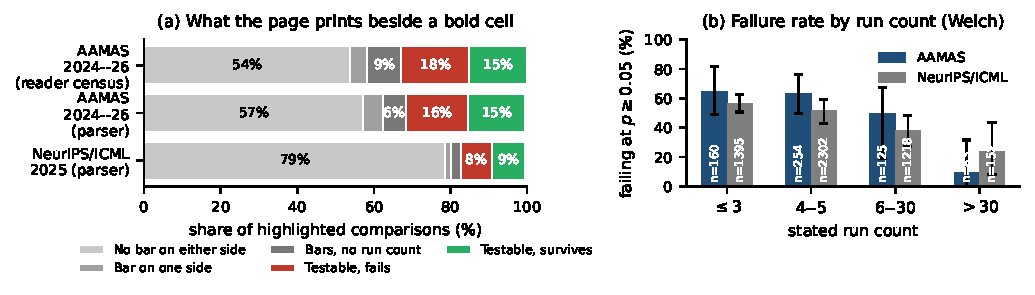
\includegraphics[width=0.92\textwidth]{fig_census}
\caption{(a) What the page prints beside a bold cell, in AAMAS 2024--2026
and in NeurIPS/ICML 2025 (all pages), as a share of the highlighted
comparisons the parser reads. (b) The share of testable comparisons failing
Welch's $t$ at the stated run count, by run count, with 95\% cluster
bootstrap intervals over papers; $n$ is the number of comparisons in the
band.}
\label{fig:census}
\end{figure*}

\begin{table*}[t]
\caption{The census. Highlighted comparisons in the AAMAS main track
2024--2026 as the image-based reader lists them on every caption page and
as the frozen parser reads them, and the parser on NeurIPS/ICML 2025 on all
pages and on main-text pages only, under one definition. Intervals are 95\%
cluster bootstraps over papers. ``$\pm$ cell'': the paper prints a $\pm$
value in a table; ``anywhere'': a $\pm$ or parenthesised cell, or a figure
caption naming a deviation, interval or band. Every reader group whose
bold cell is not the better value in its stated direction, or ties its
rival, is dropped as the parser's rules drop it, so the instruments share
one unit. ``Testable'' takes the run count from anywhere in the paper;
the caption-or-page reading is the sub-row.}
\label{tab:census}
\centering
\small
\setlength{\tabcolsep}{7pt}
\begin{tabular}{@{}lrrrr@{}}
\toprule
 & AAMAS reader & AAMAS parser & ML 2025 & ML main text \\
\midrule
Papers & \nAPapers{} & \nAPapers{} & \nMlPapers{} & \nMlPapers{} \\
Papers with a $\pm$ cell & -- & \nAPctPapersErr{} & \nMlPctPapersErr{} & \nMlMainPapersErr{} \\
Papers with uncertainty anywhere & -- & \nUaAnywhere{} & -- & -- \\
Papers stating a run count & -- & \nAPctPapersRuns{} & \nMlPctPapersRuns{} & -- \\
Median stated run count & -- & \nAMedianRuns{} & \nMlMedianRuns{} & -- \\
Highlighted comparisons & \nCzGroups{} & \nAComparisons{} & \nMlComparisons{} & \nMlMainComparisons{} \\
Papers holding them & \nCzPapersWithGroups{} & \nClaimPapers{} & -- & -- \\
No bar on either side & \nCzNeitherCi{} & \nAPctNeitherCi{} & \nMlPctNeitherCi{} & \nMlMainNeither{} \\
Bar on one side only & \nCzOneSide{} & \nAPctOneSide{} & -- & -- \\
Bars but no run count & \nCzBarsNoN{} & \nAPctNoN{} & -- & -- \\
Testable (run count from anywhere in the paper) & \nCzTestableCi{} & \nAPctTestableCi{} & \nMlPctTestableCi{} & \nMlMainTestable{} \\
\quad run count from caption or page only & -- & \nSpanCaptionOrPageTestable{} & -- & -- \\
\quad papers holding them & \nCzTestablePapers{} & \nAPapersTestable{} & \nMlTestablePapers{} & \nMlMainTestablePapers{} \\
\quad tested (values readable) & \nCzReaderFailN{} & \nANTestable{} & -- & -- \\
\quad of which fail, Welch & \nCzReaderFail{} & \nAPctFailCi{} & \nMlPctFailCi{} & \nMlMainFail{} \\
\quad fail after Holm & -- & \nAPctFailHolmCi{} & \nMlPctFailHolmCi{} & \nMlMainFailHolm{} \\
\bottomrule
\end{tabular}
\end{table*}

Table~\ref{tab:census} and Figure~\ref{fig:census}a are the census, taken
twice. The image-based reader (Section~\ref{sec:instrument} gives its
protocol) read every one of the \nCzPagesDrawn{} pages on which the parser
detected a table caption, from \nCzPapersDrawn{} of the \nAPapers{}
papers; \nCzPagesRead{} returned a valid listing (fifteen of the densest
at a lower reasoning setting, checked in the supplement), and an empty
listing cannot be told from a page without groups, which
Section~\ref{sec:instrument} measures. It listed \nCzTables{} results
tables of which \nCzTablesWithBar{} print any bar, and in them
\nCzGroups{} rows or columns with exactly one bold cell, from
\nCzPapersWithGroups{} papers, after dropping the groups whose bold cell
is not the better value or ties its rival, the rule the parser applies.
Of those, \nCzNeither{} carry no error bar
on either side (\nCzNeitherCi{} resampling papers), \nCzOneSide{} a bar on
one side only, \nCzBarsNoN{} bars but no run count, and \nCzTestable{} can
be tested with a run count from anywhere in the paper (\nCzTestableCi{};
the parser's share with the count restricted to the caption or the
table's page is \nSpanCaptionOrPageTestable{}, to the caption alone
\nStrictTestable{}), of which \nCzReaderFailN{} from
\nCzReaderFailPapers{} papers have readable values. The
parser, on the whole corpus, reads \nAComparisons{} comparisons in
\nATablesYielding{} tables: \nAPctNeither{} bar-less (\nAPctNeitherCi{}),
\nAPctOneSide{} one-sided, \nAPctNoN{} with bars but no run count anywhere
in the paper, and \nAPctTestable{} testable (\nAPctTestableCi{}). The
headline shares agree to within their intervals, but partly as a mixture:
on the \nCzPipeMatchedGroups{} comparisons both instruments list the
bar-less share is \nCzMatchedNeither{} by the reader and
\nCzPipeMatchedNeither{} by the parser, the \nCzReaderUnmatchedGroups{}
groups only the reader lists are \nCzUnmatchedNeither{} bar-less, and the
\nCzPipeUnconfirmedN{} comparisons only the parser lists are
\nCzPipeUnconfirmedNeither{} bar-less. Of those, \nEcNoneComparisons{} sit
on \nEcNonePages{} pages the reader read as results tables whose bold
marks no single winner per line (\nEcNoneNeither{} bar-less,
\nEcNoneTestable{} testable), the own-row and block-cut tables the
parser's rules keep and the census protocol does not, and
\nEcNotableComparisons{} on \nEcNotablePages{} pages it read as holding
no results table. So each headline errs in its own direction and the
matched core is the cross-instrument result.
Intervals resample papers because comparisons come in clusters (on the
parser's testable set, \nAMeanCluster{} per paper, design effect
\nADesignEffect{}, effective sample \nANEff{}); every interval on a share
of comparisons in this section and the next is a cluster bootstrap over
papers, and the agreement figures of Section~\ref{sec:instrument} carry
Wilson intervals over items or resample pages, as marked. The parser's \nANTestable{}
testable comparisons come from \nAPapersTestable{} papers, ten of which
hold \nTopTenPapersShare{} of them; the largest, \nLargestN{} comparisons
at \nLargestRuns{} runs failing at \nLargestFail{}, is a data-pricing
paper the classifier labelled game theory. The reader's \nCzReaderFailN{}
come from \nCzReaderFailPapers{} papers. Those are the populations the
failure rates of Section~\ref{sec:support} describe.

\paragraph{Against the mainstream.} On the main text of the 2025 NeurIPS and
ICML sample the same parser finds \nMlMainNeither{} bar-less and
\nMlMainTestable{} testable (\nMlPctNeither{} and \nMlPctTestable{} with
appendices). At the level of the paper the venues look alike:
\nAPctPapersErr{} of AAMAS papers print a $\pm$ cell in a table,
\nMlMainPapersErr{} of mainstream papers do so in their main text
(\nMlPctPapersErr{} with appendices), and the median stated run count is
\nAMedianRuns{} in both. The gap is in who prints the tables that make
claims. The highlighted comparisons of AAMAS come from a narrow slice of
the proceedings:
Table~\ref{tab:community} shows that the learning community holds most of
them and prints a deviation beside about half of them, against a fifth in
the mainstream, while the
game-theoretic and social-choice papers, \nCGameTheorySocialChoicePapers{}
of the \nAPapers{}, rarely mark a winner in a table at all, and the
LLM-agent papers that do mark one print bars as seldom as the mainstream.
The mainstream sample is dominated by leaderboard tables of benchmark
scores, where bars are rarest. The comparison that does not depend on the
parser is the one the image-based readers make with nothing marked, and
both readers read both venues. The census reader: \nCzNeitherCi{}
bar-less and \nCzTestableCi{} testable over every AAMAS caption page,
against \nMsNeitherCi{} and \nMsTestableCi{} on the \nMsPages{} random
mainstream pages of the concurrent study. The first reader: on a pilot of
\nPagesRead{} random AAMAS caption pages, \nPagesReaderNeither{} bar-less
and \nPagesReaderTestable{} testable, against \nScReaderNeither{} and
\nScReaderTestable{} on \nScPages{} of the same mainstream pages. The
venues separate on bars under either reader; on testability the pilot is
too small to say, and the census settles it.
On the \nMsCrossSharedPages{} mainstream pages both readers list groups,
their bar-less shares are \nMsCrossSharedFirstNeither{} and
\nMsCrossSharedSecondNeither{}, and they agree on the bar-less verdict for
\nMsCrossSharedNeitherAgreePct{} of the \nMsCrossSharedMatched{} groups
both list; they differ on which groups can be tested, failing
\nMsCrossSharedFailFirst{} of \nMsCrossSharedTestedFirst{} and
\nMsCrossSharedFailSecond{} of \nMsCrossSharedTestedSecond{} there.

\paragraph{By year.} Failure rates of \nAFailTwentyFourCi{},
\nAFailTwentyFiveCi{} and \nAFailTwentySixCi{} in 2024, 2025 and 2026,
and bar-less shares of \nANeitherTwentyFour{}, \nANeitherTwentyFive{} and
\nANeitherTwentySix{}, have overlapping intervals and no monotone order;
three years cannot separate a trend from the papers that happened to be
accepted.

\begin{table}[t]
\caption{By community, from a language-model reading of title and first page.
``Claim'' is the share of papers with at least one highlighted comparison;
``Bar'' the share with a $\pm$ cell in a table; ``T.\,papers'' the number of
papers holding a testable comparison; the failure rate is over testable
comparisons and is omitted where fewer than twenty exist or fewer than five
papers hold them.}
\label{tab:community}
\footnotesize
\setlength{\tabcolsep}{2.6pt}
\begin{tabular}{@{}lrrrrrrr@{}}
\toprule
Community & Papers & Claim & Bar & No bar & Testable & T.\,papers & Fail \\
\midrule
Learning & \nCLearningPapers{} & \nCLearningClaimPapers{} & \nCLearningPapersErr{} & \nCLearningNeither{} & \nCLearningTestable{} & \nCLearningTestablePapers{} & \nCLearningFail{} \\
Game theory, social choice & \nCGameTheorySocialChoicePapers{} & \nCGameTheorySocialChoiceClaimPapers{} & \nCGameTheorySocialChoicePapersErr{} & \nCGameTheorySocialChoiceNeither{} & \nCGameTheorySocialChoiceTestable{} & \nCGameTheorySocialChoiceTestablePapers{} & \nCGameTheorySocialChoiceFail{} \\
LLM agents & \nCLlmAgentsPapers{} & \nCLlmAgentsClaimPapers{} & \nCLlmAgentsPapersErr{} & \nCLlmAgentsNeither{} & \nCLlmAgentsTestable{} & \nCLlmAgentsTestablePapers{} & \nCLlmAgentsFail{} \\
Simulation & \nCSimulationPapers{} & \nCSimulationClaimPapers{} & \nCSimulationPapersErr{} & \nCSimulationNeither{} & \nCSimulationTestable{} & \nCSimulationTestablePapers{} & \nCSimulationFail{} \\
Planning, search & \nCPlanningSearchPapers{} & \nCPlanningSearchClaimPapers{} & \nCPlanningSearchPapersErr{} & \nCPlanningSearchNeither{} & \nCPlanningSearchTestable{} & \nCPlanningSearchTestablePapers{} & \nCPlanningSearchFail{} \\
Reasoning, norms & \nCReasoningNormsPapers{} & \nCReasoningNormsClaimPapers{} & \nCReasoningNormsPapersErr{} & \nCReasoningNormsNeither{} & \nCReasoningNormsTestable{} & \nCReasoningNormsTestablePapers{} & \nCReasoningNormsFail{} \\
Robotics, HAI & \nCRoboticsHaiPapers{} & \nCRoboticsHaiClaimPapers{} & \nCRoboticsHaiPapersErr{} & \nCRoboticsHaiNeither{} & \nCRoboticsHaiTestable{} & \nCRoboticsHaiTestablePapers{} & \nCRoboticsHaiFail{} \\
Other & \nCOtherPapers{} & \nCOtherClaimPapers{} & \nCOtherPapersErr{} & \nCOtherNeither{} & \nCOtherTestable{} & \nCOtherTestablePapers{} & \nCOtherFail{} \\
\bottomrule
\end{tabular}
\end{table}

\paragraph{By community.} Table~\ref{tab:community} splits the corpus by the
label a model gave each paper. The learning papers contribute
\nCLearningComparisons{} of the \nAComparisons{} comparisons and
\nCLearningNTestable{} of the \nANTestable{} testable ones, failing at
\nCLearningFail{}; the LLM-agent papers are the other large source
(\nCLlmAgentsComparisons{}) and the one that looks most like the
mainstream, \nCLlmAgentsNeither{} of their comparisons carrying no bar;
the game-theoretic and social-choice papers, \nCGameTheorySocialChoicePapers{}
of the corpus, mark a winner in \nCGameTheorySocialChoiceClaimPapers{}
of papers. The audit that follows is, in effect, an audit of how
multi-agent learning (single-agent RL included, as Table~\ref{tab:env}
shows) and agentic-LLM work is reported at AAMAS; the other communities
are counted, but their claims live in theorems and figures the parser
does not read.

\section{What the printed evidence supports}
\label{sec:support}

Of the \nANTestable{} testable comparisons, from \nAPapersTestable{} papers,
\nAPctFail{} are not distinguishable from zero at the stated run count
(\nAPctFailCi{} over papers): Welch's $t$ on the \nWelchN{} with a run
count, \nWelchFail{} of which fail, and a normal-limit $z$ on the \nZN{}
standard errors and intervals that need none, \nZFail{} of which fail;
\nAPctFailHolm{} fail after Holm's correction within the table. From the
reader's own values on the census, \nCzReaderFail{} of its
\nCzReaderFailN{} testable comparisons fail. On the \nCzShared{}
comparisons both instruments test the verdicts agree on \nCzSharedAgree{}:
the parser fails \nCzSharedPipeFailPct{} of them and the reader
\nCzSharedReaderFailPct{}, the parser failing where the reader survives on
\nCzSharedPipeFailsReaderSurvives{} and the reverse on
\nCzSharedReaderFailsPipeSurvives{}, mostly a different run count
accepted; the reader's higher rate over its \nCzReaderFailN{} comes from
the \nCzReaderOnlyN{} comparisons the parser does not test, which fail at
\nCzReaderOnlyFailPct{}. With the paper as the unit, the median paper
fails \nPpMedian{} of its testable comparisons (quartiles \nPpQOne{} and
\nPpQThree{}), the mean of the paper rates is \nPpMean{}, and
\nPpAllFail{} of the \nPpPapers{} papers fail every one; the distribution
is wide with both ends occupied, and the pooled rate is a spread across
most papers, not one paper's habit. Where
a caption itself asserts superiority (outperforms, significantly, surpasses,
state of the art), which \nCapAssertingPapers{} papers' captions do for
\nCapAssertingN{} testable comparisons, \nCapAssertingFail{} fail; where
the caption only describes the table, \nCapDescribingFail{} of
\nCapDescribingN{} do. Bold by convention and bold with a claim behind it
fare alike; on few papers, the asserted claims are if anything less
reproducible from the page, which does not contradict a test the authors
ran on data the page does not print. The median relative gap among the failing
comparisons is \nAGapFail{}, among the surviving ones \nAGapPass{}. A
two-sample $z$ on the same comparisons, each printed deviation taken as
exact, fails \nSpanZTwoSidedFail{}. On the mainstream sample the
corresponding rates are \nMlMainFail{} on main-text pages and \nMlPctFail{}
on all pages, but the pooled pair mixes RL tables with leaderboard tables.
Within the RL environment families the captions name (the same patterns
on both corpora), AAMAS fails at \nFmAamasRlFail{} \nFmAamasRlFailCi{} on
\nFmAamasRlN{} comparisons from \nFmAamasRlPapers{} papers against the
mainstream's \nFmMlRlFail{} \nFmMlRlFailCi{} (\nFmMlRlN{} from
\nFmMlRlPapers{}); outside them AAMAS fails at \nFmAamasRestFail{}
\nFmAamasRestFailCi{} against \nFmMlRestFail{} \nFmMlRestFailCi{}. The
intervals over two dozen papers overlap; the direction is that the RL
tables of AAMAS resolve their claims less often than the mainstream's, and
its other tables more often.

\paragraph{Seeds.} Figure~\ref{fig:census}b splits the failure rate by
run count. At three seeds or fewer (\nRunsLeThreeN{} comparisons from
\nRunsLeThreePapers{} papers) \nRunsLeThreeFailCi{} fail; at four or five
(\nRunsFourToFiveN{} from \nRunsFourToFivePapers{})
\nRunsFourToFiveFailCi{}; at six to thirty (\nRunsSixToThirtyN{} from
\nRunsSixToThirtyPapers{}) \nRunsSixToThirtyFailCi{}; above thirty
(\nRunsGtThirtyN{} from \nRunsGtThirtyPapers{}) \nRunsGtThirtyFailCi{}.
The first three intervals, over papers, overlap; the well-powered band
separates from the two few-seed bands and overlaps the six-to-thirty
band, and the protocol reading of
Section~\ref{sec:protocol} puts the deviation over those runs in
\nBignSdOverSeedsPapers{} of its \nBignPapers{} papers
(\nBignSdOverSeedsComparisons{} comparisons) and over evaluation episodes
in \nBignSdOverEpisodesPapers{} (\nBignSdOverEpisodesComparisons{}).
Part of the rest is the arithmetic of the $t$ distribution. The largest gap
among the \nExNThreeSeedFailing{} three-seed win-rate comparisons that fail
is \nExWinner{} against \nExRunner{} points, with printed deviations of
\nExWinnerSd{} and \nExRunnerSd{}: a gap of \nExGap{} points,
\nExRelativeGap{} of the rival, gives $t = \nExT{}$ on \nExDf{} degrees of
freedom and $p = \nExP{}$. Three seeds cannot certify an eleven-point win
rate difference when the seeds themselves differ by eight. The same paper
states five seeds in one place and three in another; the smallest-count
rule takes three, both readers took \nExReaderN{}, under which
$t = \nExReaderT{}$ on \nExReaderDf{} degrees of freedom and
$p = \nExReaderP{}$, and the caption does not settle it. The count comes
from outside the caption and the table's page for \nSpanRunsFromPaperN{}
of the \nANTestable{} testable comparisons (\nSpanRunsFromPaperPapers{}
papers), which fail at \nSpanRunsFromPaperFail{}. Few seeds resolving
little is what the seed-count literature predicted
\cite{colas2018how,agarwal2021deep} and the reason
\citet{gorsane2022towards} asked for ten.

\paragraph{Environments.} Table~\ref{tab:env} in Section~\ref{sec:protocol}
gives the failure rate by environment family; the MuJoCo, D4RL and
control tables, which multi-agent papers share with single-agent RL, fail
most often, and every family rests on a handful of papers whose rates are
theirs, not the environments'.

\begin{table}[t]
\caption{The span of the failure rate across conventions the papers leave
unstated and artefacts the reference set exposed. Each row changes one
reading of the page and keeps the rest; $n$ is the number of testable
comparisons under that reading, $P$ the papers they come from, and the
interval a 95\% cluster bootstrap over papers.}
\label{tab:span}
\footnotesize
\setlength{\tabcolsep}{3pt}
\begin{tabular}{@{}lrrl@{}}
\toprule
Reading & $n$ & $P$ & Fail [95\% CI] \\
\midrule
Welch's $t$ at the stated run count (reported) & \nSpanAsReportedN{} & \nSpanAsReportedPapers{} & \nSpanAsReportedFail{} \nSpanAsReportedFailCi{} \\
Two-sample $z$, deviations exact & \nSpanZTwoSidedN{} & \nSpanZTwoSidedPapers{} & \nSpanZTwoSidedFail{} \nSpanZTwoSidedFailCi{} \\
One-sided & \nSpanOneSidedN{} & \nSpanOneSidedPapers{} & \nSpanOneSidedFail{} \nSpanOneSidedFailCi{} \\
Printed deviation read as a population SD & \nDdofN{} & \nSpanAsReportedPapers{} & \nDdofFail{} \\
Holm within table & \nSpanAsReportedN{} & \nSpanAsReportedPapers{} & \nSpanAsReportedFailHolm{} \\
Holm within paper & \nSpanHolmFamilyPaperN{} & \nSpanHolmFamilyPaperPapers{} & \nSpanHolmFamilyPaperFailHolm{} \\
Unlabelled bars read as standard errors & \nSpanUnlabelledAsSemN{} & \nSpanUnlabelledAsSemPapers{} & \nSpanUnlabelledAsSemFail{} \nSpanUnlabelledAsSemFailCi{} \\
Labelled bars only & \nSpanLabelledOnlyN{} & \nSpanLabelledOnlyPapers{} & \nSpanLabelledOnlyFail{} \nSpanLabelledOnlyFailCi{} \\
Run count from the caption only & \nSpanCaptionOnlyN{} & \nSpanCaptionOnlyPapers{} & \nSpanCaptionOnlyFail{} \nSpanCaptionOnlyFailCi{} \\
Run count from caption or page & \nSpanCaptionOrPageN{} & \nSpanCaptionOrPagePapers{} & \nSpanCaptionOrPageFail{} \nSpanCaptionOrPageFailCi{} \\
Methods paired, $\rho = 0.5$ & \nSpanRhoHalfN{} & \nSpanRhoHalfPapers{} & \nSpanRhoHalfFail{} \nSpanRhoHalfFailCi{} \\
Methods paired, $\rho = 0.9$ & \nSpanRhoNineTenthsN{} & \nSpanRhoNineTenthsPapers{} & \nSpanRhoNineTenthsFail{} \nSpanRhoNineTenthsFailCi{} \\
Unlabelled bars typed by the protocol reading & \nTuN{} & \nTuPapers{} & \nTuFail{} \\
Run counts of thirty or fewer only & \nRBigNRemovedTestableN{} & \nRBigNRemovedTestablePapers{} & \nRBigNRemovedFail{} \nRBigNRemovedFailCi{} \\
Captions saying median or IQM removed & \nRMedianRemovedTestableN{} & \nRMedianRemovedTestablePapers{} & \nRMedianRemovedFail{} \nRMedianRemovedFailCi{} \\
Shared set, at the reader's run count & \nCzShared{} & -- & \nCzSharedReaderFailPct{} \\
Duplicate table records removed & \nRDupRemovedTestableN{} & \nRDupRemovedTestablePapers{} & \nRDupRemovedFail{} \nRDupRemovedFailCi{} \\
Merged side-by-side tables removed & \nRMergedRemovedTestableN{} & \nRMergedRemovedTestablePapers{} & \nRMergedRemovedFail{} \nRMergedRemovedFailCi{} \\
Exact-copy comparisons removed & \nRCopiesRemovedTestableN{} & \nRCopiesRemovedTestablePapers{} & \nRCopiesRemovedFail{} \nRCopiesRemovedFailCi{} \\
All three artefacts removed & \nRAllArtefactsRemovedTestableN{} & \nRAllArtefactsRemovedTestablePapers{} & \nRAllArtefactsRemovedFail{} \nRAllArtefactsRemovedFailCi{} \\
Tables that bold one whole line removed & \nROwnRowRemovedTestableN{} & \nROwnRowRemovedTestablePapers{} & \nROwnRowRemovedFail{} \nROwnRowRemovedFailCi{} \\
Comparisons with a zero deviation removed & \nRZeroRemovedTestableN{} & \nRZeroRemovedTestablePapers{} & \nRZeroRemovedFail{} \nRZeroRemovedFailCi{} \\
Copied rivals removed, both extremes & \nCopiedRemovedN{} & -- & \nFailCopiedRemovedLow{}--\nFailCopiedRemovedHigh{} \\
\bottomrule
\end{tabular}
\end{table}

\paragraph{Conventions.} Table~\ref{tab:span} moves one reading at a time.
The run count matters most for how much can be tested: captions alone
leave \nStrictN{} comparisons testable (\nStrictTestable{} of the corpus)
at \nStrictFail{}, and a count from anywhere in the paper, which the
headline uses, more than doubles the set at almost the same rate. What
the bar means matters most for the rate:
\nBarsUnlabelledPct{} of the bars that reach the test are unlabelled, and
reading them as standard errors rather than deviations moves their failure
rate from \nBarsAsStdFail{} to \nBarsAsSemFail{}; the labelled bars alone
fail at \nBarsLabelledFail{}. The reference set puts the parser's
agreement with a reader on the raw kind of bar at \nGDispTypeFrac{} and
on the run count at \nGNRunsFrac{}, its two weakest fields, and at
\nGDispTreatmentFrac{} on the kind as the test uses it; typing the
unlabelled bars by what the protocol reading of Section~\ref{sec:protocol}
says their paper's deviation is gives \nTuFail{}, the evidence for the
deviation default.
\nRZeroN{} testable comparisons carry a printed deviation of zero on one
side, none on both; \nRZeroFail{} of them fail, and the rate without them
is \nRZeroRemovedFail{}. \nRBigNOnlyN{} comparisons from
\nRBigNOnlyPapers{} papers carry a run count above thirty, the
well-powered papers; they fail at \nRBigNOnlyFail{}, and the rate among
papers stating thirty or fewer is \nRBigNRemovedFail{}. Across the
full-population rows the rate spans \nSpanLo{} to \nSpanHi{}, as wide as
the sampling interval: the pages do not say enough to pin down their own
claims.

\paragraph{Artefacts and strata removed.} The last rows filter the parser's
output by what the reference set of Section~\ref{sec:instrument} found:
\nRDupOnlyN{} comparisons from duplicated table records, which fail at
\nRDupOnlyFail{}, the signature of a rival taken from the wrong record;
\nRMergedTables{} tables that carry two captions in one, two tables set
side by side that the window merged; and \nRCopiesOnlyN{} comparisons in
\nRCopiesPapers{} papers that are exact copies of another on the same
page under a different table number, which inflate the concentration
statistics more than the rates and which Section~\ref{sec:protocol}
leaves out. With all three removed the corpus is
\nRAllArtefactsRemovedN{} comparisons, \nRAllArtefactsRemovedNeither{}
bar-less, \nRAllArtefactsRemovedTestable{} testable and
\nRAllArtefactsRemovedFail{} failing. The frozen headline keeps them in,
because the filters are post-hoc exclusions the reference set exposed;
Table~\ref{tab:span} prints the rate without them, and it is the higher
one. Ablation tables, where bold marks the full model rather than a
winner, and tables that bold one whole line move the rate little;
\nGRivalCopied{} of the reference set's rivals carry a citation, dagger
or ``reported in'' marker, a number copied from another paper, and
removing every such comparison at either extreme bounds the rate between
\nFailCopiedRemovedLow{} and \nFailCopiedRemovedHigh{}.

The \nCcCitingPapers{} papers citing the evaluation-methodology literature
print bars and run counts more often and fail no less often (supplement).

\section{The resolution of the evaluation protocol}
\label{sec:protocol}

A win rate or a success rate is a proportion, and a proportion measured over
$K$ episodes has a standard error of $\sqrt{p(1-p)/K}$ whether or not anyone
prints it. Two rates measured over $K$ independent episodes each cannot be
told apart when their gap is below the interval a two-proportion test
gives at $p < 0.05$, in the normal limit
$1.96\,\sqrt{p_1(1-p_1)/K + p_2(1-p_2)/K}$ and, as computed here,
Newcombe's interval built from the Wilson limits of each arm, which
behaves at the boundary where the Wald term collapses and where StarCraft
maps won on every episode sit; no bold face changes that. This resolution
is a property of the protocol, and it is the one quantity in this paper
that can be computed for a bar-less comparison from what the page prints,
provided the page prints $K$. Where $K$ and the seeds are both stated it
is a floor under the noise, since the variance between seeds sits on top
of the binomial term; where the seeds are not stated it is an assumed
resolution, not a bound; and it takes the two arms as independent, so
where both methods run on the same episodes or the same fixed instance
set the noise of the difference is smaller and the term is a bound only
under independence.

\paragraph{What the papers state.} A language model read the first
60,000 characters of every learning-labelled paper and every paper holding
a rate or a testable comparison, \nPtwoPapers{} in all
(\nPtwoAgentsSingle{} of them controlling a single agent), and reported $K$, the seeds,
whether $K$ counts sampled episodes or a fixed set of instances, the
environments, the codebase, whether the compared methods share evaluation
episodes, and what the printed deviation is over; the prompt and every
answer, with the sentences quoted, are released. It finds $K$ in
\nPtwoWithK{} of the \nPtwoPapers{} papers (\nPtwoWithKPct{}) and a seed
count in \nPtwoWithSeeds{} (\nPtwoWithSeedsPct{}); regular expressions
over the same texts agree with it on the value of $K$ in
\nPtwoRegexAgreeK{} of the \nPtwoRegexBothK{} papers where both find one,
and no human read any of the papers. The right
denominator for the question is narrower: \nPtwoRatePapers{} papers
highlight a rate at all, and the model finds $K$ in
\nPtwoRatePapersWithK{} of them, the patterns in
\nPtwoRatePapersRegexK{}. \nPtwoRatePapersSmac{} of the rate papers
evaluate on SMAC or SMACv2, whose PyMARL default evaluates over 32
episodes; imputing that where the paper states no $K$ raises the papers
with one to \nPtwoRatePapersWithKInherited{}. The
model reads the printed deviation as one over seeds in
\nPtwoSdOverSeeds{} papers, over pooled evaluation episodes in
\nPtwoSdOverEpisodes{}, a standard error in \nPtwoSdOverSe{}, an interval
in \nPtwoSdOverCi{} and unstated in \nPtwoSdOverUnsure{}; the compared methods share evaluation
episodes in \nPtwoSharesEvalYes{} papers and are stated to differ in
\nPtwoSharesEvalNo{}. Table~\ref{tab:env} gives the protocol by
environment family.

\begin{table}[t]
\caption{The evaluation protocol by environment family, from the model's
reading of \nPtwoPapers{} papers: papers, the share stating $K$ and the
modal $K$, the share stating seeds and the modal count, the gap in points
two rates near 50\% can resolve at the modal $K \times S$, and the
parser's failure rate on the testable comparisons of those papers, with
the comparisons and papers ($n$/$P$) it rests on. A mode is printed with
the papers behind it and only where at least two agree; the resolution
only where the family's headline metric is a rate; the failure rate only
on twenty comparisons from five papers, as in Table~\ref{tab:community}.
A paper with several environments counts in each; the last row holds the
papers in none of the families. MP is Melting Pot, GRF Google Research
Football.}
\label{tab:env}
\scriptsize
\setlength{\tabcolsep}{2pt}
\begin{tabular}{@{}lrrrrrrrr@{}}
\toprule
Environment & Papers & $K$ & mode & Seeds & mode & Res. & Fail & $n$/$P$ \\
\midrule
SMAC, SMACv2 & \nPenvSmacSmacvPapers{} & \nPenvSmacSmacvStateK{} & \nPenvSmacSmacvModalK{} & \nPenvSmacSmacvStateSeeds{} & \nPenvSmacSmacvModalSeeds{} & \nPenvSmacSmacvResolution{} & \nPenvSmacSmacvFail{} & \nPenvSmacSmacvTestable{}/\nPenvSmacSmacvTestablePapers{} \\
GRF & \nPenvGoogleResearchFootballPapers{} & \nPenvGoogleResearchFootballStateK{} & \nPenvGoogleResearchFootballModalK{} & \nPenvGoogleResearchFootballStateSeeds{} & \nPenvGoogleResearchFootballModalSeeds{} & \nPenvGoogleResearchFootballResolution{} & \nPenvGoogleResearchFootballFail{} & \nPenvGoogleResearchFootballTestable{}/\nPenvGoogleResearchFootballTestablePapers{} \\
MPE & \nPenvMpePapers{} & \nPenvMpeStateK{} & \nPenvMpeModalK{} & \nPenvMpeStateSeeds{} & \nPenvMpeModalSeeds{} & \nPenvMpeResolution{} & \nPenvMpeFail{} & \nPenvMpeTestable{}/\nPenvMpeTestablePapers{} \\
MaMuJoCo & \nPenvMamujocoPapers{} & \nPenvMamujocoStateK{} & \nPenvMamujocoModalK{} & \nPenvMamujocoStateSeeds{} & \nPenvMamujocoModalSeeds{} & \nPenvMamujocoResolution{} & \nPenvMamujocoFail{} & \nPenvMamujocoTestable{}/\nPenvMamujocoTestablePapers{} \\
Hanabi, Overcooked, MP & \nPenvHanabiOvercookedMeltingPotPapers{} & \nPenvHanabiOvercookedMeltingPotStateK{} & \nPenvHanabiOvercookedMeltingPotModalK{} & \nPenvHanabiOvercookedMeltingPotStateSeeds{} & \nPenvHanabiOvercookedMeltingPotModalSeeds{} & \nPenvHanabiOvercookedMeltingPotResolution{} & \nPenvHanabiOvercookedMeltingPotFail{} & \nPenvHanabiOvercookedMeltingPotTestable{}/\nPenvHanabiOvercookedMeltingPotTestablePapers{} \\
1-agent MuJoCo, DMC, D4RL & \nPenvSingleagentMujocoDmcDrlPapers{} & \nPenvSingleagentMujocoDmcDrlStateK{} & \nPenvSingleagentMujocoDmcDrlModalK{} & \nPenvSingleagentMujocoDmcDrlStateSeeds{} & \nPenvSingleagentMujocoDmcDrlModalSeeds{} & \nPenvSingleagentMujocoDmcDrlResolution{} & \nPenvSingleagentMujocoDmcDrlFail{} & \nPenvSingleagentMujocoDmcDrlTestable{}/\nPenvSingleagentMujocoDmcDrlTestablePapers{} \\
Atari & \nPenvAtariPapers{} & \nPenvAtariStateK{} & \nPenvAtariModalK{} & \nPenvAtariStateSeeds{} & \nPenvAtariModalSeeds{} & \nPenvAtariResolution{} & \nPenvAtariFail{} & \nPenvAtariTestable{}/\nPenvAtariTestablePapers{} \\
Gridworlds & \nPenvGridworldsPapers{} & \nPenvGridworldsStateK{} & \nPenvGridworldsModalK{} & \nPenvGridworldsStateSeeds{} & \nPenvGridworldsModalSeeds{} & \nPenvGridworldsResolution{} & \nPenvGridworldsFail{} & \nPenvGridworldsTestable{}/\nPenvGridworldsTestablePapers{} \\
Traffic & \nPenvTrafficPapers{} & \nPenvTrafficStateK{} & \nPenvTrafficModalK{} & \nPenvTrafficStateSeeds{} & \nPenvTrafficModalSeeds{} & \nPenvTrafficResolution{} & \nPenvTrafficFail{} & \nPenvTrafficTestable{}/\nPenvTrafficTestablePapers{} \\
LLM benchmarks & \nPenvLlmBenchmarksPapers{} & \nPenvLlmBenchmarksStateK{} & \nPenvLlmBenchmarksModalK{} & \nPenvLlmBenchmarksStateSeeds{} & \nPenvLlmBenchmarksModalSeeds{} & \nPenvLlmBenchmarksResolution{} & \nPenvLlmBenchmarksFail{} & \nPenvLlmBenchmarksTestable{}/\nPenvLlmBenchmarksTestablePapers{} \\
Matrix games & \nPenvMatrixAndNormalformGamesPapers{} & \nPenvMatrixAndNormalformGamesStateK{} & \nPenvMatrixAndNormalformGamesModalK{} & \nPenvMatrixAndNormalformGamesStateSeeds{} & \nPenvMatrixAndNormalformGamesModalSeeds{} & \nPenvMatrixAndNormalformGamesResolution{} & \nPenvMatrixAndNormalformGamesFail{} & \nPenvMatrixAndNormalformGamesTestable{}/\nPenvMatrixAndNormalformGamesTestablePapers{} \\
None of these & \nPenvOtherOrNoneOfThesePapers{} & \nPenvOtherOrNoneOfTheseStateK{} & \nPenvOtherOrNoneOfTheseModalK{} & \nPenvOtherOrNoneOfTheseStateSeeds{} & \nPenvOtherOrNoneOfTheseModalSeeds{} & \nPenvOtherOrNoneOfTheseResolution{} & \nPenvOtherOrNoneOfTheseFail{} & \nPenvOtherOrNoneOfTheseTestable{}/\nPenvOtherOrNoneOfTheseTestablePapers{} \\
\bottomrule
\end{tabular}
\end{table}

\paragraph{Which comparisons are rates.} A comparison counts as a rate
when its table's caption or header names a win, winning, success, solved
or completion rate, the record is anchored on a caption beginning
``Table'', the bold marks the higher value, the group's own row label and
column header (read from the PDF text layer around the parser's
coordinates) name no other metric, and its values sit on the table's
scale: \nRfKept{} of \nRfTableNamesARate{} candidates from
\nRfKeptPapers{} papers remain (\nPtwoResTypedRateLike{} with exact copies
removed; the supplement counts each rule). An earlier table-level filter
admitted the time, cost and return columns of tables whose caption named
a success rate, which a reviewer caught; no human checked the survivors.

\paragraph{Gaps below resolution.} \nPtwoResTypedN{} of those
comparisons, from the \nPtwoResTypedPapers{} papers that state $K$, can be
set against their protocol. None of those papers evaluates on StarCraft,
football or particle environments (\nPtwoKPapersMarlBench{} do) and
\nPtwoKPapersSingle{} of them control a single agent, so the measured
result is not the MARL protocol the section is named for; the StarCraft
papers enter only through the imputed reading below. Taking $K$ episodes
per seed times the stated seeds where $K$ counts sampled episodes, $K$
alone where it counts a fixed instance set (\nPtwoRatePapersFixed{} of
the \nPtwoRatePapers{} rate papers, whose seeds re-run the same items),
$K$ times the folds where a paper cross-validates over disjoint items
(one paper, \nPtwoResTypedCvFolds{} comparisons), and one seed where none
is stated for sampled episodes, \nPtwoResTypedBelow{} of the gaps fall
below the resolution of the protocol that produced them
(\nPtwoResTypedBelowPaperCi{} over \nPtwoResTypedPapers{} papers,
indicative only at that count; the supplement lists every paper). A rate
over $n$ trials is a multiple of $1/n$, which is a free check on every
$K$ the model read: \nPtwoResTypedLatticeConsistent{} of the
\nPtwoResTypedN{} comparisons, from \nPtwoResTypedLatticeConsistentPapers{}
papers, print values on the lattice their $n$ implies, and
\nPtwoResTypedLatticeBelowPct{} of those fall below the resolution; an
off-lattice value means a mean over runs the page does not count or a
misread $K$, and no human has read any of the eight papers to say which.
The
reading moves with the seed assumption, the fixed-instance rule held
throughout: \nPtwoSpanSeedsStatedOnlyBelow{} on the
\nPtwoSpanSeedsStatedOnlyN{} comparisons from
\nPtwoSpanSeedsStatedOnlyPapers{} papers stating both $K$ and seeds,
\nPtwoSpanSeedsStatedOrFiveBelow{} with five seeds assumed where none is
stated, \nPtwoSpanSeedsOneForAllBelow{} with $K$ alone for every
comparison, \nPtwoSpanKTimesSeedsForAllBelow{} with $K$ times seeds for
every comparison. The independence the term assumes holds for few of
them: \nPtwoResTypedSharedN{} comparisons from
\nPtwoResTypedSharedPapers{} papers evaluate the compared methods on the
same episodes or instances by the model's reading, and there the
binomial term overstates the noise of the difference; under the coarsest
paired reading the page allows, a sign test that needs six one-way
discordant instances, \nPtwoResTypedSharedPairedBelow{} of those
\nPtwoResTypedSharedN{} still fall below $6/K$. Only the
\nPtwoResTypedIndepN{} comparisons from \nPtwoResTypedIndepPapers{}
papers with independent or unstated draws are bounded by the argument,
and \nPtwoResTypedIndepBelow{} of them fall below it. With PyMARL's count
imputed to the SMAC papers that state none, an assumed $K$ and not a
floor, \nPtwoResInheritedN{} comparisons from \nPtwoResInheritedPapers{}
papers give \nPtwoResInheritedBelow{} (\nPtwoResInheritedBelowPaperCi{});
only \nPtwoResInheritedLatticeConsistent{} of them print values on the
lattice the imputed count implies, and of the
\nPtwoResInheritedWelchPass{} barred comparisons in that set that pass
Welch's $t$ on their printed deviation,
\nPtwoResInheritedWelchPassBelow{} lie below the imputed term, which
cannot hold unless the deviation is not over independent seeds or the
paper averaged more episodes than the default. The pattern-read $K$
alone gives \nResBelowPct{} on \nResWithK{} comparisons from
\nResPapers{} papers. \citet{gorsane2022towards} recorded evaluation
episode counts by hand on papers up to 2022, none of them in this corpus,
and found the same convention-driven values. So few papers cannot carry a
rate for the venue and we offer none; the finding is that the quantity
can be computed at all, that where it can it meets about half the claims
it is set against, a share that moves by tens of points with a seed
count and an independence the page does not give, and that most papers
that highlight a rate do not say over how many episodes it was measured.

\section{The parser, and how far to trust it here}
\label{sec:instrument}

\paragraph{How it reads.} The parser takes the PDF's text layer through
PyMuPDF. A table is anchored on a caption beginning ``Table $n$'', which
opens a window bounded by the caption's extent and the next caption; the
numeric cells in the window are the table, bold is read from the font
flags, and a cell's error bar is whatever follows its mean as $a \pm b$,
$a(b)$ or $a[b, c]$. Rows and columns come from the cells' coordinates,
the orientation is the axis on which most lines hold exactly one bold
cell, cut into blocks where several lines agree on a break, and the rival
is the best non-bold cell in the read direction, whatever column it sits
in. The run count is searched for in the caption, then the table's page,
then the paper, and the smallest count is taken. Every rule was fixed on
single-column NeurIPS and ICML PDFs; AAMAS papers are two-column ACM
documents with narrower tables, tables that span both columns, and body
text beside every table, so the earlier precision and recall figures do
not transfer. Table~\ref{tab:validation} collects every measurement of
what the parser and the readers do on this format; the paragraphs below
say what the table cannot.

\begin{table*}[t]
\caption{Every validation exercise, in one place. ``First'' and ``second''
are the two image-based readers (two vendors, named in the AI use
statement). Wilson intervals are over items; ``papers'' and ``pages''
intervals are cluster bootstraps. No human labelled any item: these are
agreements between instruments, not precision against a reference.}
\label{tab:validation}
\scriptsize
\centering
\setlength{\tabcolsep}{3pt}
\begin{tabular}{@{}p{2.7cm}lp{1.9cm}p{1.8cm}p{10.4cm}@{}}
\toprule
Exercise & Reader & Items & Compared with & Result \\
\midrule
Reference set, testable stratum & first & \nGTestableN{} boxed cells & parser & whole claim \nGClaimFrac{}, \nGClaim{} (Wilson), \nGClaimPaperCi{} over papers; verdict \nGVerdictFrac{} of those both test, \nGVerdictFullFrac{} of the stratum \\
Reference set, bar-less stratum & first & \nGNoBarN{} boxed cells & parser & no bar for either cell in \nGNoBarAbsentFrac{}; \nGNoBarNotTable{} items are not tables at all \\
Reference set, second reader & second & same items & parser & whole claim \nGThreeClaimFrac{}, verdict \nGThreeVerdictFrac{}, no bar \nGThreeNoBarAbsentFrac{} \\
Reference set, reader against reader & both & same items & each other & bold cell \nReadersAgreeBold{}, winner \nReadersAgreeWinner{}, runner-up \nReadersAgreeRunner{}, run count \nReadersAgreeRuns{} \\
Pilot, random caption pages & first & \nPagesRead{} pages & parser & reader lists \nPagesReaderGroups{} groups, \nPagesReaderNeither{} bar-less, \nPagesReaderTestable{} testable (\nPagesReaderFailN{} tested, \nPagesReaderFail{} fail); parser lists \nPagesReaderFoundPct{} of them \\
Census, every caption page & second & \nCzPagesRead{} pages & parser & \nCzGroups{} groups; parser lists \nCzReaderFoundPct{} of them (\nCzReaderFoundPageCi{} over pages), reader lists \nCzPipeFoundPct{} of the parser's; verdicts agree on \nCzSharedAgree{} of \nCzShared{} \\
Reader against reader, pilot pages & both & \nCcrPages{} pages & each other & \nCcrFirstGroups{} against \nCcrSecondGroups{} groups; \nCcrUnmatchedOnEmptyPages{} of the \nCcrFirstUnmatched{} unmatched first-reader groups sit on the \nCcrPagesSecondEmpty{} pages the census reader returned empty; on the \nCcrSharedPages{} pages both list, \nCcrSharedMatchedPct{} matched, bar-less \nCcrSharedFirstNeither{} against \nCcrSharedSecondNeither{}, verdicts \nCcrSharedNeitherAgreePct{} and \nCcrSharedFailAgree{} of \nCcrSharedBothTested{} \\
Empty census pages & second & \nEcPages{} pages & parser & pages holding \nEcComparisons{} parser comparisons: \nEcNonePages{} read as results tables with no single winner per line (\nEcNoneComparisons{} comparisons, \nEcNoneNeither{} bar-less), \nEcNotablePages{} as holding no results table (\nEcNotableComparisons{}) \\
Test--retest & second & \nRtPages{} pages & itself & \nRtGroupsFirst{} against \nRtGroupsSecond{} groups, \nRtMatchedCi{} of the first read matched (pages); \nRtPagesIdentical{} pages identical, \nRtPagesFirstEmpty{} and \nRtPagesSecondEmpty{} empty in one run only; bar-less verdict \nRtNeitherAgreePct{}, Welch verdict \nRtFailAgree{} of \nRtBothTested{} \\
Reasoning-effort check & second & \nRePages{} pages & itself at ``low'' & \nReMatchedCi{} of groups matched; bar-less verdict \nReNeitherAgreePct{}, Welch \nReFailAgree{} of \nReBothTested{}; bar-less share \nReNeitherFirst{} against \nReNeitherSecond{} \\
Empty listings re-read & second & \nZrPages{} pages & itself & pages on which the parser reads a comparison and the census listed nothing: \nZrPagesWithGroups{} yield groups on a second read (\nZrGroups{}, \nZrNeither{} bar-less); with them substituted the census is \nZruGroups{} groups, \nZruNeitherCi{} bar-less, \nZruTestableCi{} testable, recall \nZruRecall{} \\
Caption-less pages & second & \nNcPages{} random pages & -- & pages on which the parser detected no caption: \nNcPagesAnyTable{} hold a table of any kind (Wilson upper bound \nNcPagesAnyTableUpper{}) \\
Mainstream pages & both & \nMsPages{} pages & each other, parser & census reader \nMsNeitherCi{} bar-less, \nMsTestableCi{} testable; first reader \nScReaderNeither{}, \nScReaderTestable{}; on the \nMsCrossSharedPages{} pages both list, \nMsCrossSharedMatchedPct{} matched, verdict \nMsCrossSharedNeitherAgreePct{}; \nMsCrossPagesSecondEmpty{} pages returned empty; parser lists \nMsRecall{} \\
\bottomrule
\end{tabular}
\end{table*}

\paragraph{Reference set.} After the parser was frozen we drew \nGDrawnN{}
comparisons from the AAMAS corpus at random, \nGTestableN{} testable and
\nGNoBarN{} bar-less after the exclusion below, rendered each table at twice
its printed size with the cell under audit boxed in red, and had an
image-based reader record, blind to the parser's output, whether the
region is a results table, whether the boxed cell is bold and alone in its
group, the orientation and direction, both means and bars, the kind of
bar, and the run count from the paper's seed and run sentences, supplied
as the sentences a regular expression selects (at most forty). The
supplement scores every field and lists every disagreement (a table that
bolds the authors' whole row, a tie the parser resolved, a rival taken
from a reference column, a pseudocode block read as a table); the
weakest fields are the raw kind of bar (\nGDispTypeFrac{}) and the run
count (\nGNRunsFrac{}). The reader could not test \nGUntestableN{} of the
parser's testable items, mostly for want of a run count it would accept.
Of the \nGDisagreeN{} items where it does not accept the parser's claim,
the parser's verdict is survive on \nGDisagreeSurvive{} and fail on
\nGDisagreeFail{}; on the census the shared-set disagreements run the
other way (Section~\ref{sec:support}), so the two readings bracket the
headline rather than bound it. \nGUnboxedN{} of the \nGDrawnN{} items
could not be rendered with a box because a body line beginning ``Table
$n$'' was taken for a second caption; those answers are void, and the
same artefact yields the duplicate records and exact copies of
Table~\ref{tab:span}. The box anchors the reader on the parser's choice
of winner, though not on its values; a second reader from another vendor
read the same items (Table~\ref{tab:validation}), which narrows the
shared blind spot and is still not a human.

\paragraph{The census, and the parser's coverage.} Precision does not
bound recall, so the second reader read every page on which the parser
detected a caption, with nothing marked, under a protocol fixed before
the reading began; that reading is the census of Section~\ref{sec:print}.
Matching one reader group to at most one parser comparison by the
winner's value, the parser lists
\nCzReaderFoundPct{} of the reader's groups and the reader
\nCzPipeFoundPct{} of the parser's; the groups the parser misses print
bars less often than the groups it keeps (\nCzUnmatchedNeither{} bar-less
against \nCzMatchedNeither{}), and the parser comparisons the reader does
not list are \nCzPipeUnconfirmedNeither{} bar-less, so each instrument's
headline errs in its own direction. The two instruments also share the
caption-page denominator, the regular expression that selects the
run-count sentences the reader receives, the Welch code and the
deviation default for an unlabelled bar, and the matching on the winner's
value; bar presence, the values and the choice of count are the reader's
own. Of the reader's tested groups \nCzReaderUnlabelledPct{} carry an
unlabelled bar (the parser's \nBarsUnlabelledPct{}), and with those alone
read as standard errors its rate moves from \nCzReaderFail{} to
\nCzReaderSeFail{} (the unlabelled \nCzReaderUnlabelledN{} themselves from
\nCzReaderUnlabelledAsSdFail{} to \nCzReaderUnlabelledAsSeFail{});
\nCzReaderBigN{} of its groups from \nCzReaderBigNPapers{} papers carry a
run count above thirty and fail at \nCzReaderBigNFail{}, without which its
rate is \nCzReaderWithoutBigNFail{}. The two readers' disagreement is
mostly whole pages. On the \nCcrPages{} pilot pages both read, the first
reader lists \nCcrFirstGroups{} groups and the census reader
\nCcrSecondGroups{}; \nCcrUnmatchedOnEmptyPages{} of the
\nCcrFirstUnmatched{} first-reader groups the census reader does not list
sit on the \nCcrPagesSecondEmpty{} pages it returned empty, tables it read
as having several bold cells per line or bold on the authors' row. The
parser keeps such tables where a line's bold is its extreme and cuts
columns into blocks, and the census protocol has neither rule, so part of
that disagreement is the readers' unit and not their reading; nobody has
looked at the five pages. On the \nCcrSharedPages{} pages both list
groups they match \nCcrSharedMatchedPct{} of the first reader's, agree on
the bar-less verdict for every matched group and on testability for
\nCcrSharedTestableAgreePct{}, and give bar-less shares of
\nCcrSharedFirstNeither{} and \nCcrSharedSecondNeither{}. Read twice, the
census reader is consistent on the groups it lists and not on whether it
lists a page (Table~\ref{tab:validation}): of the \nZrPages{} pages on
which the parser reads a comparison and the census listed nothing
(\nEcPagesPct{} of the \nEcParserPages{} such pages), \nZrPagesWithGroups{}
yield groups when read again, and with those substituted the census moves
to \nZruNeither{} bar-less and \nZruTestable{} testable. An empty page is
the census's principal unmeasured error: a few percent of reads, but
\nCcrPagesSecondEmptyPct{} of the pilot pages and
\nMsCrossPagesSecondEmptyPct{} of the mainstream pages on which the other
reader lists groups, holding \nCcrGroupsOnEmptyPagesPct{} and
\nMsCrossGroupsOnEmptyPagesPct{} of its groups, because the empty pages
are the dense ones, and a consistently empty page is invisible to a
re-read. The parser's
caption detection is not the blind spot: of \nNcPages{} random pages on
which it detected no caption, \nNcPagesAnyTable{} hold a table (upper
bound \nNcPagesAnyTableUpper{} of pages). The census bar-less share is a
lower bound on what a fuller listing would give, and every number in
Sections~\ref{sec:print} and~\ref{sec:support} carries an instrument
error of the order of the sampling interval printed beside it.

Of \nATablesDetected{} tables detected, \nATablesYielding{} yield a
comparison, and \nABoldNotExtremalPct{} of single-bold groups are dropped
because the bold is not the extreme of its group, a rule validated on the
mainstream format only and applied to the readers' groups too.

\section{Related work}
\label{sec:related}

The case for seeds and intervals in reinforcement learning was made by
\citet{henderson2017deep}, \citet{islam2017reproducibility},
\citet{colas2018how,colas2019hitchhiker}, \citet{jordan2020evaluating},
\citet{chan2020measuring} and \citet{agarwal2021deep}, and for cooperative
multi-agent learning by \citet{gorsane2022towards} and
\citet{singh2023how}, who read the evaluation sections of MARL papers by
hand, recorded seed and evaluation-episode counts, and found most
reporting a handful of seeds without intervals; that is the reading
Section~\ref{sec:protocol} automates. Benchmarks and libraries followed
\cite{papoudakis2021benchmarking,ellis2023smacv2,bettini2024benchmarl}, and
\citet{patterson2024empirical} set out what an empirical design in RL should
contain. This paper measures the uptake automatically over a whole
proceedings, across every community that publishes there, and asks
whether the evidence that is printed supports the claim it sits beside.

Studies of reporting practice in machine learning at large
\cite{dodge2019show,bouthillier2021accounting,christodoulou2025false,hutchinson2022evaluation}
read papers by hand in the hundreds; \citet{marie2021scientific} read a
decade of machine-translation papers for significance testing and copied
baselines, the copied-rival bound of Table~\ref{tab:span} by hand, and
\citet{dror2018hitchhiker} surveyed significance testing in language
processing. The parser descends from the results-table extractors of
\citet{hou2019identification} and \citet{kardas2020axcell}, built to fill
leaderboards rather than to test them; what is new is the cell-level
question with the extraction error measured, over a whole proceedings.
Re-running literatures
\cite{henderson2017deep,musgrave2020metric,dacrema2019really} asks whether
gains hold up; we ask only whether the page lets a reader tell. The
evaluation-overfitting and protocol literature
\cite{whiteson2011protecting,machado2018revisiting,balduzzi2018reevaluating}
concerns what is measured; this paper concerns what is printed about it. The
parser, its development and its validation on the machine-learning
mainstream are described in a concurrent submission, and nothing in it was
changed for this paper. New here are the corpus and its index, the community
labels, the two-column reference set and random-page reading and what they
exposed, the artefact-filtered readings, the evaluation-protocol reading and
resolution, the citation-conditioned split, and every number in the text.

\section{What to print}
\label{sec:conclusion}

The recommendations exist and this paper endorses them: per-seed results
released, an interval that says what it is (a stratified bootstrap
interval or an interquartile mean with one, as \citet{agarwal2021deep}
and \citet{gorsane2022towards} set out), and the number of seeds in the
caption of every table that averages over them.
The parser tests mean $\pm$ deviation because that is what the community
prints, not because it should be. What the audit adds is one line: the
number of evaluation episodes behind every rate, in the caption, since it
is the one quantity that resolves a win rate with no error bar at all and
is stated by \nPtwoRatePapersWithK{} of the \nPtwoRatePapers{} papers
that highlight one.
Table~\ref{tab:lookup} is the arithmetic a reviewer needs to apply it
without a calculator. For the learning papers the missing line is usually
$K$; for the LLM-agent papers, whose $K$ is a fixed set of instances,
seeds do not multiply the trials and the resolution is $K$'s alone, so
the line to print is the instance count and whether the compared methods
saw the same instances. A reader who finds a bold cell in these
proceedings can check it from the paper about one time in three, by
either instrument, and from the table's own page about one in six; when
the check can be made it fails about as often as it passes; the learning curves help less than they might, since
\nFigCaptionUncPapersPct{} of papers have a figure caption naming a band
and only \nCzNeitherOnBandedPage{} of the reader's bar-less comparisons
share their page with one.

\begin{table}[t]
\caption{The gap in points that two rates near $p$ can resolve at
$p < 0.05$ when each is measured over $K$ evaluation episodes on each of
$S$ seeds and the arms are independent (Newcombe's interval from Wilson
limits). A highlighted gap below the entry is within the noise of the
protocol, error bar or not.}
\label{tab:lookup}
\scriptsize
\centering
\setlength{\tabcolsep}{5pt}
\begin{tabular}{@{}rrrrr@{}}
\toprule
$K$ & $S$ & $K \times S$ & $p = 0.5$ & $p = 0.8$ \\
\midrule
10 & 1 & \nLkKOZSON{} & \nLkKOZSOHalf{} & \nLkKOZSOEighty{} \\
10 & 5 & \nLkKOZSSN{} & \nLkKOZSSHalf{} & \nLkKOZSSEighty{} \\
32 & 1 & \nLkKTTSON{} & \nLkKTTSOHalf{} & \nLkKTTSOEighty{} \\
32 & 5 & \nLkKTTSSN{} & \nLkKTTSSHalf{} & \nLkKTTSSEighty{} \\
32 & 10 & \nLkKTTSOZN{} & \nLkKTTSOZHalf{} & \nLkKTTSOZEighty{} \\
100 & 5 & \nLkKOZZSSN{} & \nLkKOZZSSHalf{} & \nLkKOZZSSEighty{} \\
\bottomrule
\end{tabular}
\end{table}

\section*{AI use and reproducibility}
The first image-based reader (Claude Opus 5, Anthropic) read the reference
set, the AAMAS pilot pages and, in the concurrent study, the mainstream
pages; the second (Gemini 3.1 Pro, Google) read the reference set again,
took the census, read the mainstream pages, read the evaluation protocols
of Section~\ref{sec:protocol} and assigned the community labels; a third
(Claude Sonnet 5, Anthropic) re-labelled a hundred papers. All are
measurement instruments, not authors; every prompt and answer, the frozen
parser, the index, the per-comparison database and every script that
produced a number here are in the supplementary material, and every
number in the text is a macro from a run record. Language models assisted
with code and editing; no hypothesis or design was generated by a model.

\balance
\bibliographystyle{ACM-Reference-Format}
\bibliography{refs}

\end{document}
